In this section, we study the identification of boosted top quarks at Run II of the LHC. Boosted top quarks result in large-radius jets with complex substructure, containing a $b$-subjet and a boosted $W$. The additional kinematic handles coming from the reconstruction of the $W$ mass and $b$-tagging allow a very high degree of discrimination of top quark jets from QCD backgrounds. We study fully hadronic decays of the top quark.

We consider top quarks with moderate boost (600-1000 GeV), and perhaps most interestingly, at high boost ($\gtrsim1500$ GeV). Top tagging faces several challenges in the high-$\pt$ regime. For such high-$\pt$ jets, the $b$-tagging efficiencies are no longer reliably known. Also, the top jet can also accompanied by additional radiation with $\pt\sim m_t$, leading to combinatoric ambiguities of reconstructing the top and $W$, and the possibility that existing taggers or observables shape the background by looking for subjet combinations that reconstruct $m_t$/$m_W$. To study this, we examine the performance of both mass-reconstruction variables, as well as shape observables that probe the three-pronged nature of the top jet and the accompanying radiation pattern.

We use the top quark MC samples for each bin described in Section \ref{sec:top-samples}. The analysis  relies on \textsc{FastJet} 3.0.3 for jet clustering and
calculation of jet substructure observables. Jets are clustered using the anti-$k_t$ algorithm. An upper and lower $\pt$ cut are applied after jet clustering
to each sample to ensure similar $\pt$ spectra in each bin. The bins in leading jet $\pt$
that are investigated for top tagging are 600-700 GeV, 1-1.1 TeV, and
1.5-1.6 TeV. Jets are clustered with radii $R=0.4$, 0.8, and 1.2; $R=0.4$ jets are only studied in the 1.5-1.6 TeV bin
because for top quarks with this boost, the top decay products are all contained within an $R=0.4$ jet.

\subsection{Methodology}\label{sec:topmethod}
We study a number of top-tagging strategies, in particular:
%
\begin{enumerate}
\item HEPTopTagger
\item Johns Hopkins Tagger (JH)
\item Trimming
\item Pruning
\end{enumerate}
%
The top taggers have criteria for reconstructing a top and $W$ candidate, and a corresponding top and $W$ mass, as described in Section~\ref{sec:taggers}, while the grooming algorithms (trimming and pruning) do not incorporate a $W$-identification step. For a level playing field, where grooming is used we construct a $W$ candidate mass, \wmass, from the three leading subjets by taking the mass of the pair of subjets with the smallest invariant mass; in the case that only two subjets are reconstructed, we take the mass of the leading subjet. The top mass, \topmass, is the mass of the groomed jet. All of the above taggers and groomers incorporate a step to remove pile-up and other soft radiation.

We also consider the performance of the following jet shape observables:
\begin{itemize}
\item The ungroomed jet mass.
\item $N$-subjettiness ratios $\tau_2 / \tau_1$ and $\tau_3/\tau_2$ with $\beta=1$ and the ``winner-takes-all'' axes.
\item 2-point energy correlation function ratios $C_2^{\beta=1}$ and $C_3^{\beta=1}$.
\item The pruned Qjet mass volatility, $\Gamma_{\rm Qjet}$.
\end{itemize}

\noindent
In addition to the jet shape performance, we combine the jet shapes with the mass-reconstruction methods described above to determine the optimal combined performance.

For determining the performance of multiple variables, we combine the relevant tagger output observables and/or jet shapes into a boosted decision tree (BDT), which determines the optimal cut. Additionally, because each tagger has two input parameters, as described in Section~\ref{sec:taggers}, we scan over reasonable values of the parameters to determine the optimal value that gives the largest background rejection for each top tagging signal efficiency. This allows a direct comparison of the optimized version of each tagger. The input values scanned for the various algorithms are:
%
\begin{itemize}
\item {\bf HEPTopTagger:} $m\in[30,100]$ GeV, $\mu\in[0.5,1]$
\item {\bf JH Tagger:} $\delta_p\in[0.02,0.15]$, $\delta_R\in[0.07,0.2]$
\item {\bf Trimming:} $f_{\rm cut}\in[0.02,0.14]$, $R_{\rm trim}\in[0.1,0.5]$
\item {\bf Pruning:} $z_{\rm cut}\in[0.02,0.14]$, $R_{\rm cut}\in[0.1,0.6]$
\end{itemize}

\subsection{Single-observable performance}\label{sec:single_variable}
We start by investigating the behaviour of individual jet substructure observables. Because of the rich, three-pronged structure of the top decay, it is expected that combinations of masses and jet shapes will far outperform single observables in identifying boosted tops. However, a study of the top-tagging performance of single variables facilitates a direct comparison with the $W$ tagging results in Section \ref{sec:wtagging}, and also allows a straightforward examination of the performance of each observable for different $\pt$ and jet radius.

Fig.~\ref{fig:single_variable_ROC} shows the ROC curves for each of the top-tagging observables, with the bare (ungroomed) jet mass also plotted for comparison. The jet shape observables all perform substantially worse than jet mass, unlike $W$ tagging for which several observables are competitive with or perform better than jet mass (see, for example, Fig.~\ref{fig:pt500_mass_AKt_R08}).
To understand why this is the case, consider $N$-subjettiness. The $W$ is two-pronged and the top is three-pronged; therefore, we expect $\tau_{21}$ and $\tau_{32}$ to be the best-performant $N$-subjettiness ratio, respectively. However, $\tau_{21}$ also contains an implicit cut on the denominator, $\tau_1$, which is strongly correlated with jet mass. Therefore, $\tau_{21}$ combines both mass and shape information to some extent. By contrast, and as is clear in Fig.\ref{fig:single_variable_ROC_shape}, the best shape for top tagging is $\tau_{32}$, which contains no information on the mass. Therefore, it is unsurprising that the  shapes most useful for top tagging are less sensitive to the jet mass, and under-perform relative to the corresponding observables for $W$ tagging.

\begin{figure*}
\centering
\subfigure[Jet shapes]{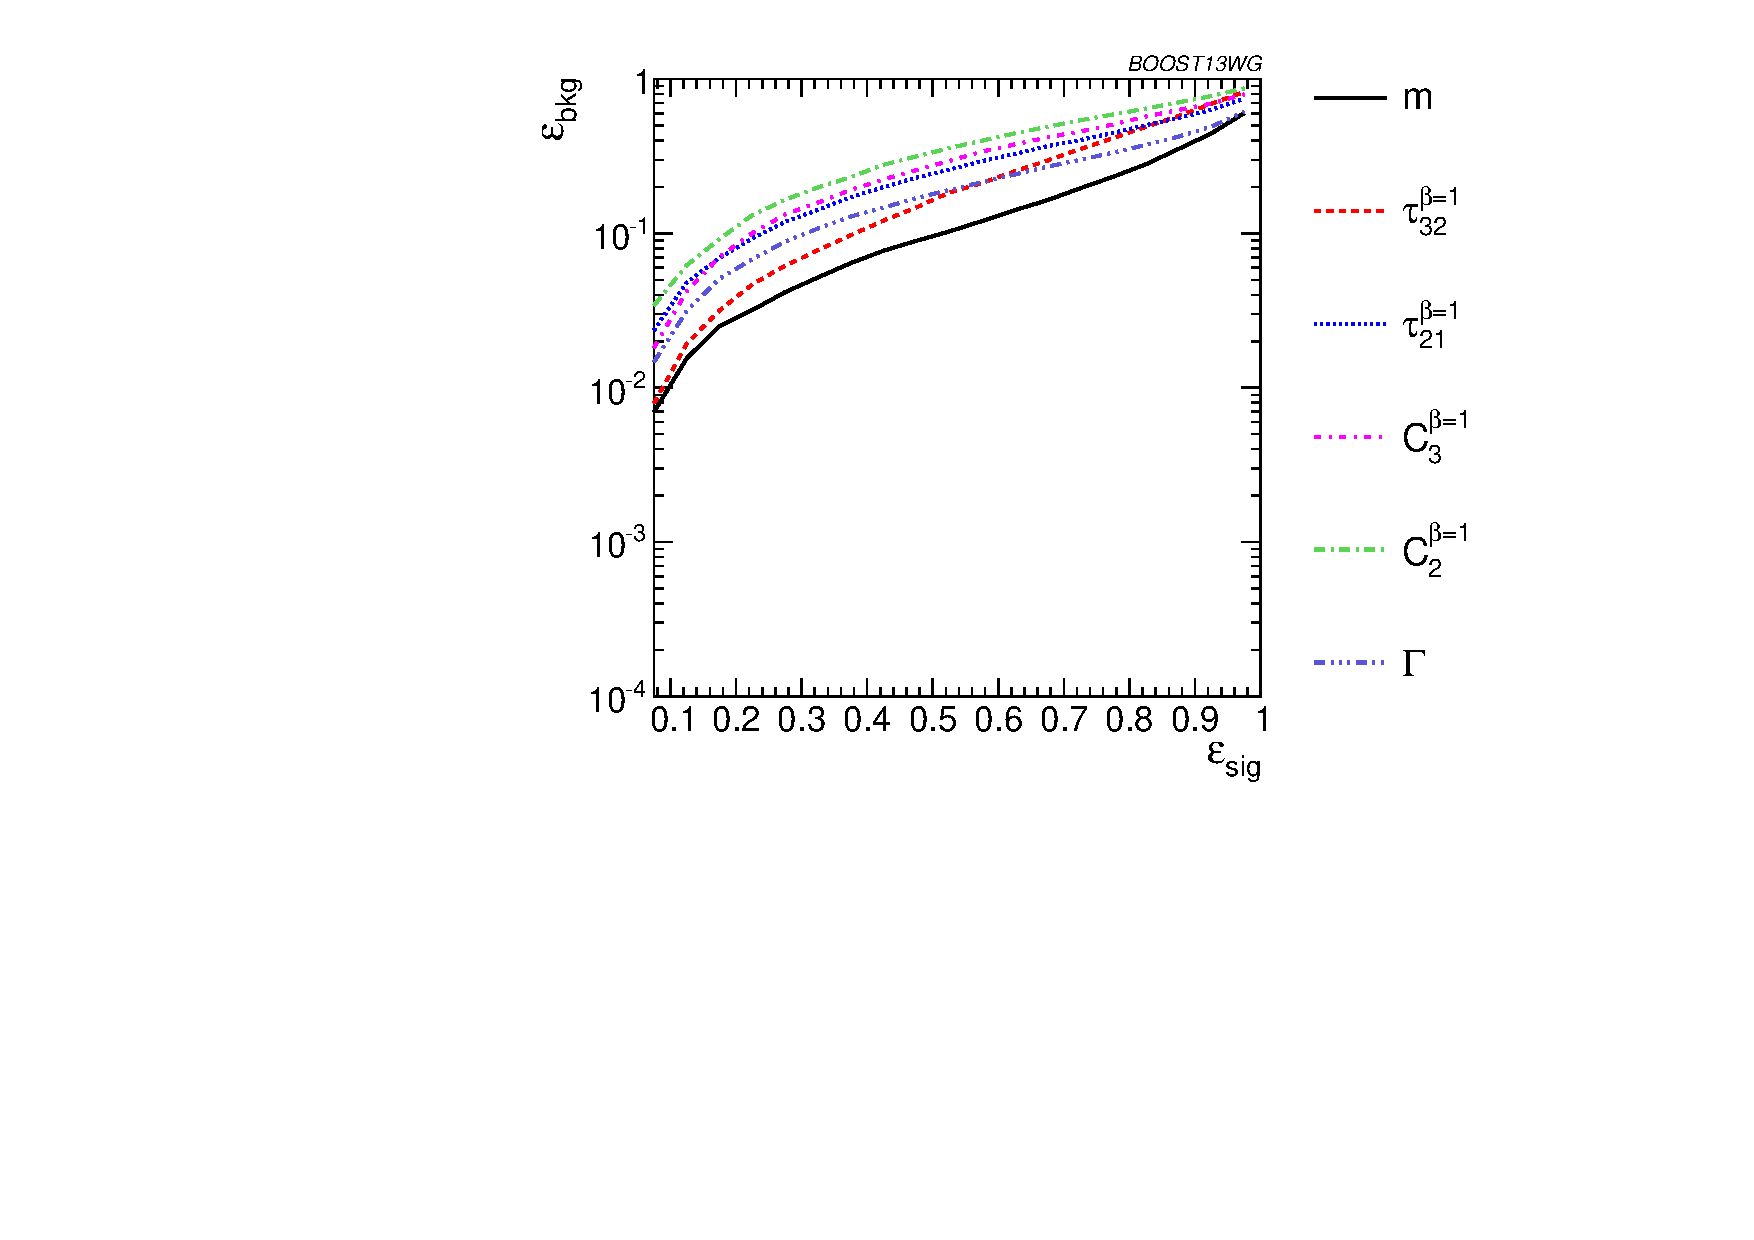
\includegraphics[width=0.49\textwidth]{./Figures/TTagging/single_variable/pT.1TeV.R.0.8/Rocs_shape.pdf}\label{fig:single_variable_ROC_shape}}
\subfigure[Top mass]{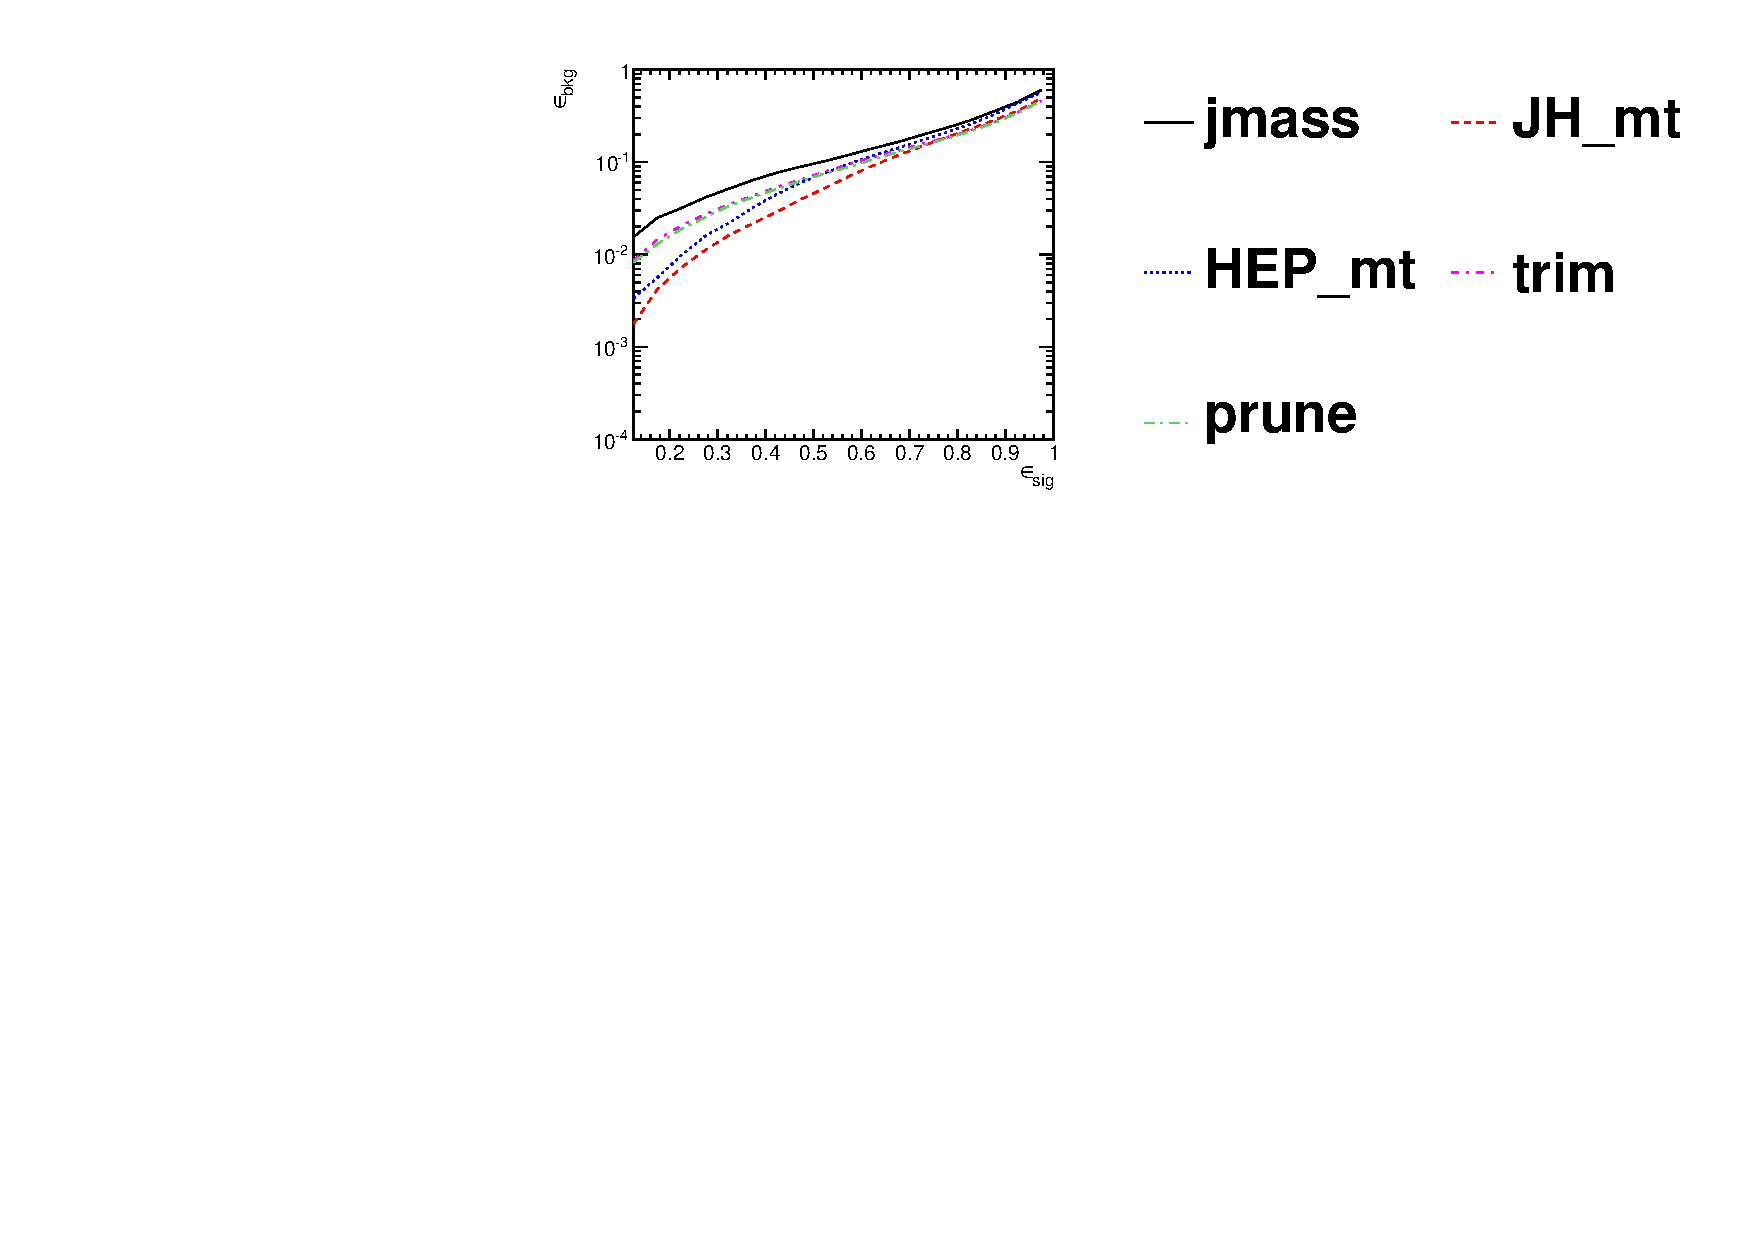
\includegraphics[width=0.49\textwidth]{./Figures/TTagging/single_variable/pT.1TeV.R.0.8/Rocs_top_mass.pdf}}
\subfigure[$W$ mass]{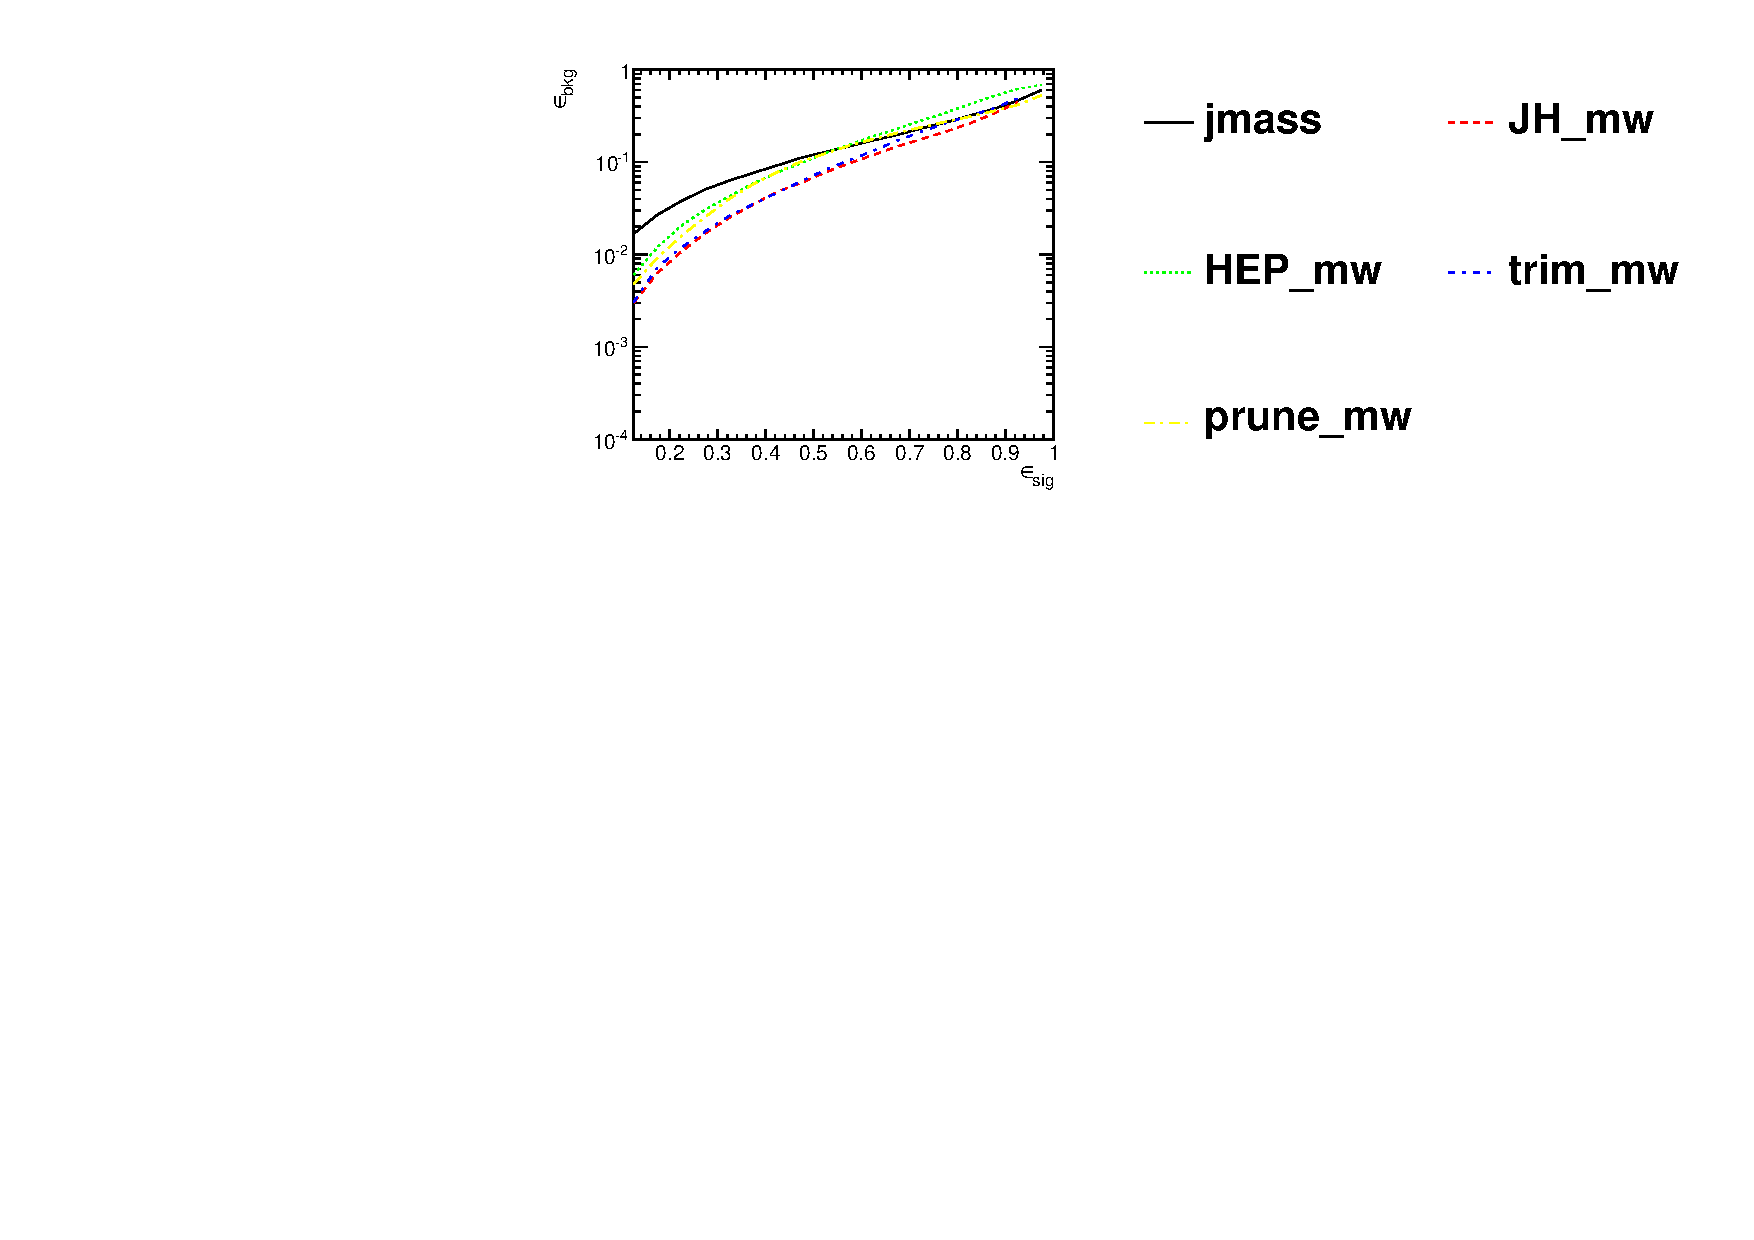
\includegraphics[width=0.49\textwidth]{./Figures/TTagging/single_variable/pT.1TeV.R.0.8/Rocs_w_mass.pdf}}
\caption{Comparison of single-variable top-tagging performance in the $\pt= 1-1.1$ GeV bin using the anti-\kT, R=0.8 algorithm.}
\label{fig:single_variable_ROC}
\end{figure*}

Of the two top tagging algorithms, we can see from Figure~\ref{fig:single_variable_ROC} that the Johns Hopkins (JH) tagger out-performs the HEPTopTagger in terms of its signal-to-background separation power in both the top and $W$ candidate masses; this is expected, as the HEPTopTagger was designed to reconstruct moderate \pt top jets in $ttH$ events (for a proposal for a high-\pt variant of the HEPTopTagger, see \cite{Schaetzel:2013vka}). In Figure~\ref{fig:topmass_histogram_HEP_JH} we show the histograms for the top mass output from the JH and HEPTopTagger for different $R$ in the \pt 1.5-1.6 TeV bin, and in Figure~\ref{fig:topmass_histogram_HEP_JH_pT} for different \pt at at R =0.8, optimized at a signal efficiency of 30\%. One can see from these figures that the likely reason for the better performance of the JH tagger is that, in the HEPTopTagger algorithm, the jet is filtered to select the five hardest subjets, and then three subjets are chosen which reconstruct the top mass. This requirement tends to shape a peak in the QCD background around $m_t$ for the HEPTopTagger, while the JH tagger has no such requirement. It has been suggested  \cite{Anders:2013oga} that performance in the HEPTopTagger may be improved by selecting the three subjets reconstructing the top only among those that pass the $W$ mass constraints, which somewhat reduces the shaping of the background. The discrepancy between the JH and HEPTopTaggers is more pronounced  at higher $\pt$ and larger jet radius (see Figs.~\ref{fig:ptcomparison_singletopmass_top} and \ref{fig:Rcomparison_singletopmass_top}). 

\begin{figure*}
\centering
\subfigure[JH, $R=0.4$]{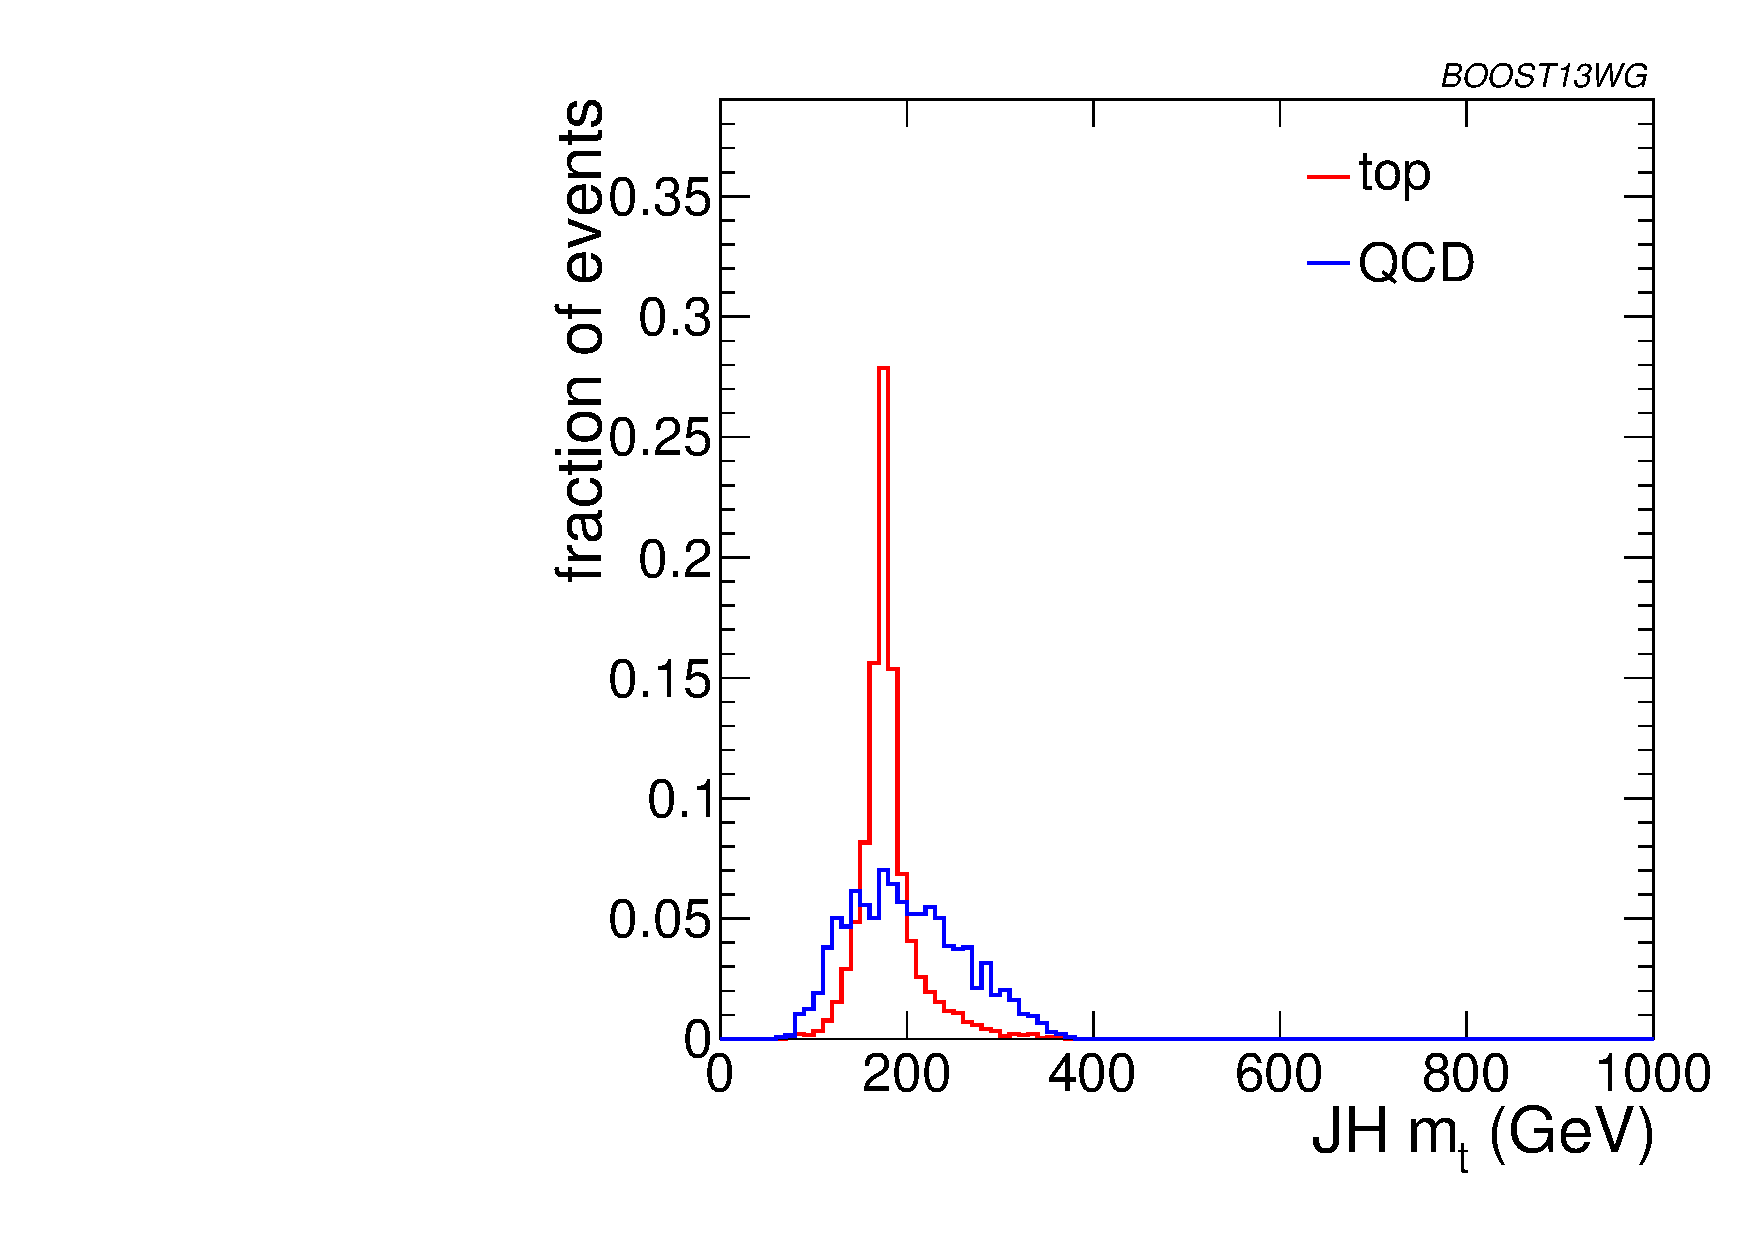
\includegraphics[width=0.245\textwidth]{./Figures/TTagging/single_variable/pT.1.5TeV.R.0.4/h_JH_mt_opt_mt.pdf}}
\subfigure[HEP, $R=0.4$]{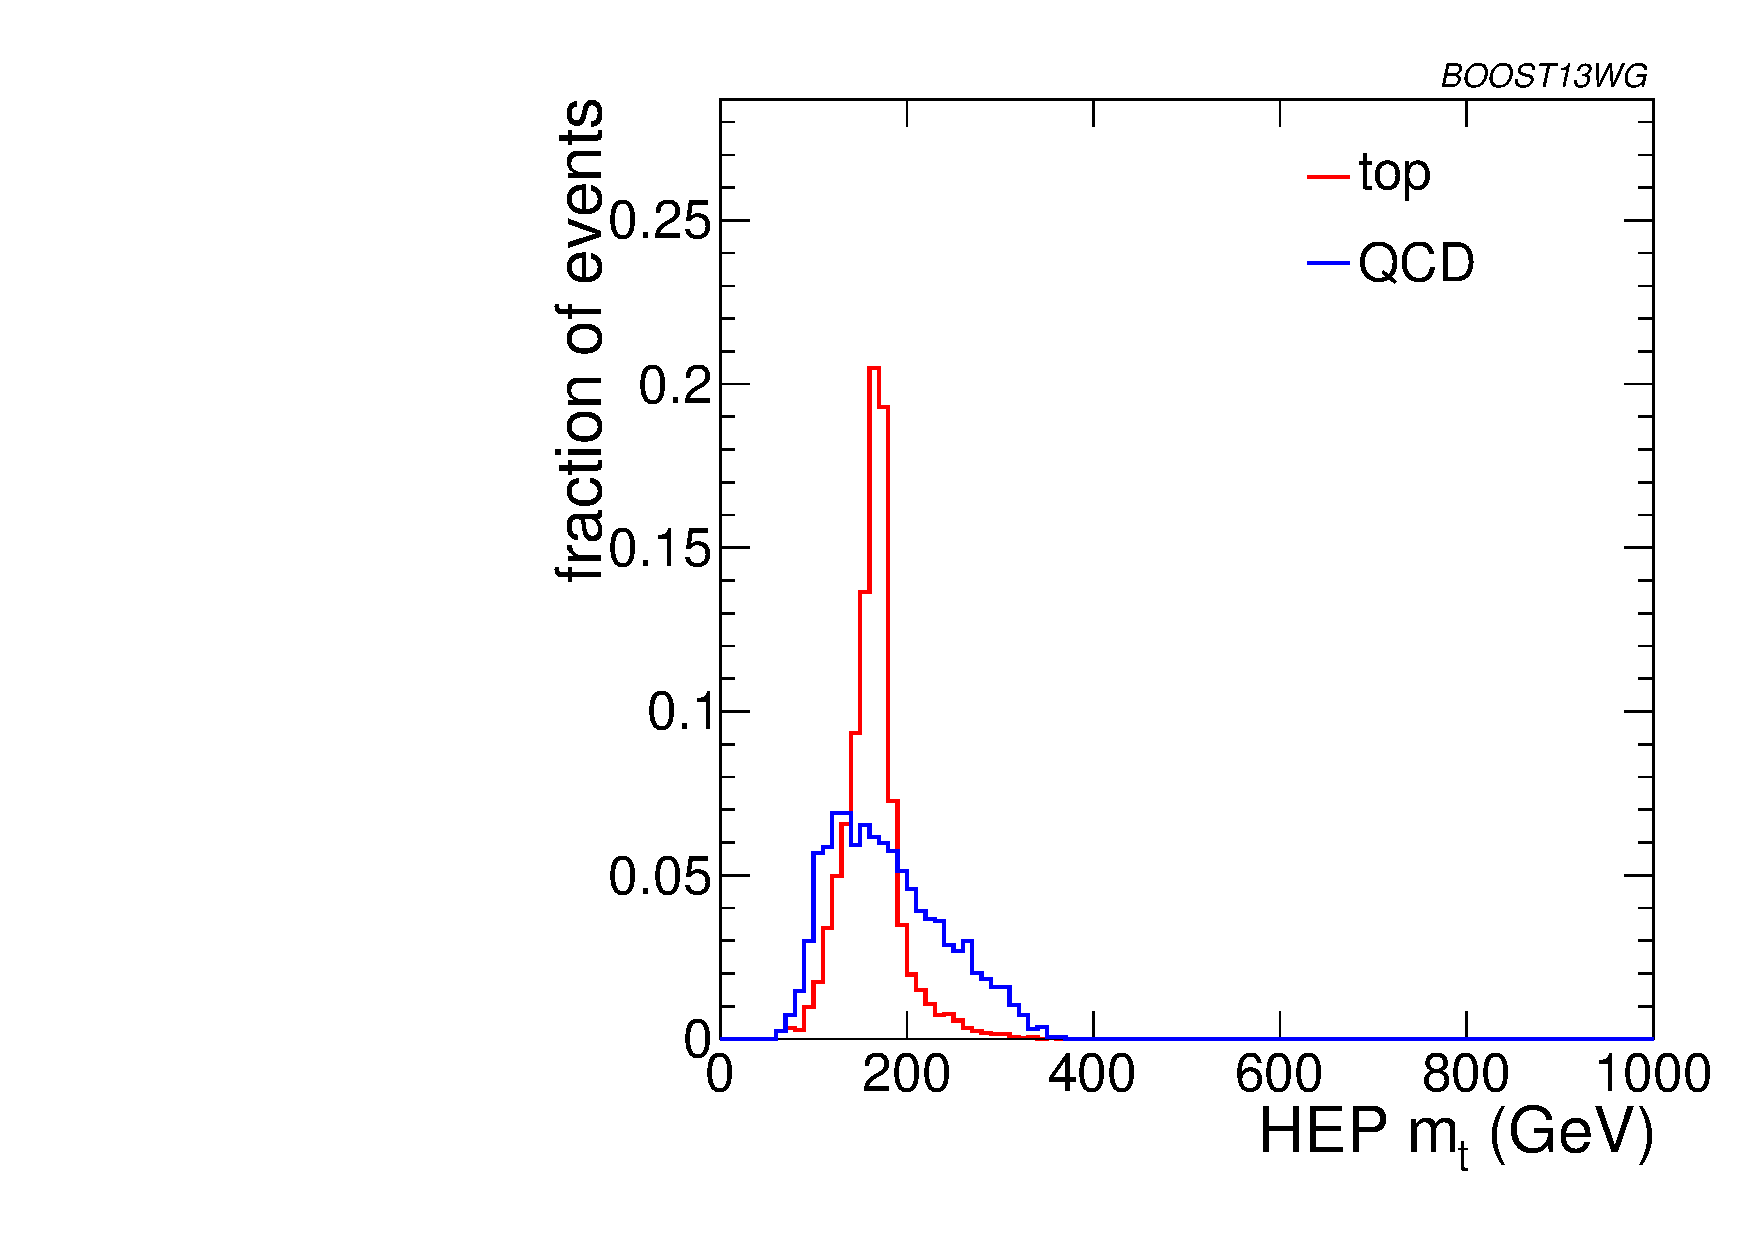
\includegraphics[width=0.245\textwidth]{./Figures/TTagging/single_variable/pT.1.5TeV.R.0.4/h_HEP_mt_opt_mt.pdf}}
\subfigure[JH, $R=1.2$]{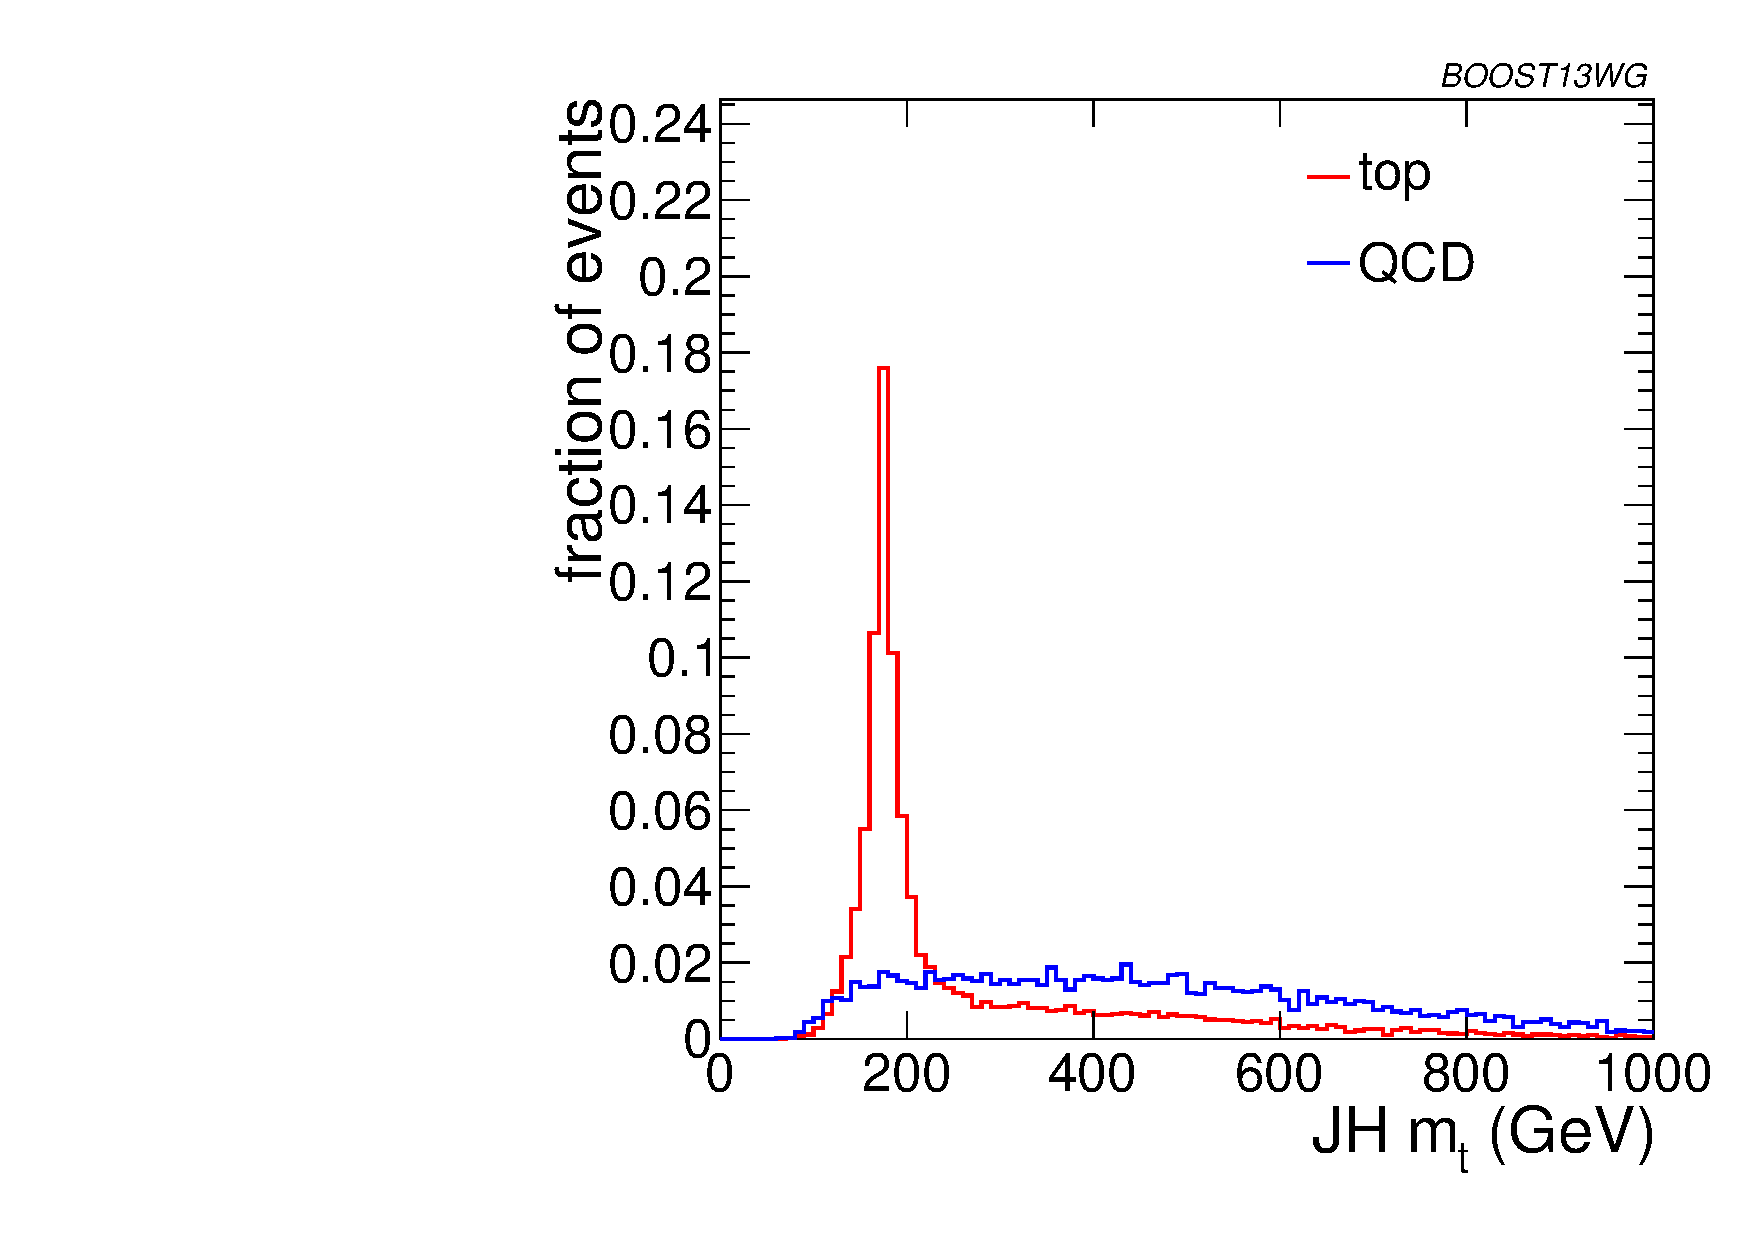
\includegraphics[width=0.245\textwidth]{./Figures/TTagging/single_variable/pT.1.5TeV.R.1.2/h_JH_mt_opt_mt.pdf}}
\subfigure[HEP, $R=1.2$]{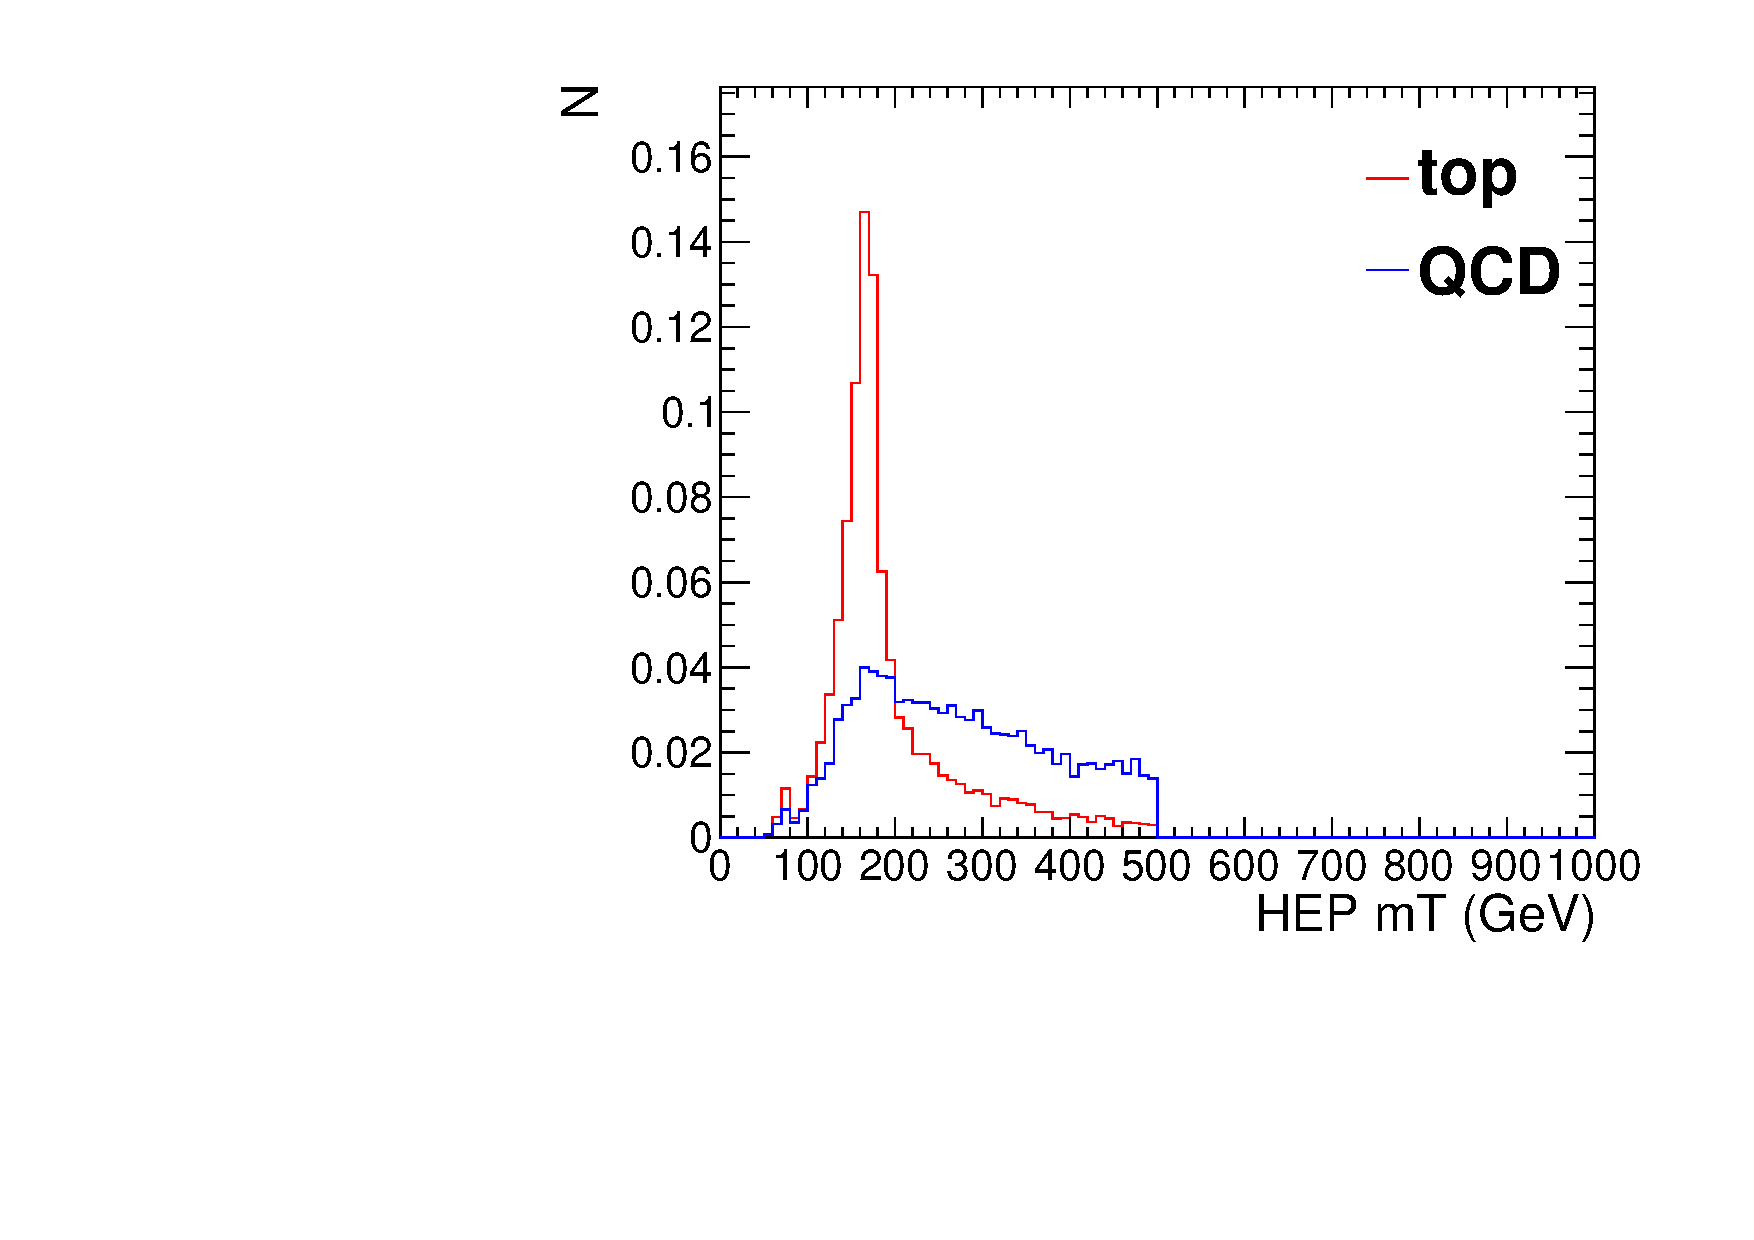
\includegraphics[width=0.245\textwidth]{./Figures/TTagging/single_variable/pT.1.5TeV.R.1.2/h_HEP_mt_opt_mt.pdf}}\\
\subfigure[prune, $R=0.4$]{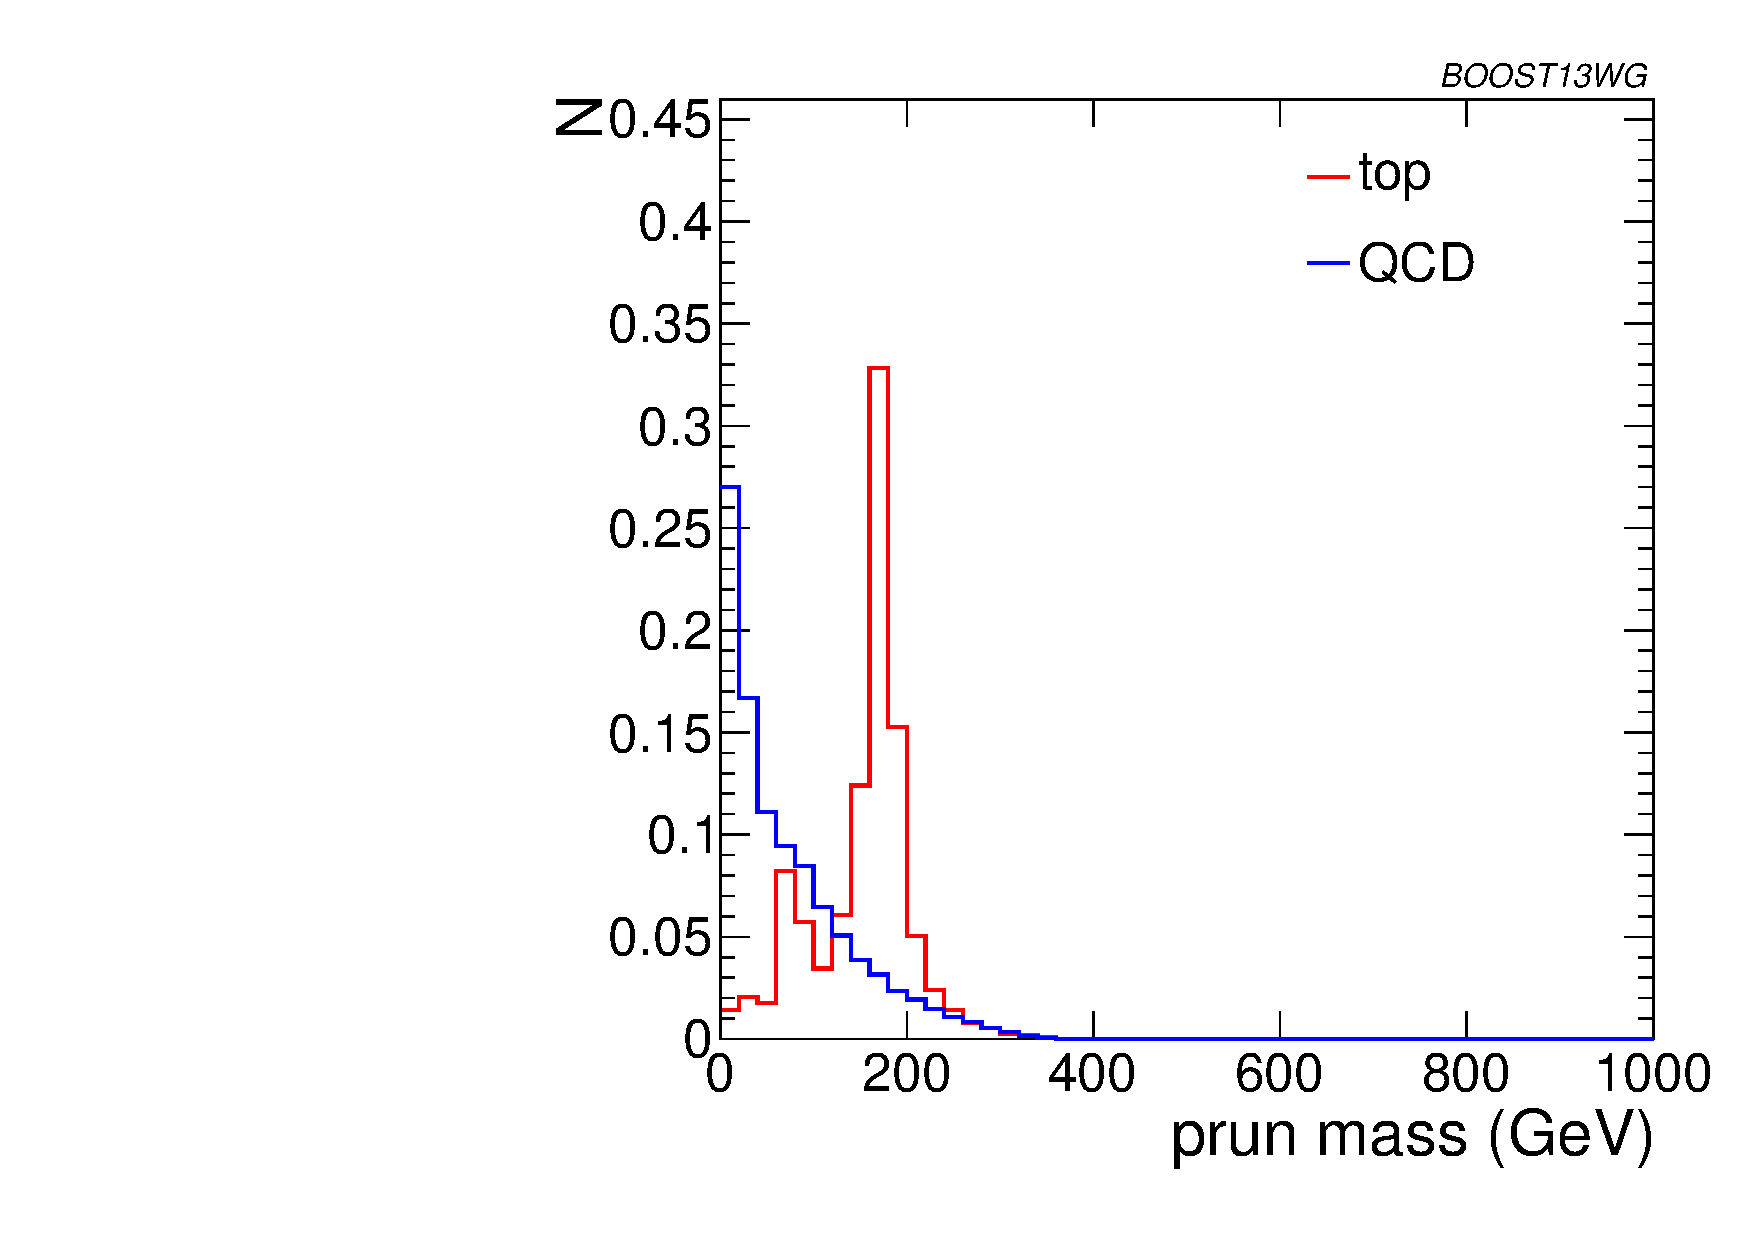
\includegraphics[width=0.245\textwidth]{./Figures/TTagging/single_variable/pT.1.5TeV.R.0.4/h_prun_R_0_4.pdf}}
\subfigure[trim, $R=0.4$]{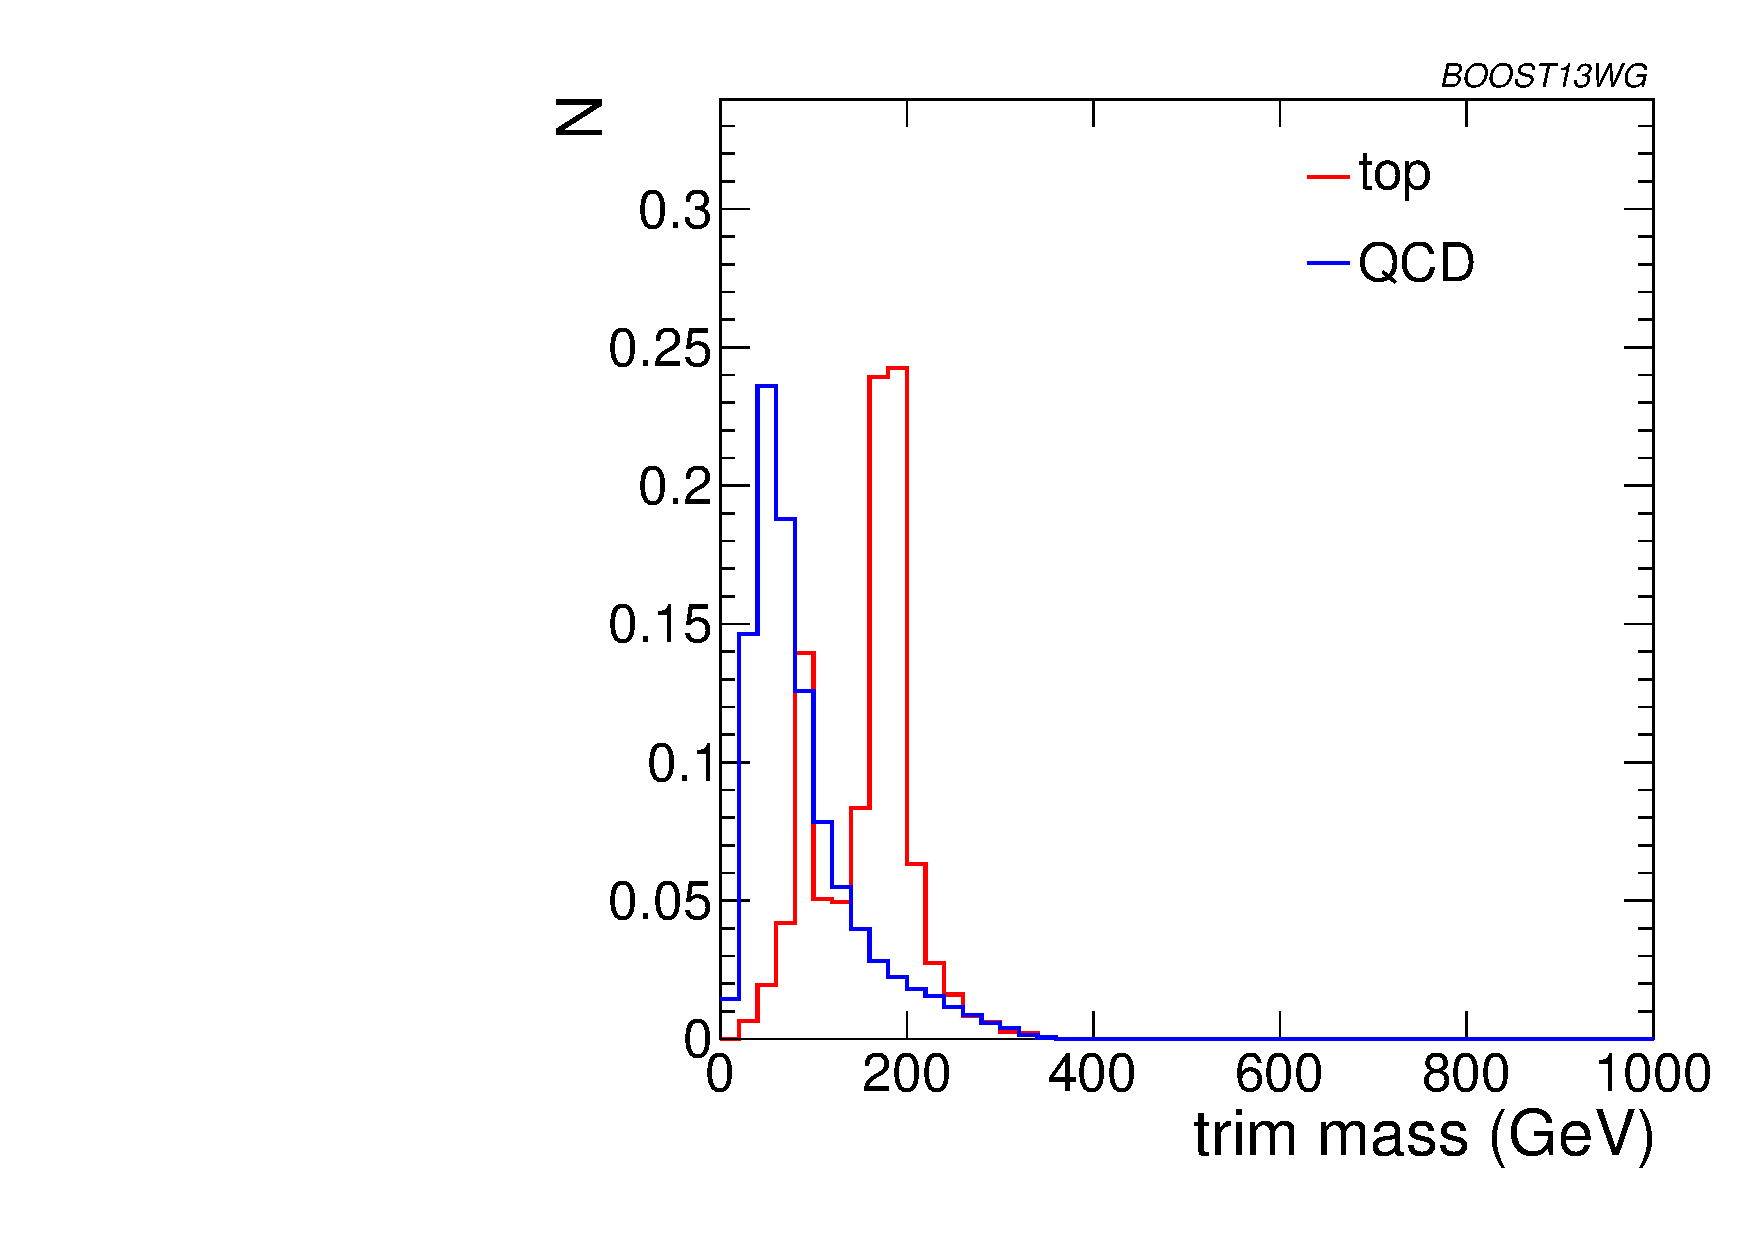
\includegraphics[width=0.245\textwidth]{./Figures/TTagging/single_variable/pT.1.5TeV.R.0.4/h_trim_R_0_4.pdf}}
\subfigure[prune, $R=1.2$]{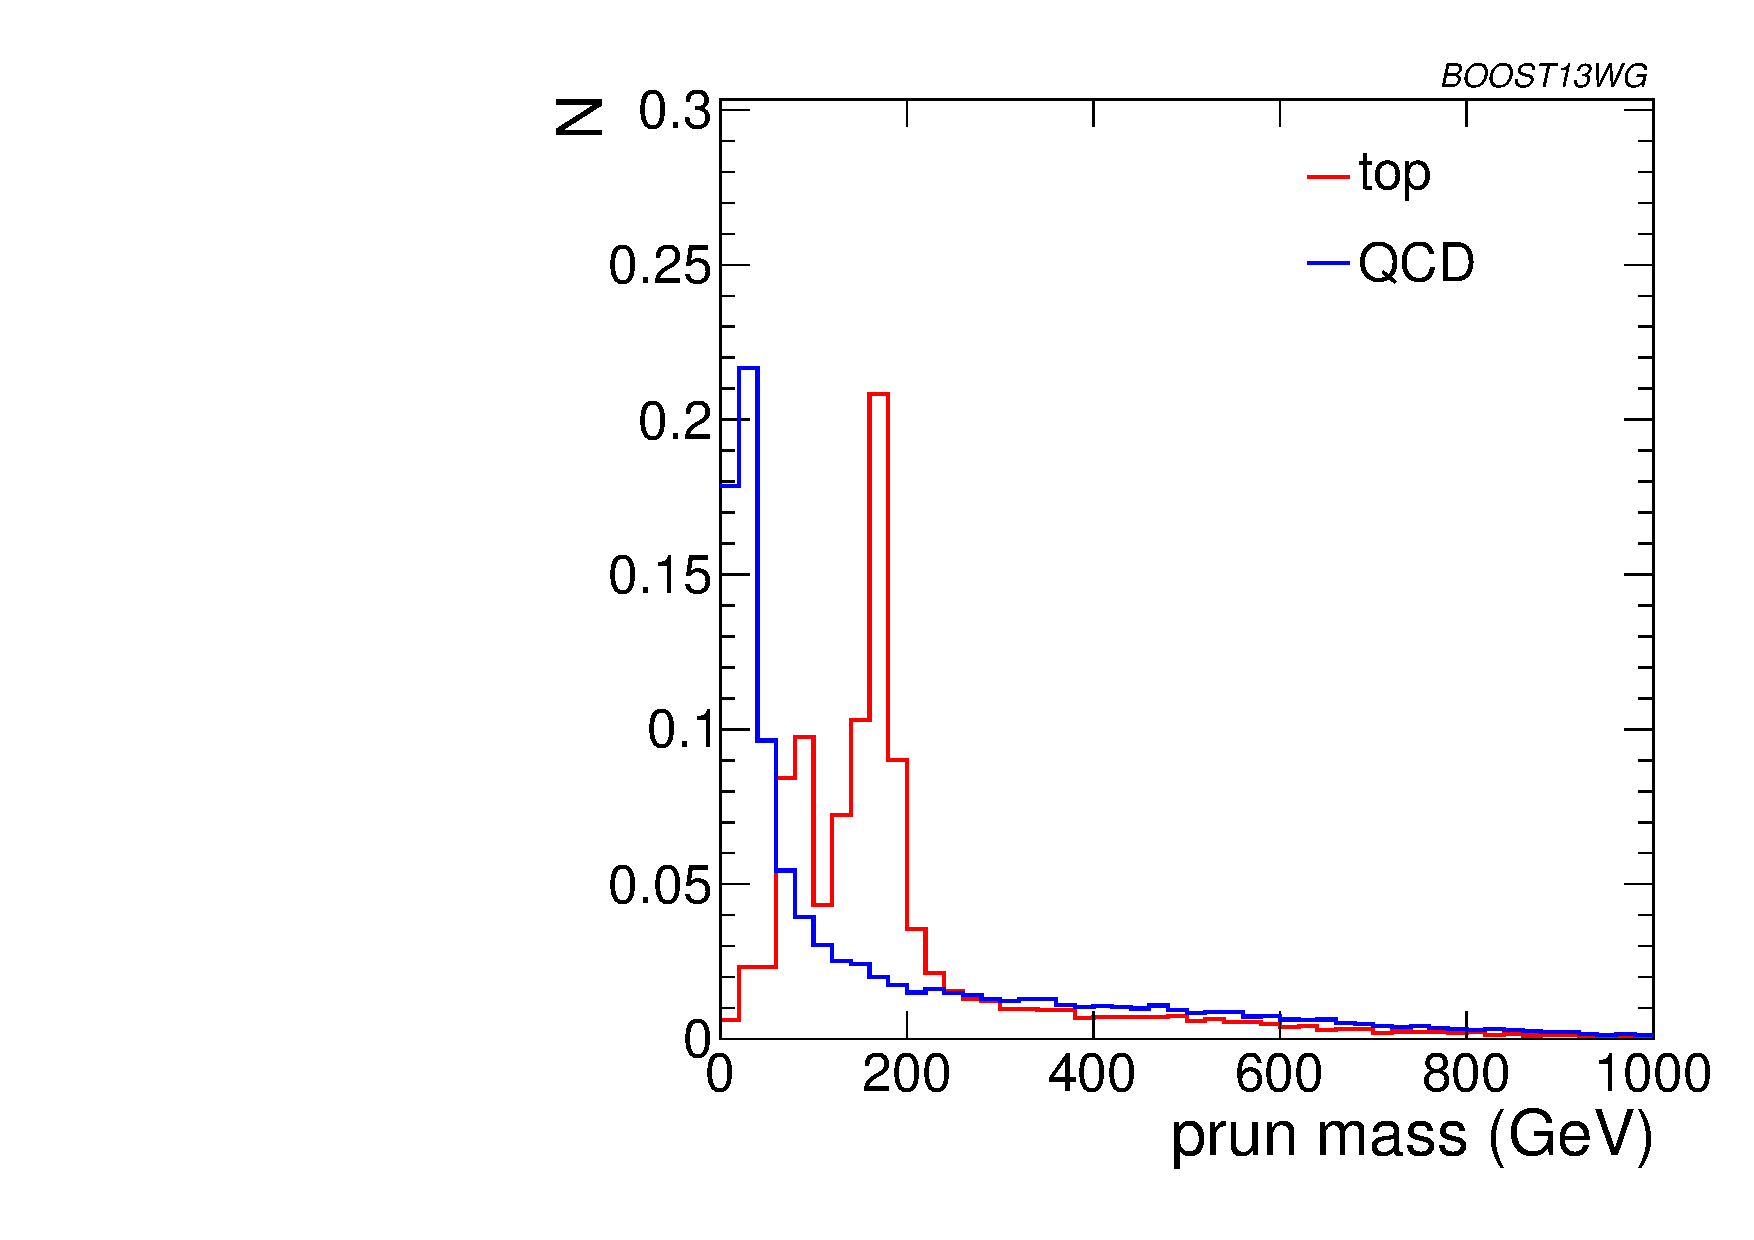
\includegraphics[width=0.245\textwidth]{./Figures/TTagging/single_variable/pT.1.5TeV.R.1.2/h_prun_R_1_2.pdf}}
\subfigure[trim, $R=1.2$]{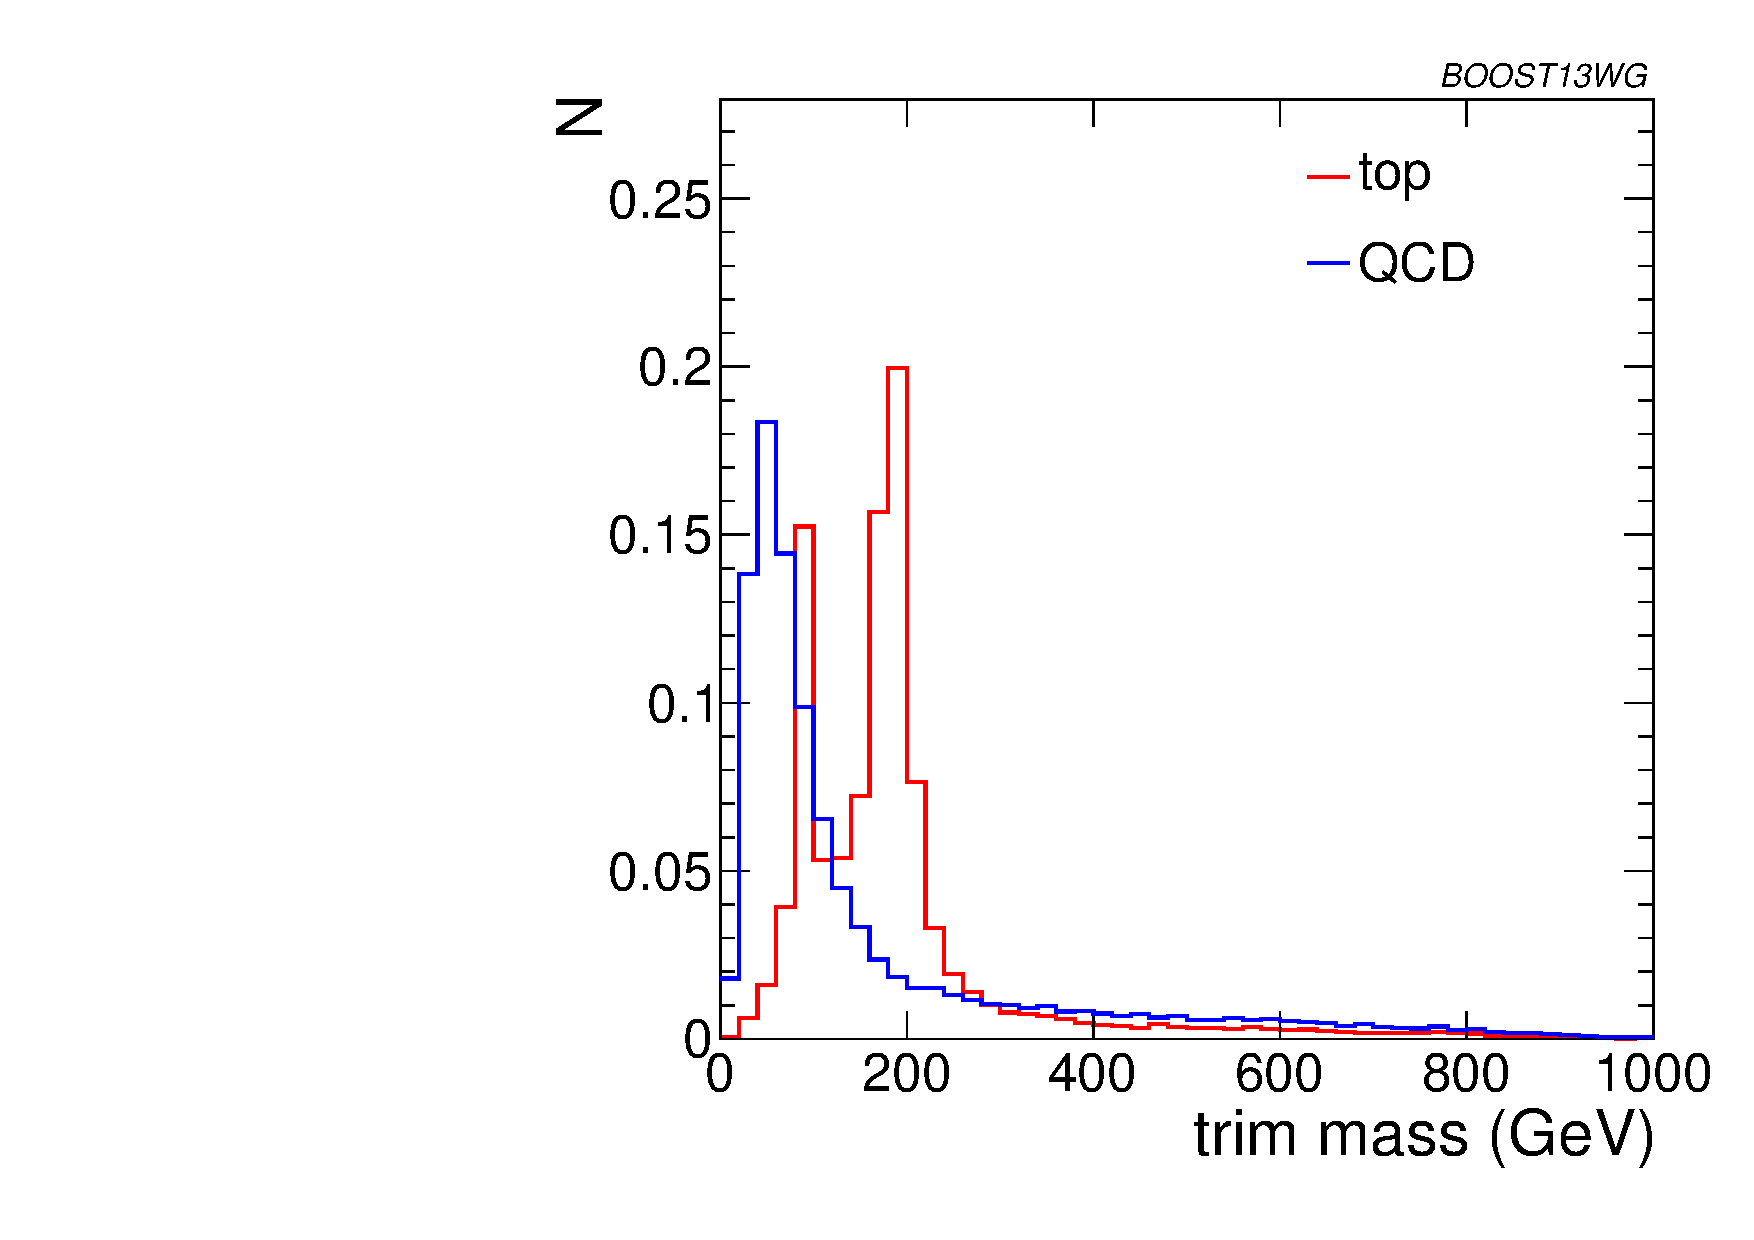
\includegraphics[width=0.245\textwidth]{./Figures/TTagging/single_variable/pT.1.5TeV.R.1.2/h_trim_R_1_2.pdf}}
\caption{Comparison of top mass reconstruction with the Johns Hopkins (JH), HEPTopTaggers (HEP), pruning, and trimming at different $R$ using the anti-\kT algorithm, $p_{\rm T}=1.5-1.6$ TeV. Each histogram is shown for the working point optimized for best performance with $m_t$ in the $0.3-0.35$ signal efficiency bin, and is normalized to the fraction of events passing the tagger. In this and subsequent plots, the HEPTopTagger distribution cuts off at 500 GeV because the tagger fails to tag jets with a larger mass.}
\label{fig:topmass_histogram_HEP_JH}
\end{figure*}

\begin{figure*}
\centering
\subfigure[JH, $\pt=600-700$ GeV]{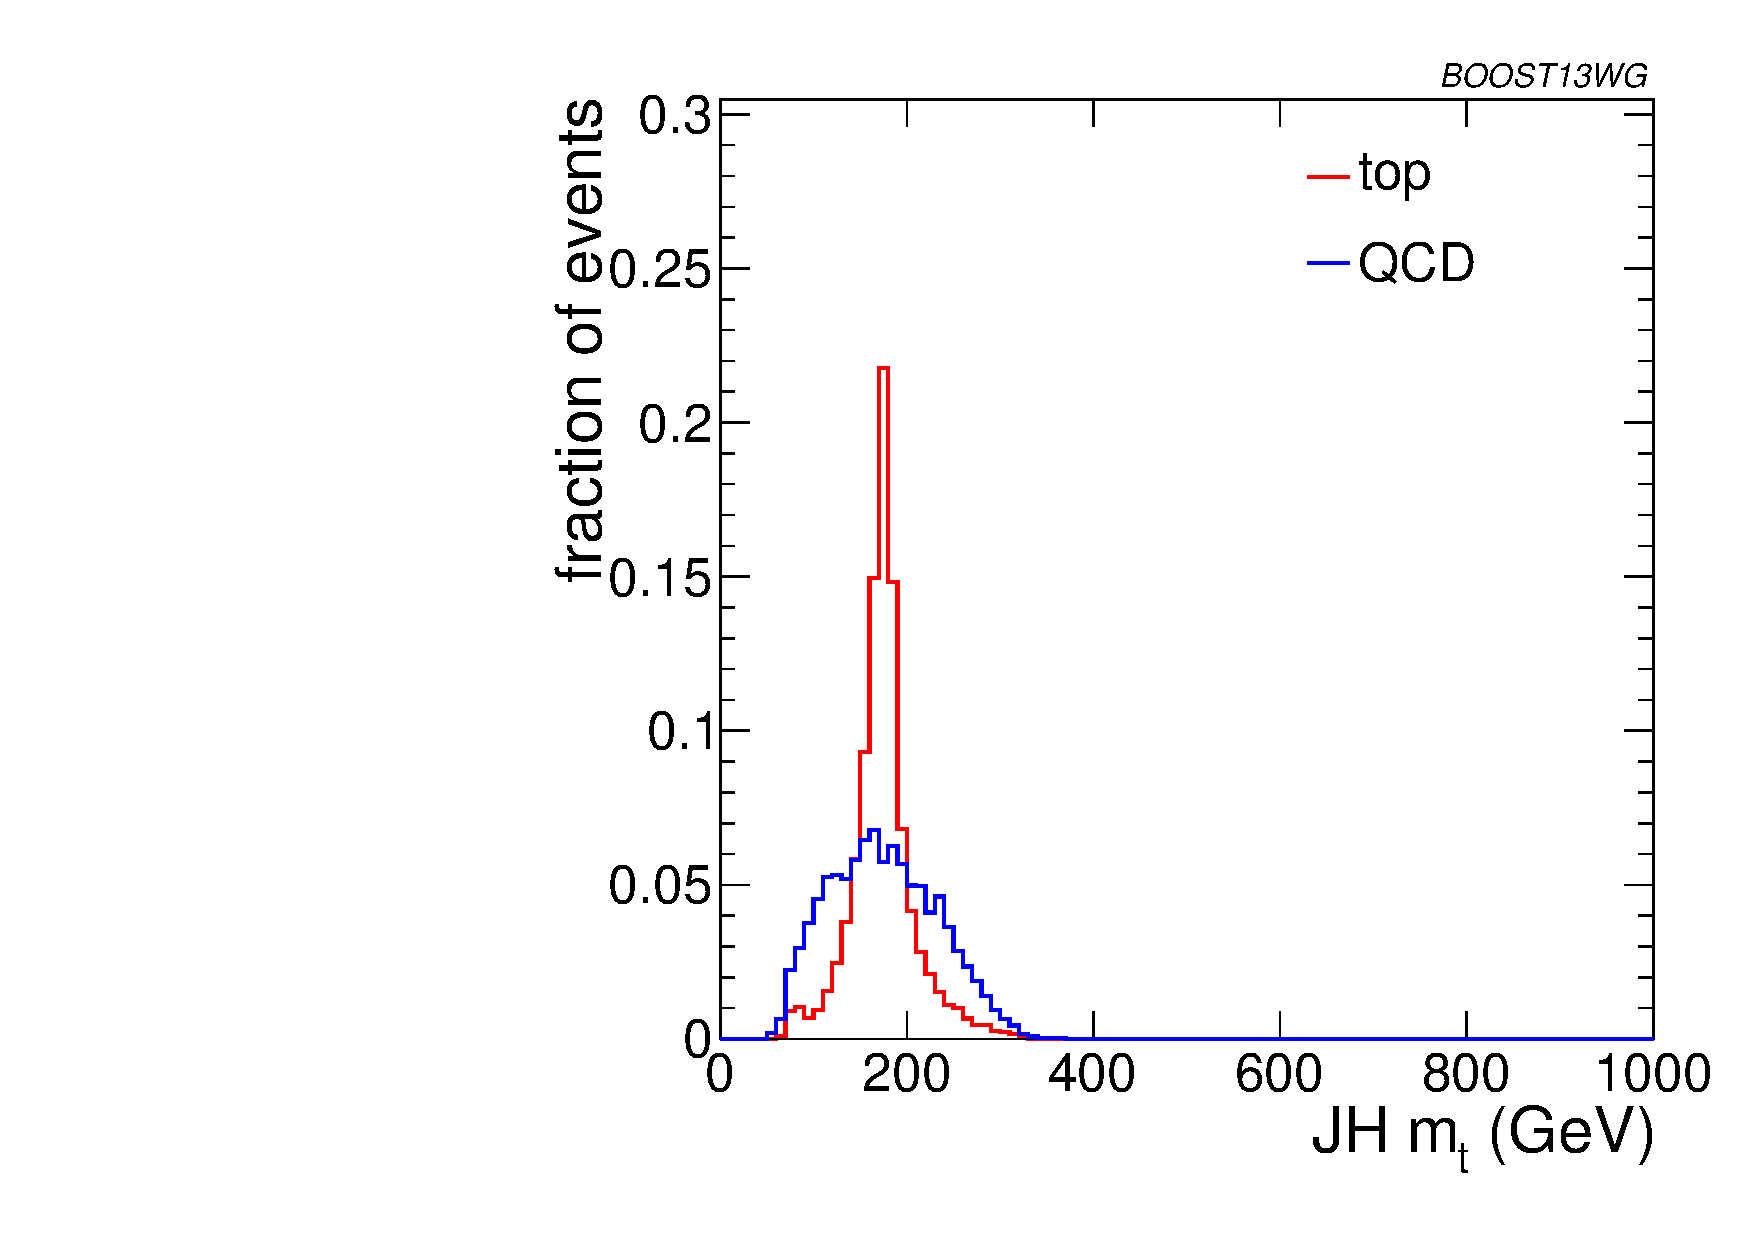
\includegraphics[width=0.245\textwidth]{./Figures/TTagging/single_variable/pT.600GeV.R.0.8/h_JH_mt_pT_0_6.pdf}}
\subfigure[HEP, $\pt=600-700$ GeV]{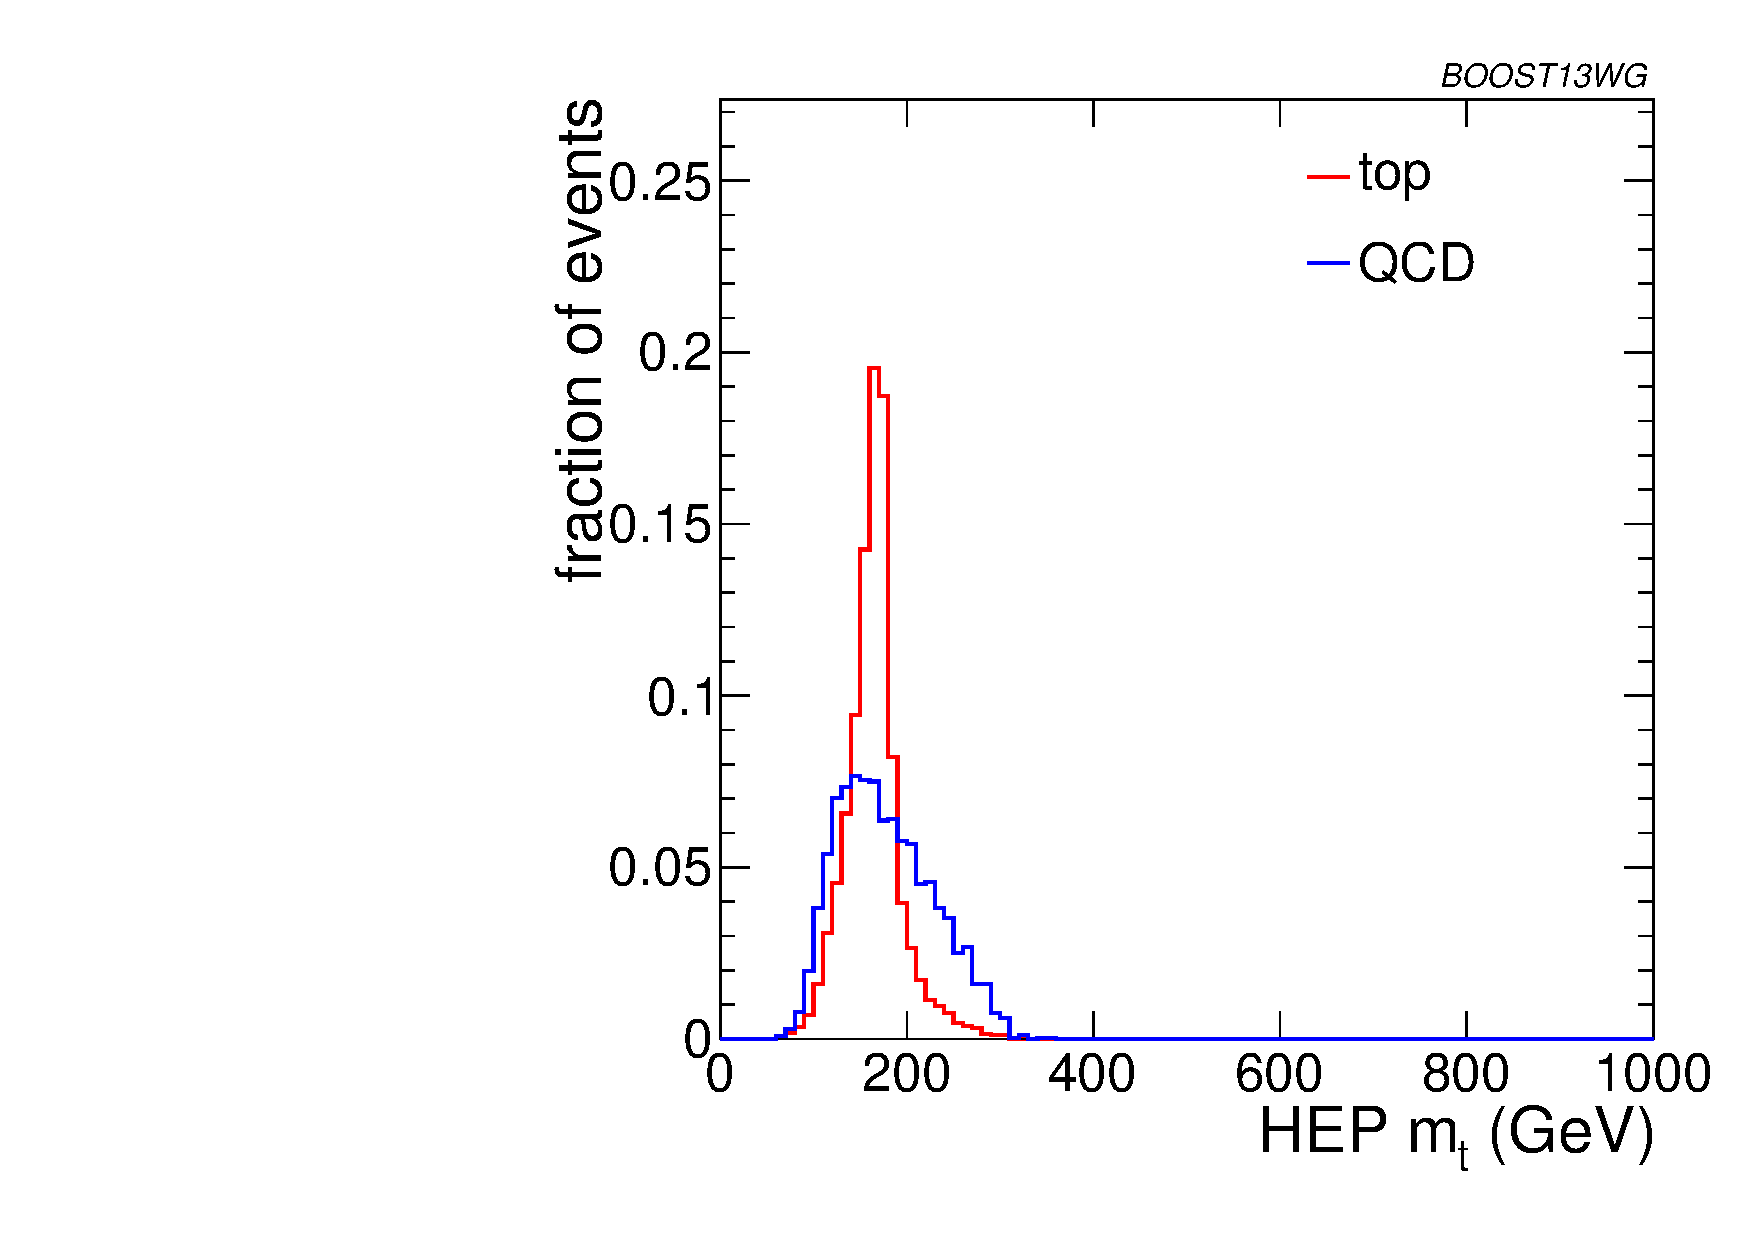
\includegraphics[width=0.245\textwidth]{./Figures/TTagging/single_variable/pT.600GeV.R.0.8/h_HEP_mt_pT_0_6.pdf}}
\subfigure[JH, $\pt=1.5-1.6$ TeV]{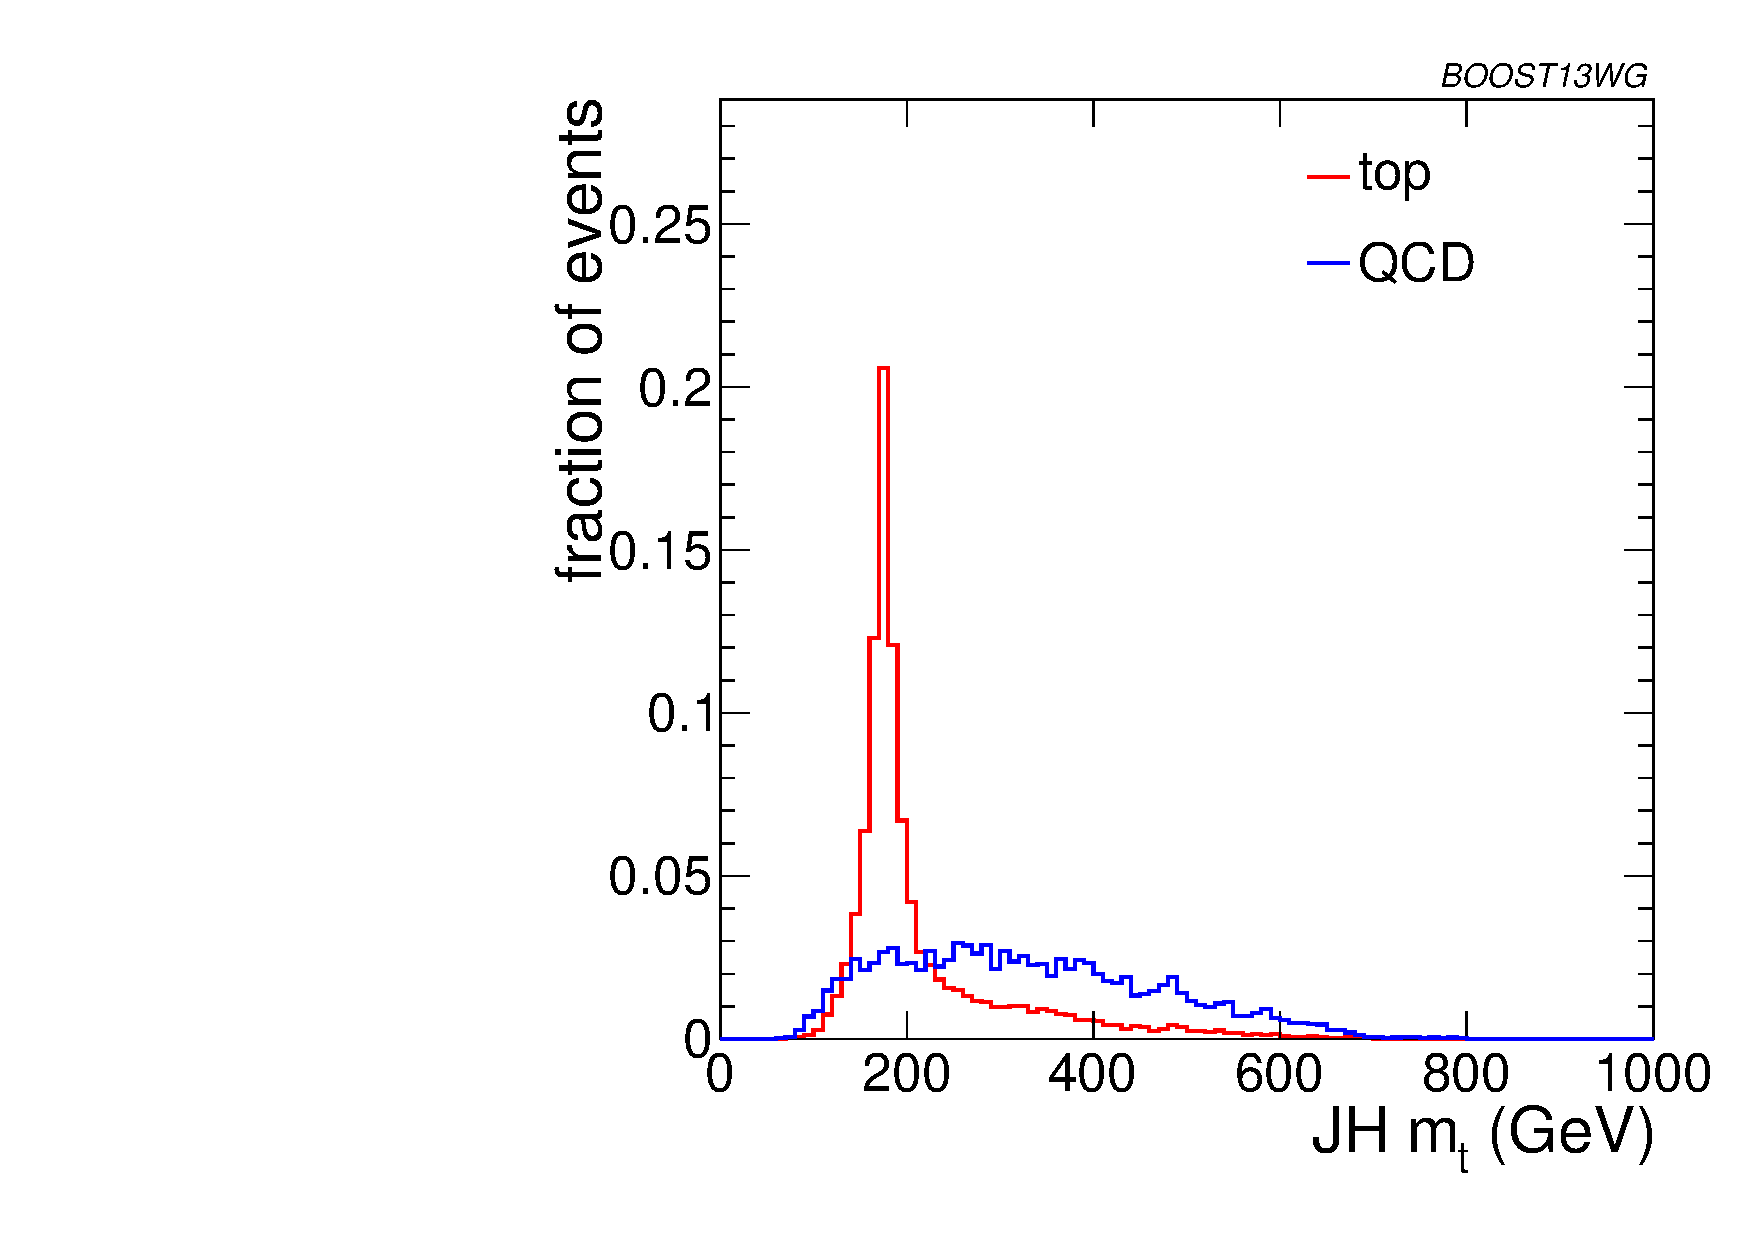
\includegraphics[width=0.245\textwidth]{./Figures/TTagging/single_variable/pT.1.5TeV.R.0.8/h_JH_mt_pT_1_5.pdf}}
\subfigure[HEP, $\pt=1.5-1.6$ TeV]{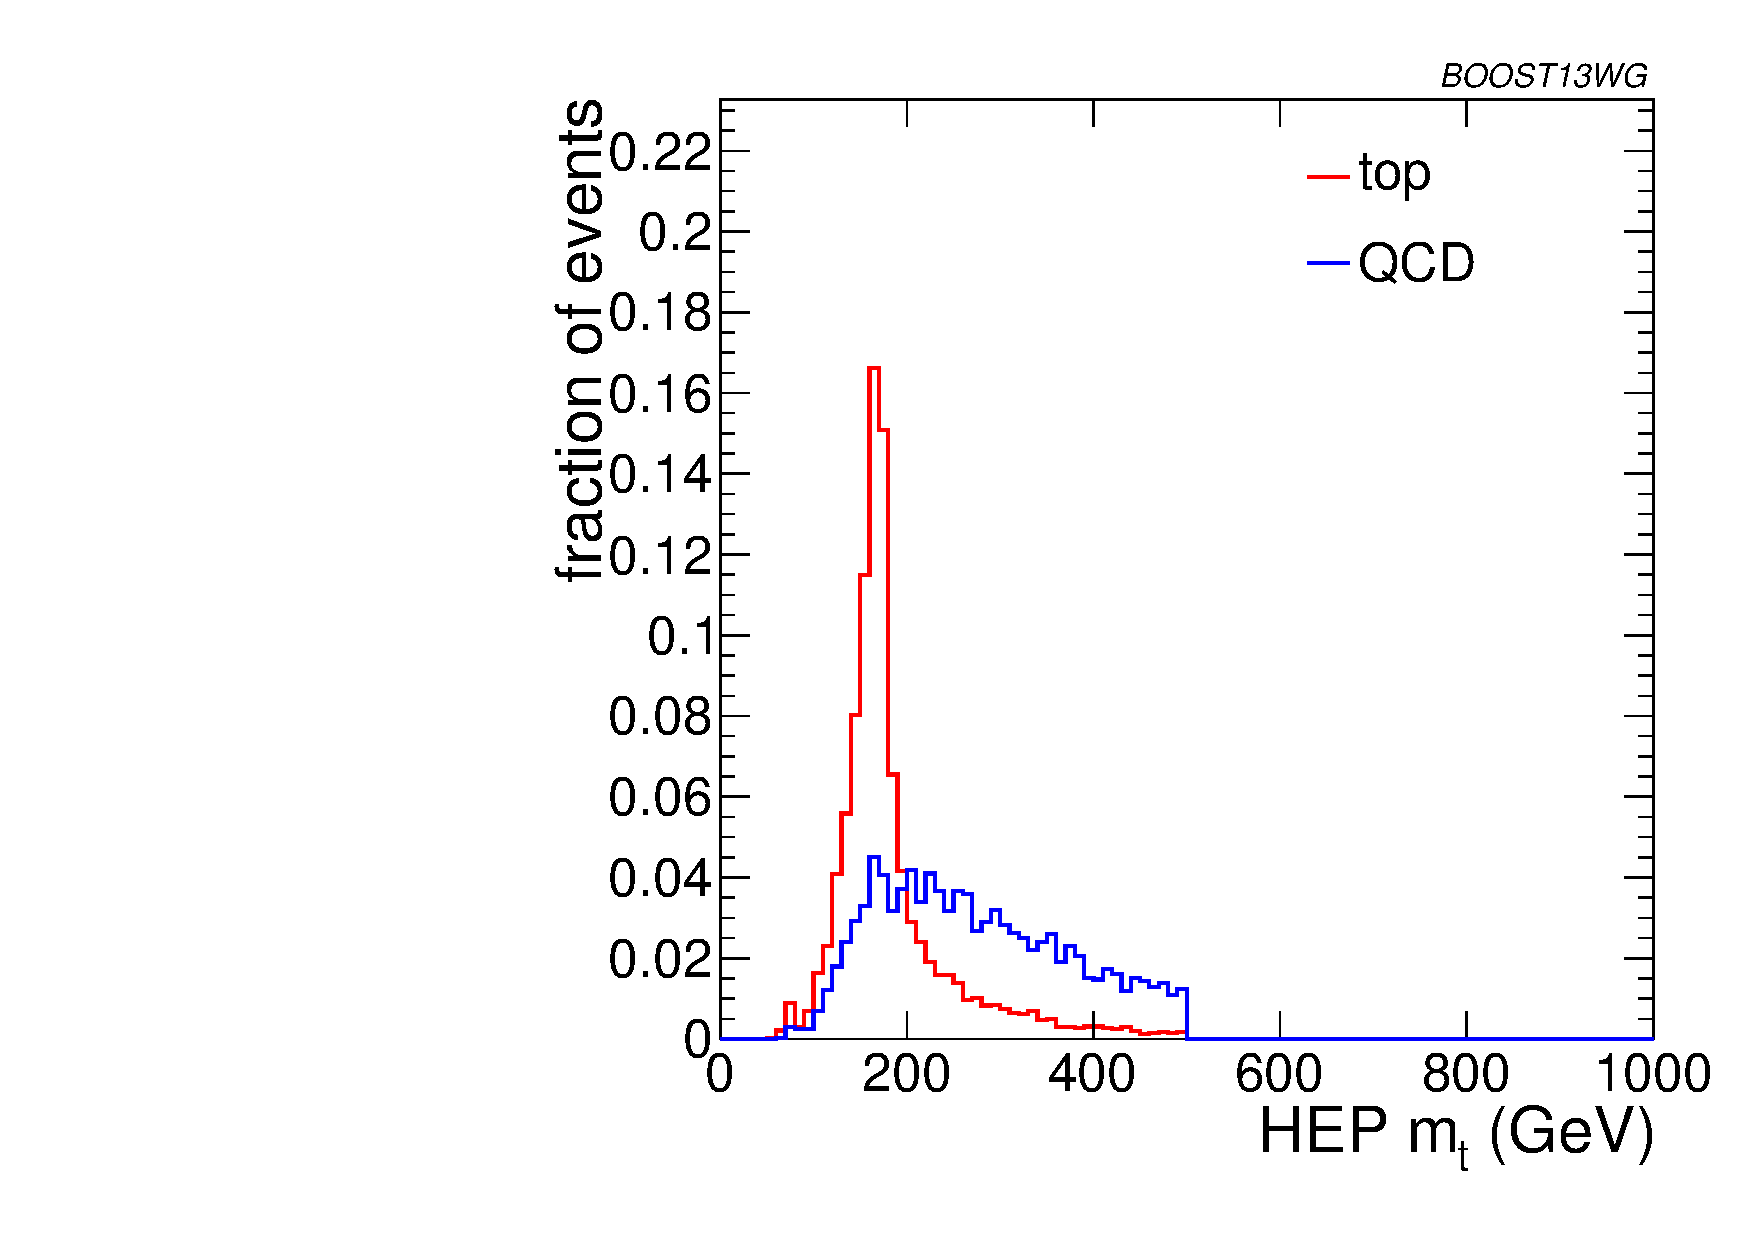
\includegraphics[width=0.245\textwidth]{./Figures/TTagging/single_variable/pT.1.5TeV.R.0.8/h_HEP_mt_pT_1_5.pdf}}\\
\subfigure[prune, $\pt=600-700$ GeV]{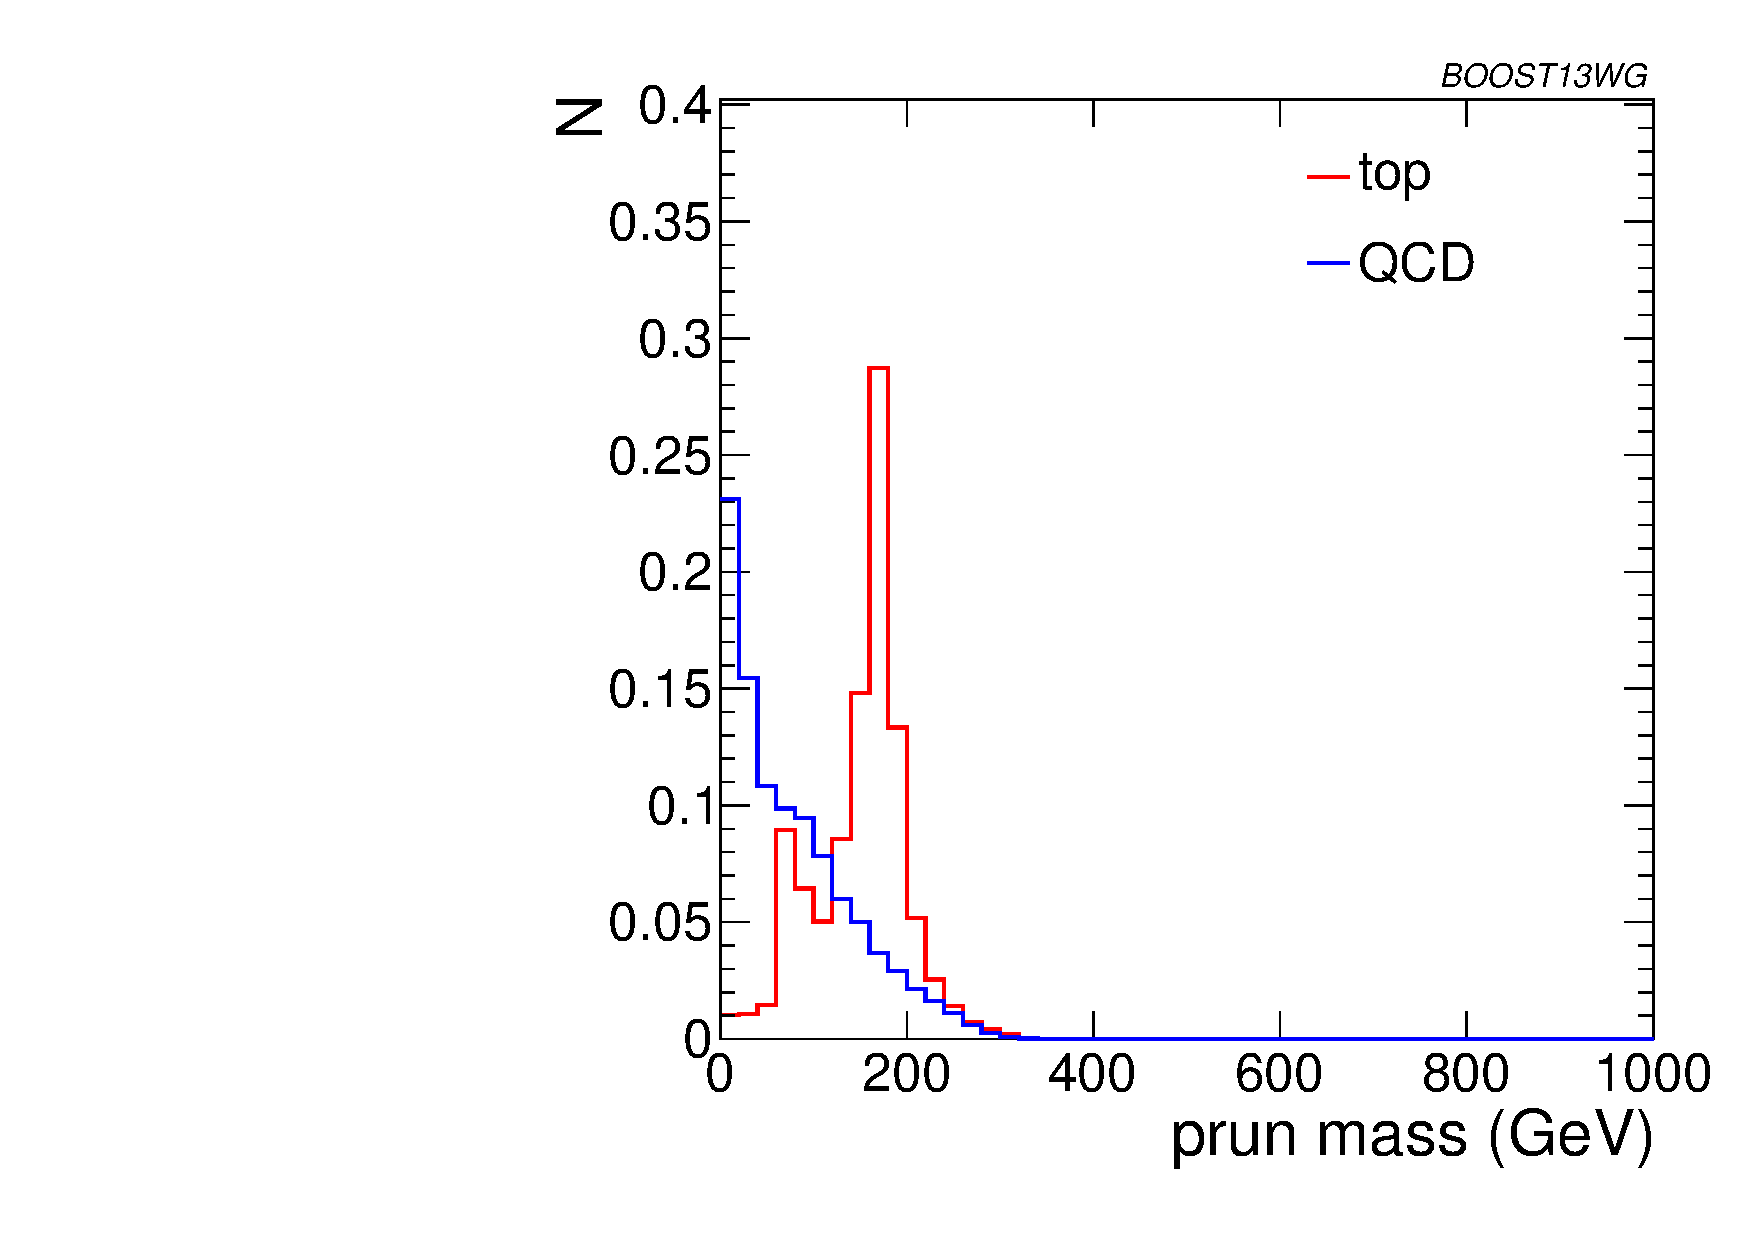
\includegraphics[width=0.245\textwidth]{./Figures/TTagging/single_variable/pT.600GeV.R.0.8/h_prun_pT_0_6.pdf}}
\subfigure[trim, $\pt=600-700$ GeV]{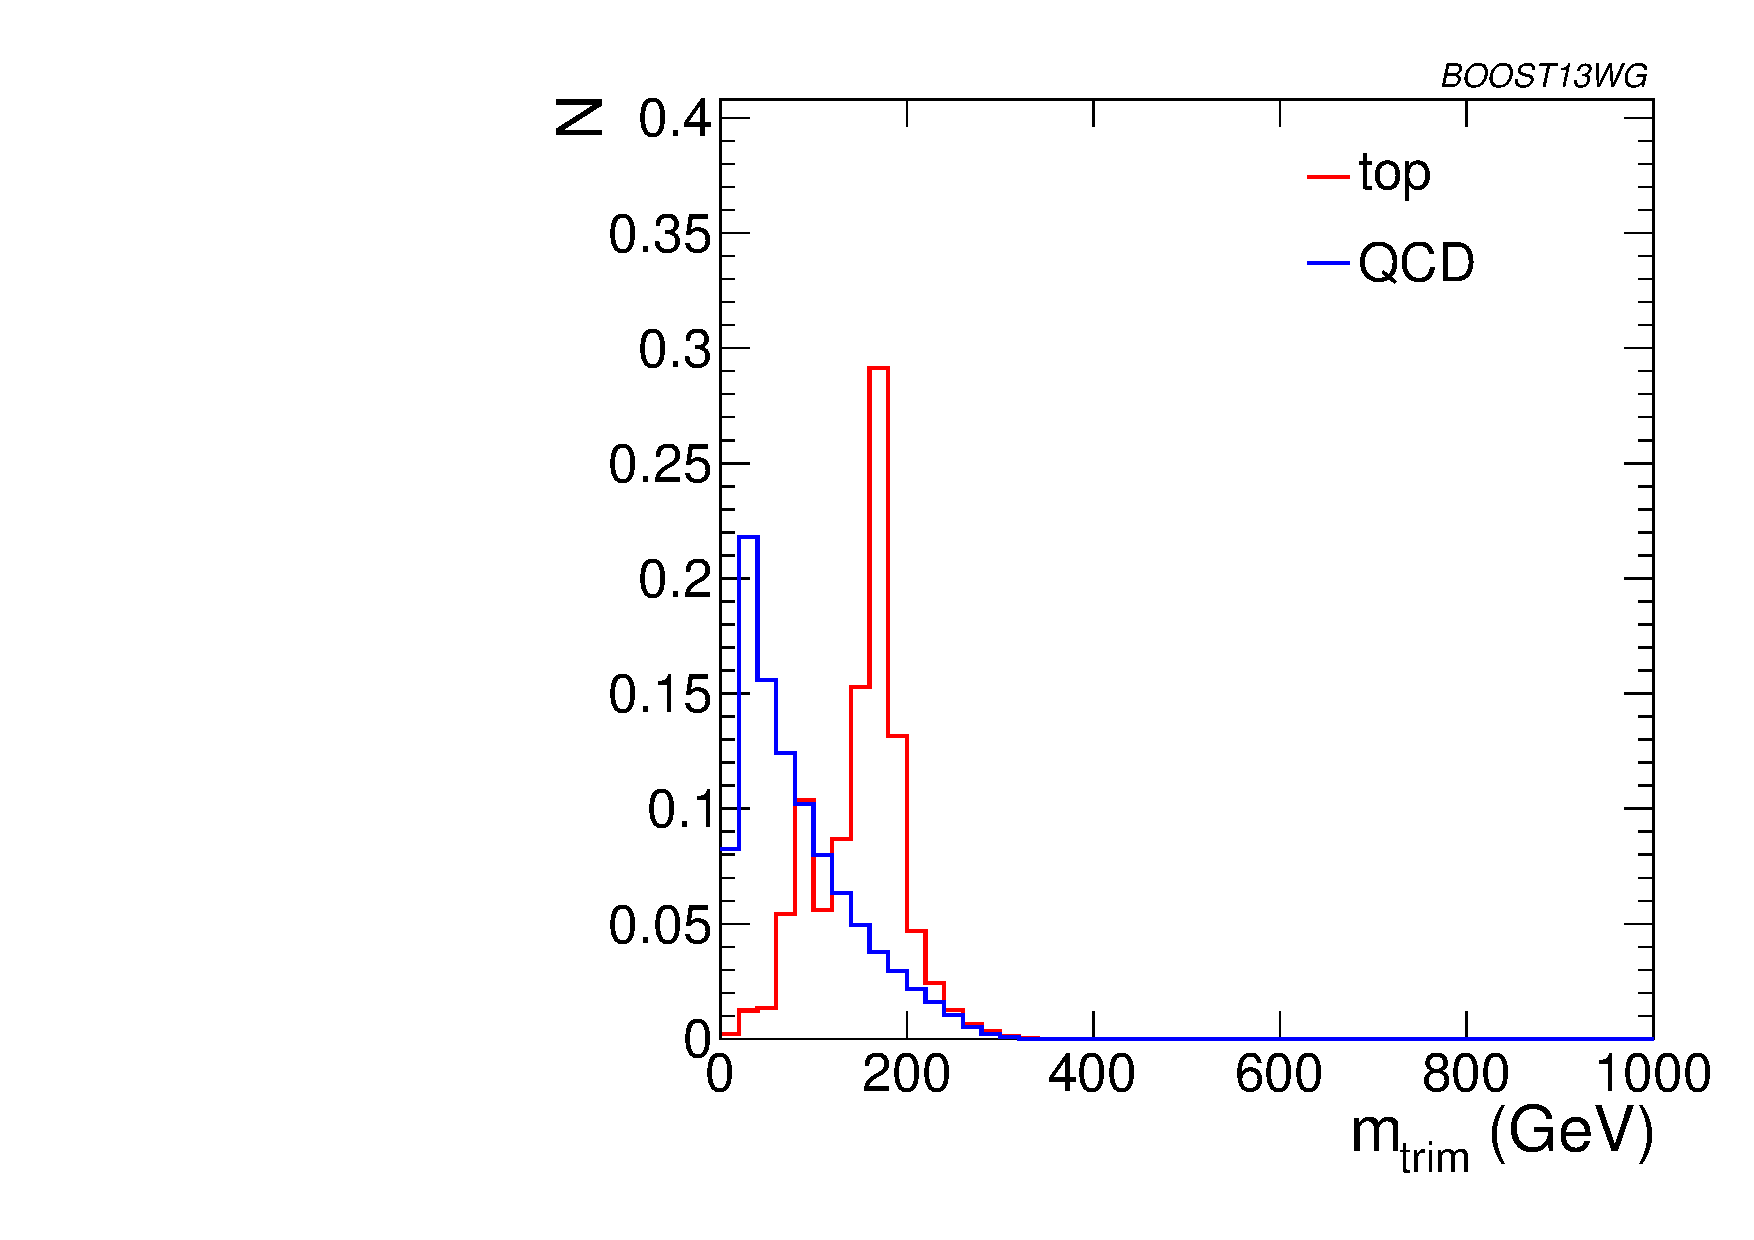
\includegraphics[width=0.245\textwidth]{./Figures/TTagging/single_variable/pT.600GeV.R.0.8/h_trim_pT_0_6.pdf}}
\subfigure[prune, $\pt=1.5-1.6$ TeV]{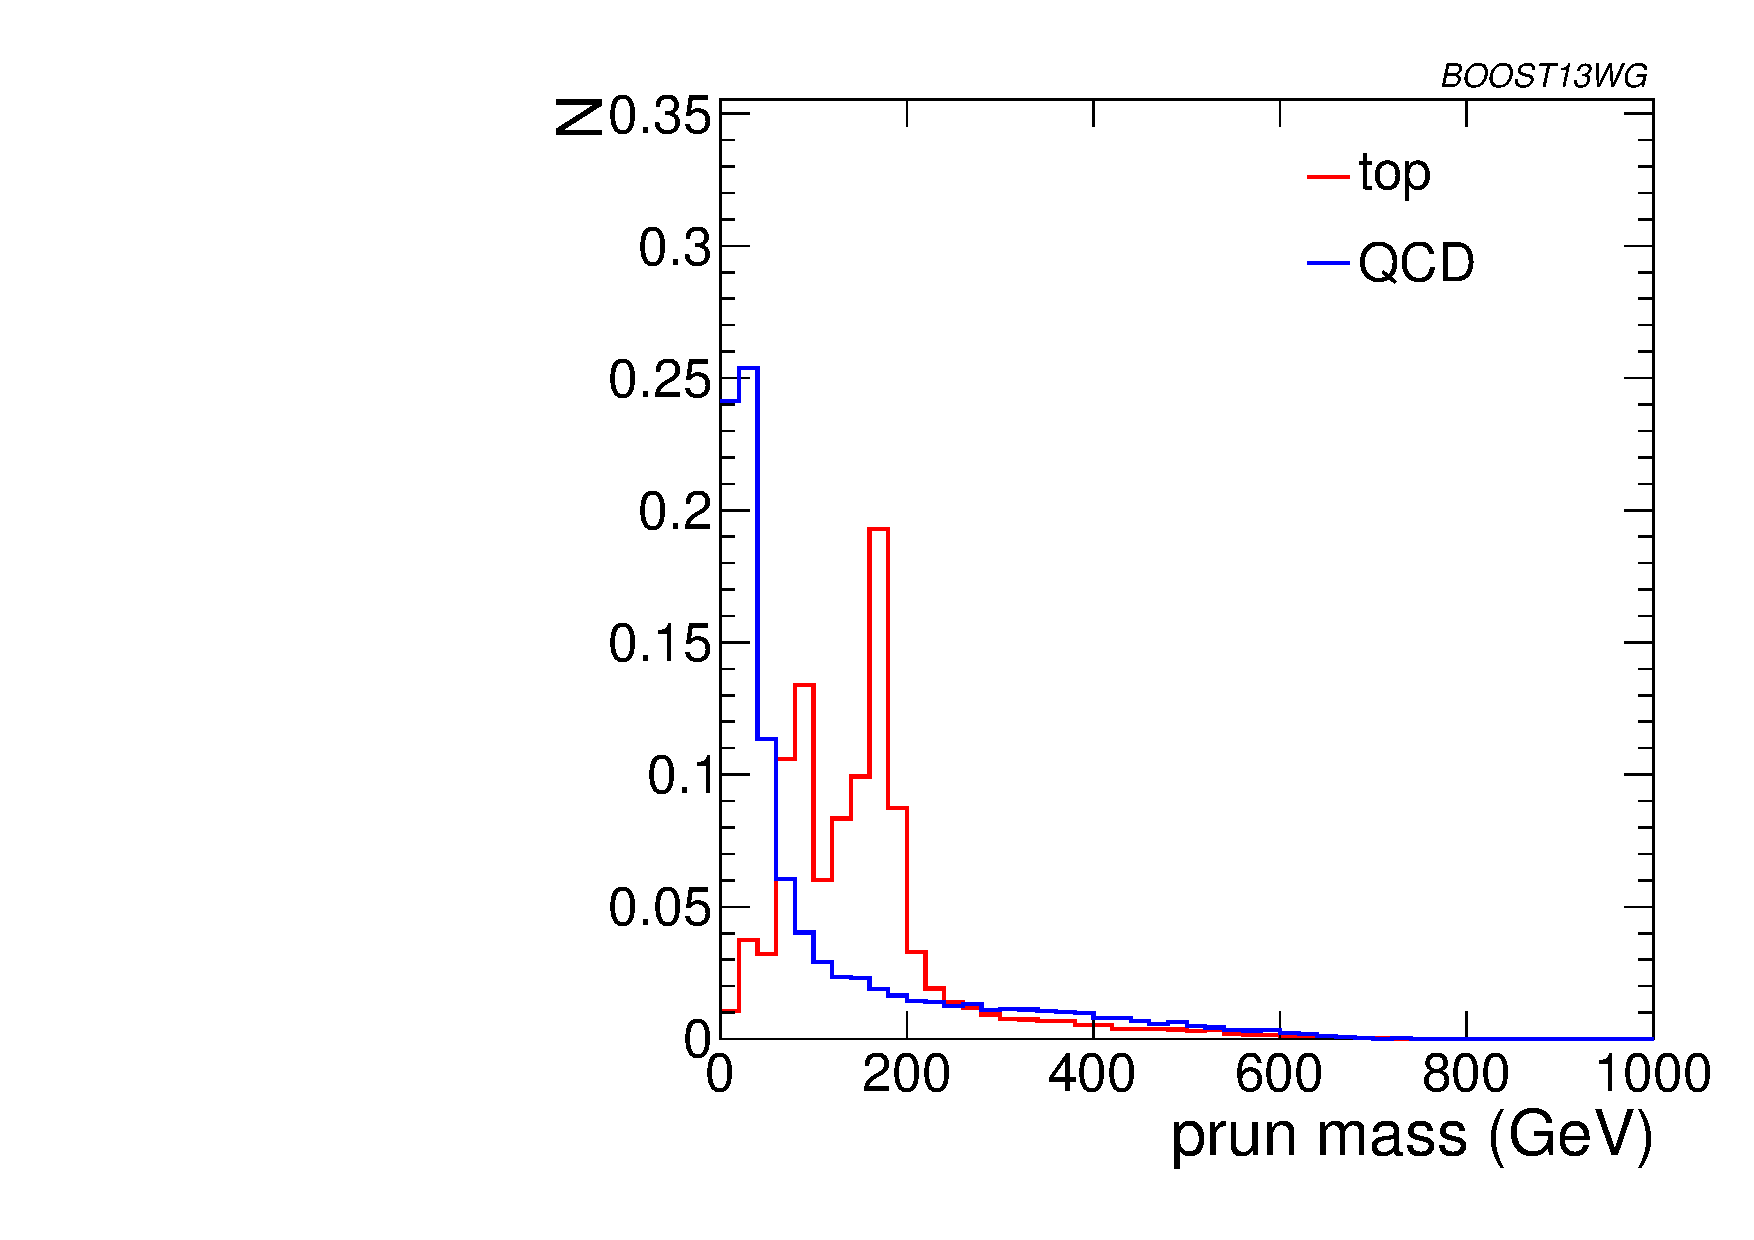
\includegraphics[width=0.245\textwidth]{./Figures/TTagging/single_variable/pT.1.5TeV.R.0.8/h_prun_pT_1_5.pdf}}
\subfigure[trim, $\pt=1.5-1.6$ TeV]{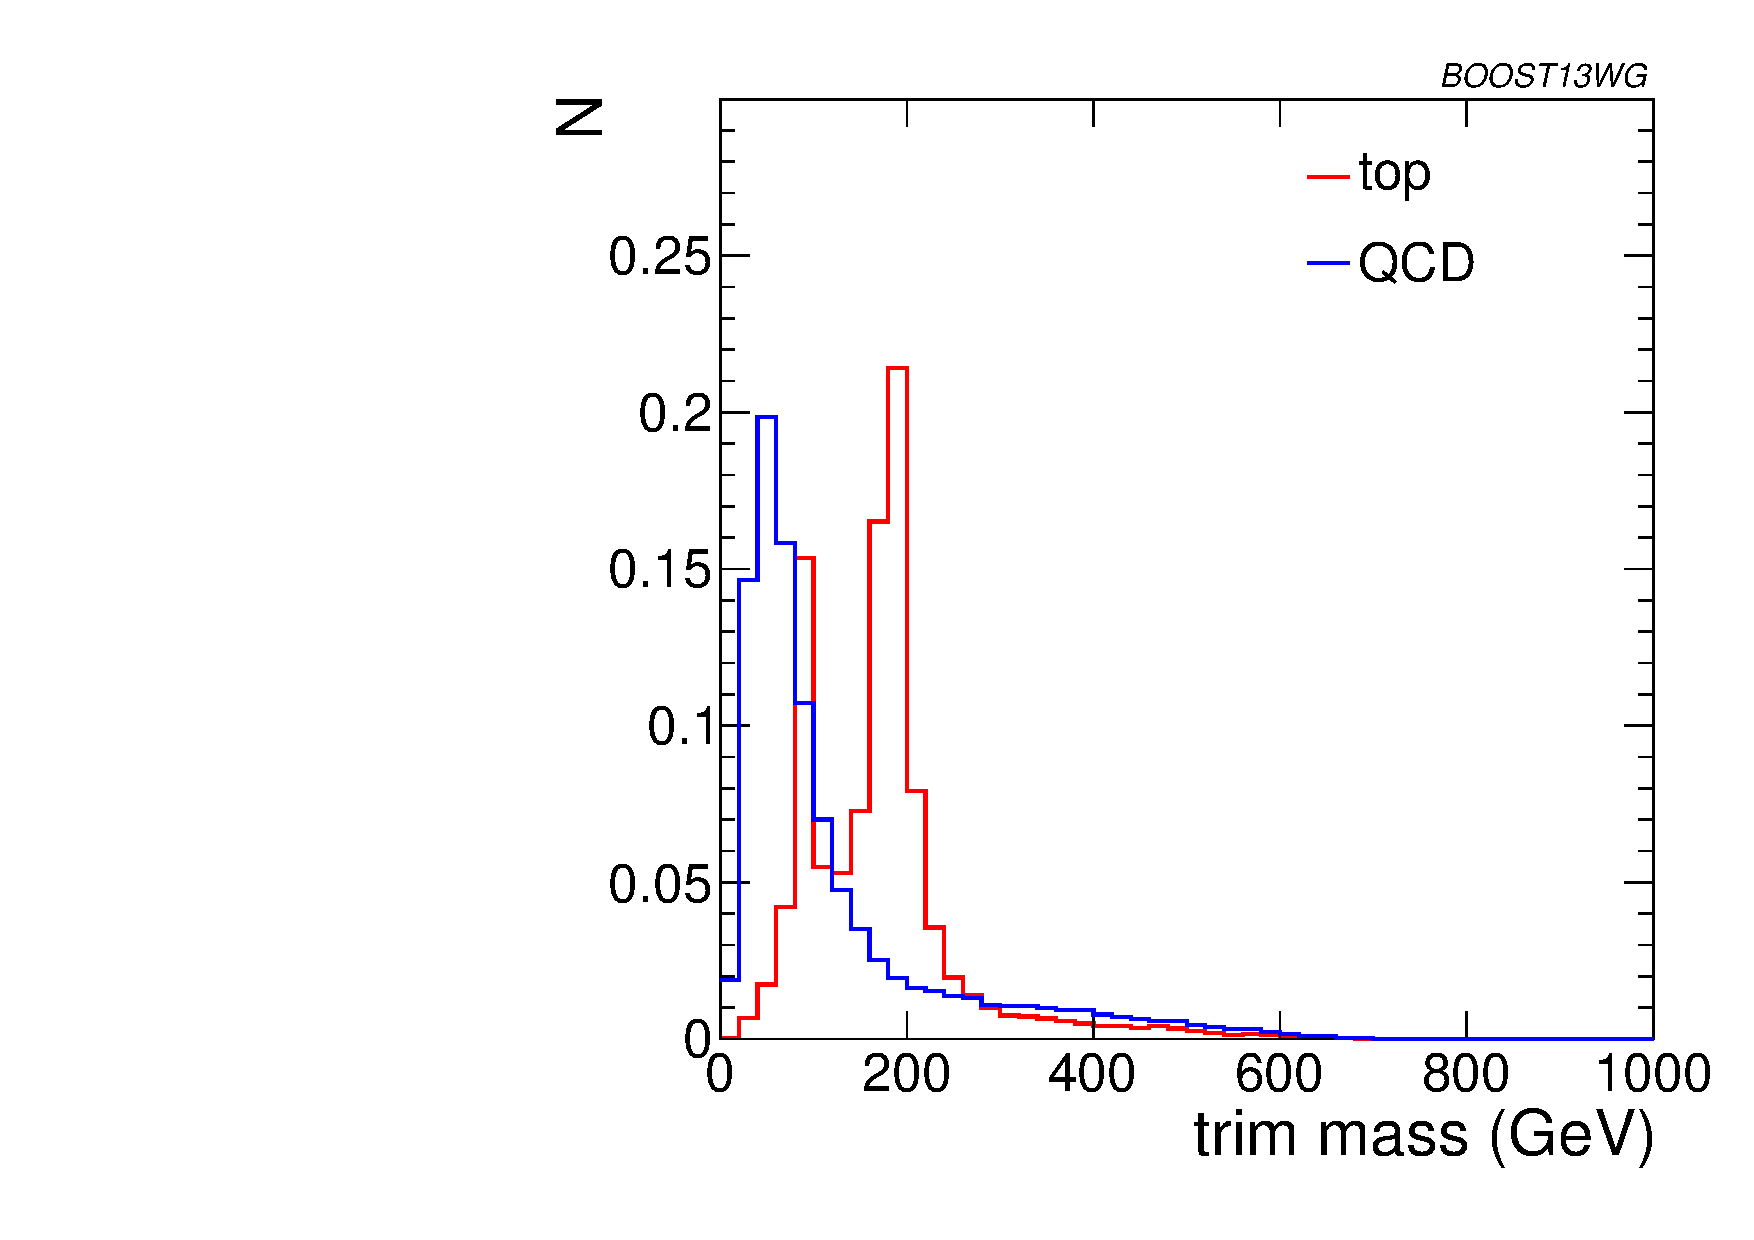
\includegraphics[width=0.245\textwidth]{./Figures/TTagging/single_variable/pT.1.5TeV.R.0.8/h_trim_pT_1_5.pdf}}
\caption{Comparison of top mass reconstruction with the Johns Hopkins (JH), HEPTopTaggers (HEP), pruning, and trimming at different $\pt$ using the anti-\kT algorithm, $R=0.8$. Each histogram is shown for the working point optimized for best performance with $m_t$ in the $0.3-0.35$ signal efficiency bin, and is normalized to the fraction of events passing the tagger.}
\label{fig:topmass_histogram_HEP_JH_pT}
\end{figure*}

We also see in Figure~\ref{fig:single_variable_ROC}(b) that the top mass from the JH tagger and the HEPTopTagger has superior performance relative to either of the grooming algorithms; this is because  the pruning and trimming algorithms do not have inherent $W$-identification steps and are not optimized for this purpose. Indeed, because of the lack of a $W$-identification step, grooming algorithms are forced to strike a balance between under-grooming the jet, which broadens the signal peak due to UE contamination and features a larger background rate, and over-grooming the jet, which occasionally throws out the $b$-jet and preserves only the $W$ components inside the jet. We demonstrate this effect in Figures~\ref{fig:topmass_histogram_HEP_JH} and \ref{fig:topmass_histogram_HEP_JH_pT}, showing that with $\varepsilon_{\rm sig}=0.3-0.35$, the optimal performance of the tagger over-grooms a substantial fraction of the jets ($\sim20-30\%$), leading to a spurious second peak at the $W$ mass. This effect is more pronounced at large $R$ and $\pt$, since more aggressive grooming is required in these limits to combat the increased contamination from UE and QCD radiation.

In Figures~\ref{fig:ptcomparison_singleshape_top} and~\ref{fig:ptcomparison_singletopmass_top} we directly compare ROC curves for jet shape observable performance and top mass performance respectively in the three different \pt bins considered whilst keeping the jet radius fixed at R=0.8. The input parameters of the taggers, groomers and shape variables are separately optimized in each \pt bin.  One can see from Figure~\ref{fig:ptcomparison_singleshape_top} that the tagging performance of jet shapes do not change substantially with $\pt$. The observables $\tau_{32}^{(\beta=1)}$ and Qjet volatility $\Gamma$ have the most variation and tend to degrade with higher $\pt$, as can be seen in Figure~\ref{fig:Qjet_comparison_pT}. This makes sense, as higher-$\pt$ QCD jets have more, harder emissions within the jet, giving rise to substructure that fakes the signal. By contrast, from Figure~\ref{fig:ptcomparison_singletopmass_top} we can see that most of the top mass observables have superior performance at higher $\pt$ due to the radiation from the top quark becoming more collimated. The notable exception is the HEPTopTagger, which degrades at higher $\pt$, likely in part due to the background-shaping effects discussed earlier.

%In Figure~\ref{fig:ptcomparison_singleshape_top} we directly compare ROC curves for jet shape observable performance in the three different \pt bins considered whilst keeping the jet radius fixed at R=0.8. The input parameters of the shape variables are separately optimized in each \pt bin.  One can see that the tagging performance of jet shapes do not change substantially with $\pt$. The observables $\tau_{32}^{(\beta=1)}$ and Qjet volatility $\Gamma$ have the most variation and tend to degrade with higher $\pt$, as can be seen in Figures~\ref{fig:Qjet_comparison_pT} and~\ref{fig:tau_comparison_pT}). This makes sense, as higher-$\pt$ QCD jets have more, harder emissions within the jet, giving rise to substructure that fakes the signal. 

%We also directly compare the performance of top mass and jet shape observables for different jet $\pt$ and radius. The input parameters of the taggers, groomers, and shape variables are separately optimized for each $\pt$ and radius:\\

%\noindent{\bf $\pt$ comparison:} We compare various top tagging observables for jets in different $\pt$ bins and $R=0.8$ in Figs.~\ref{fig:ptcomparison_singleshape_top} and \ref{fig:ptcomparison_singletopmass_top}. The tagging performance of jet shapes do not change substantially with $\pt$. $\tau_{32}^{(\beta=1)}$ and the Qjet volatility $\Gamma$ have the most variation and tend to degrade with higher $\pt$ (see Fig.~\ref{fig:Qjet_comparison_pT}-\ref{fig:tau_comparison_pT}). This makes sense, as higher-$\pt$ QCD jets have more, harder emissions within the jet, giving rise to substructure that fakes the signal. By contrast, most of the top mass observables have superior performance at higher $\pt$ due to the radiation from the top quark becoming more collimated. The notable exception is the HEPTopTagger, which degrades at higher $\pt$, likely in part due to the background-shaping effects discussed earlier.\\

\begin{figure*}
\centering
\subfigure[$C_2^{(\beta=1)}$]{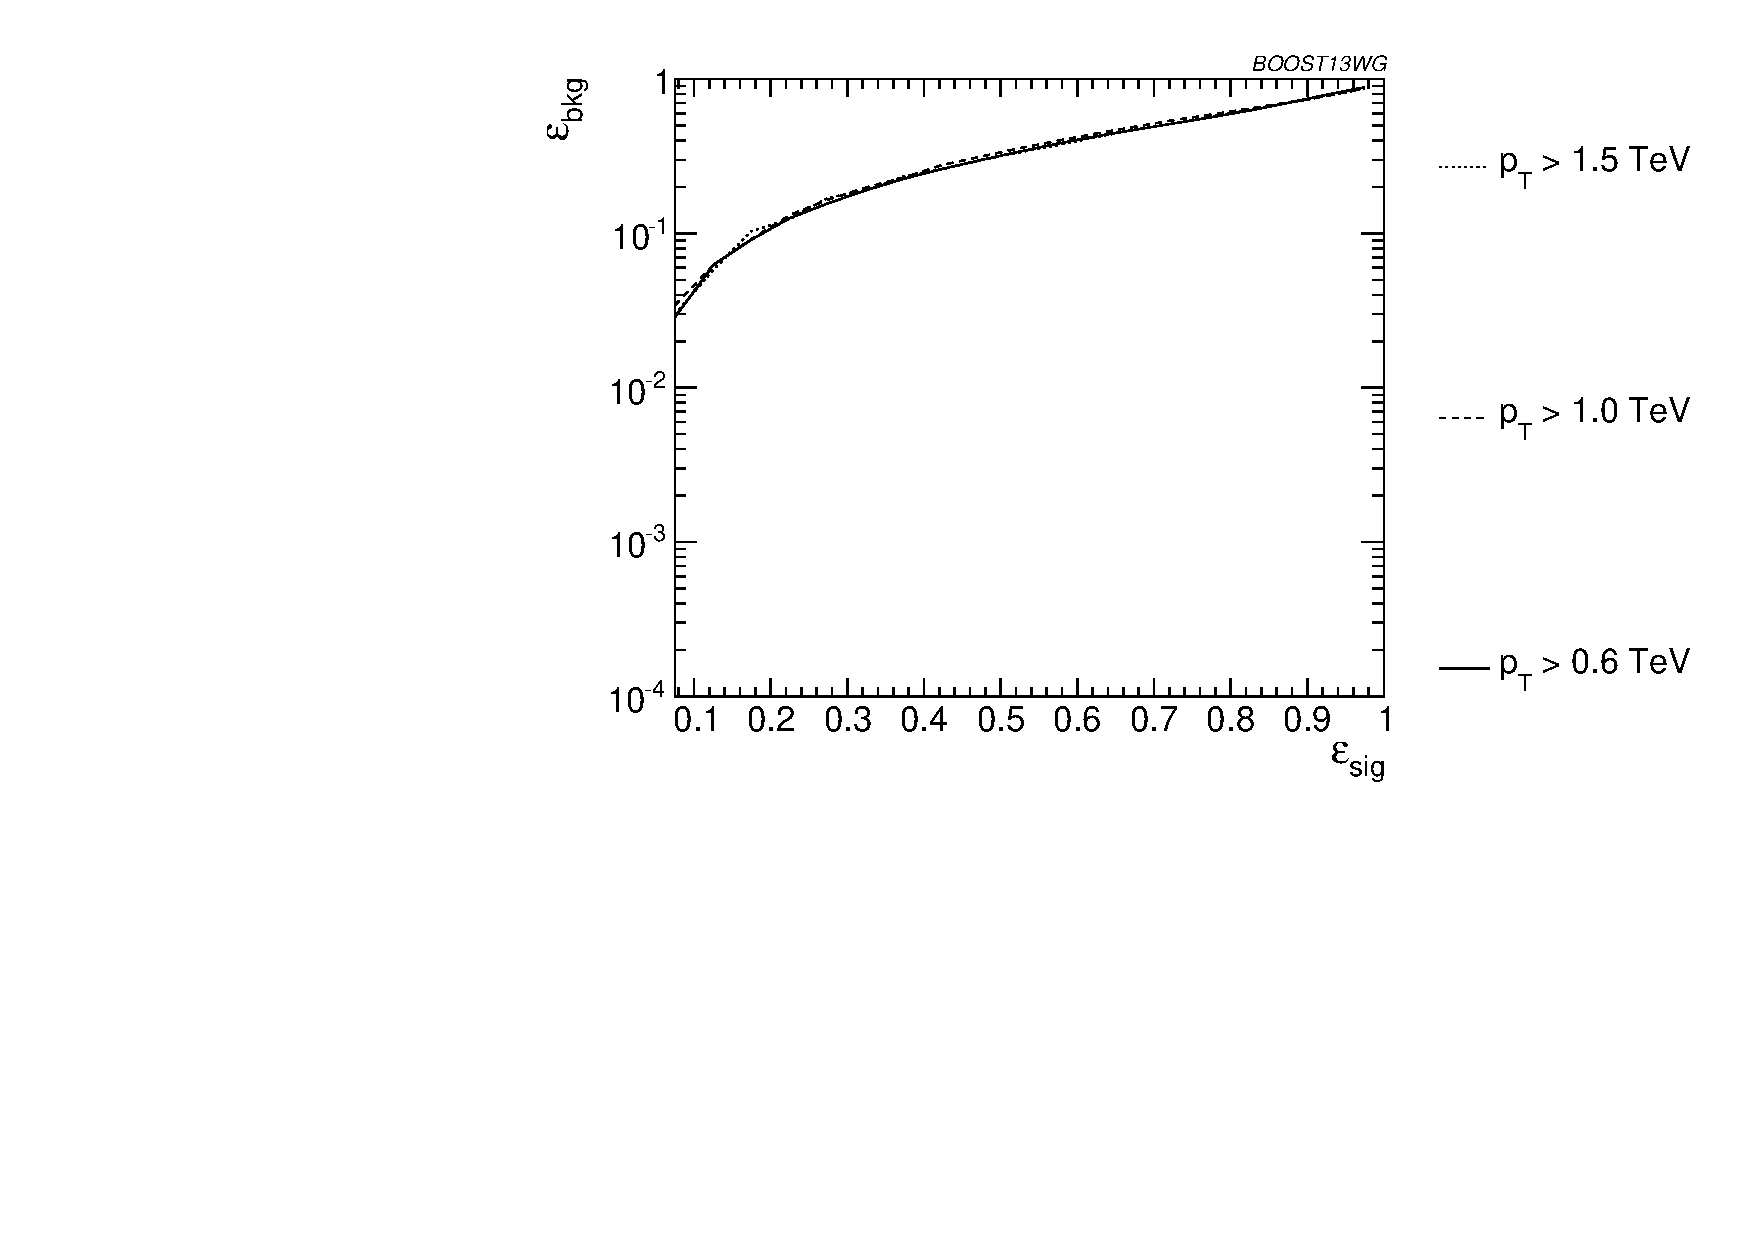
\includegraphics[width=0.48\textwidth]{./Figures/TTagging/single_variable/pT_compare/Rocs_C2b1_pTcompare.pdf}}
\subfigure[$C_3^{(\beta=1)}$]{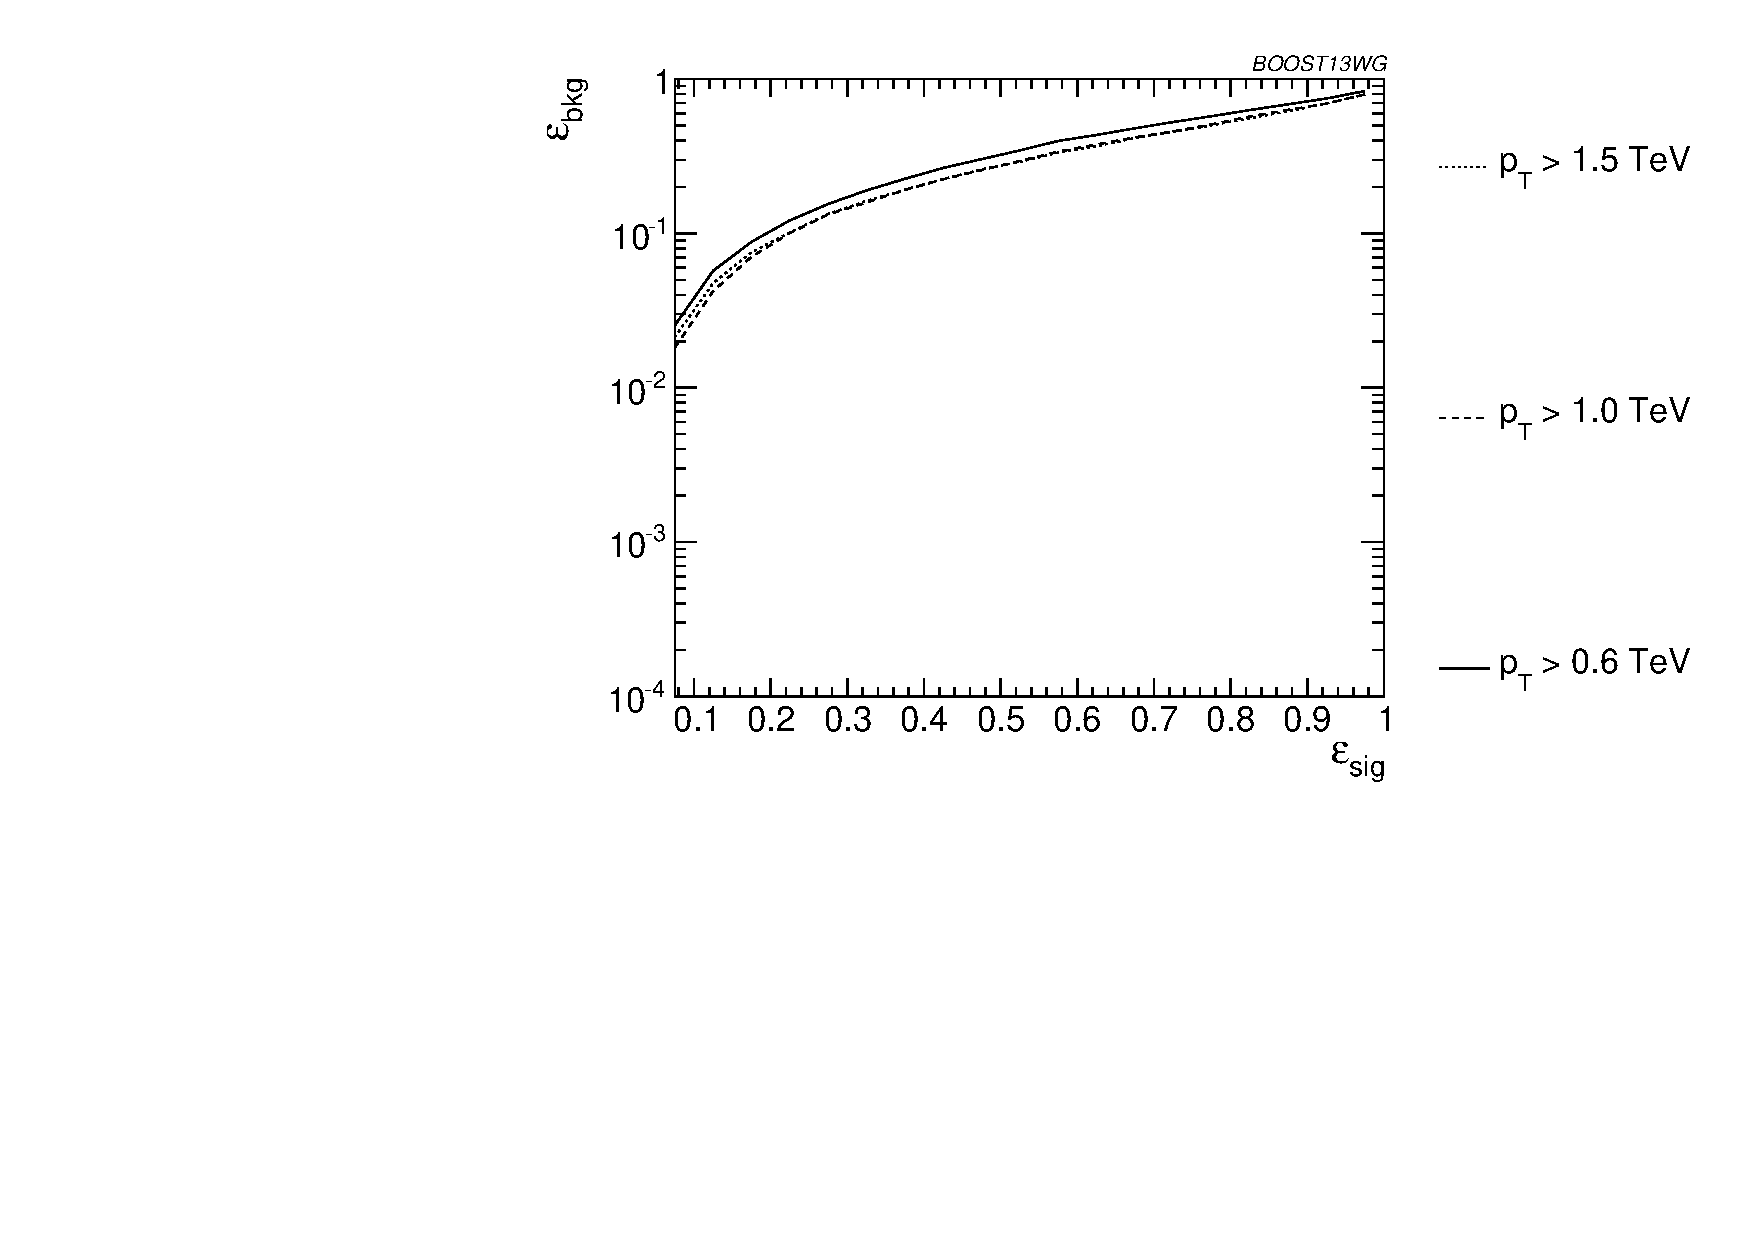
\includegraphics[width=0.48\textwidth]{./Figures/TTagging/single_variable/pT_compare/Rocs_C3b1_pTcompare.pdf}\label{fig:ptcomparison_singleshape_top_C3}}
\subfigure[$\tau_{21}^{(\beta=1)}$]{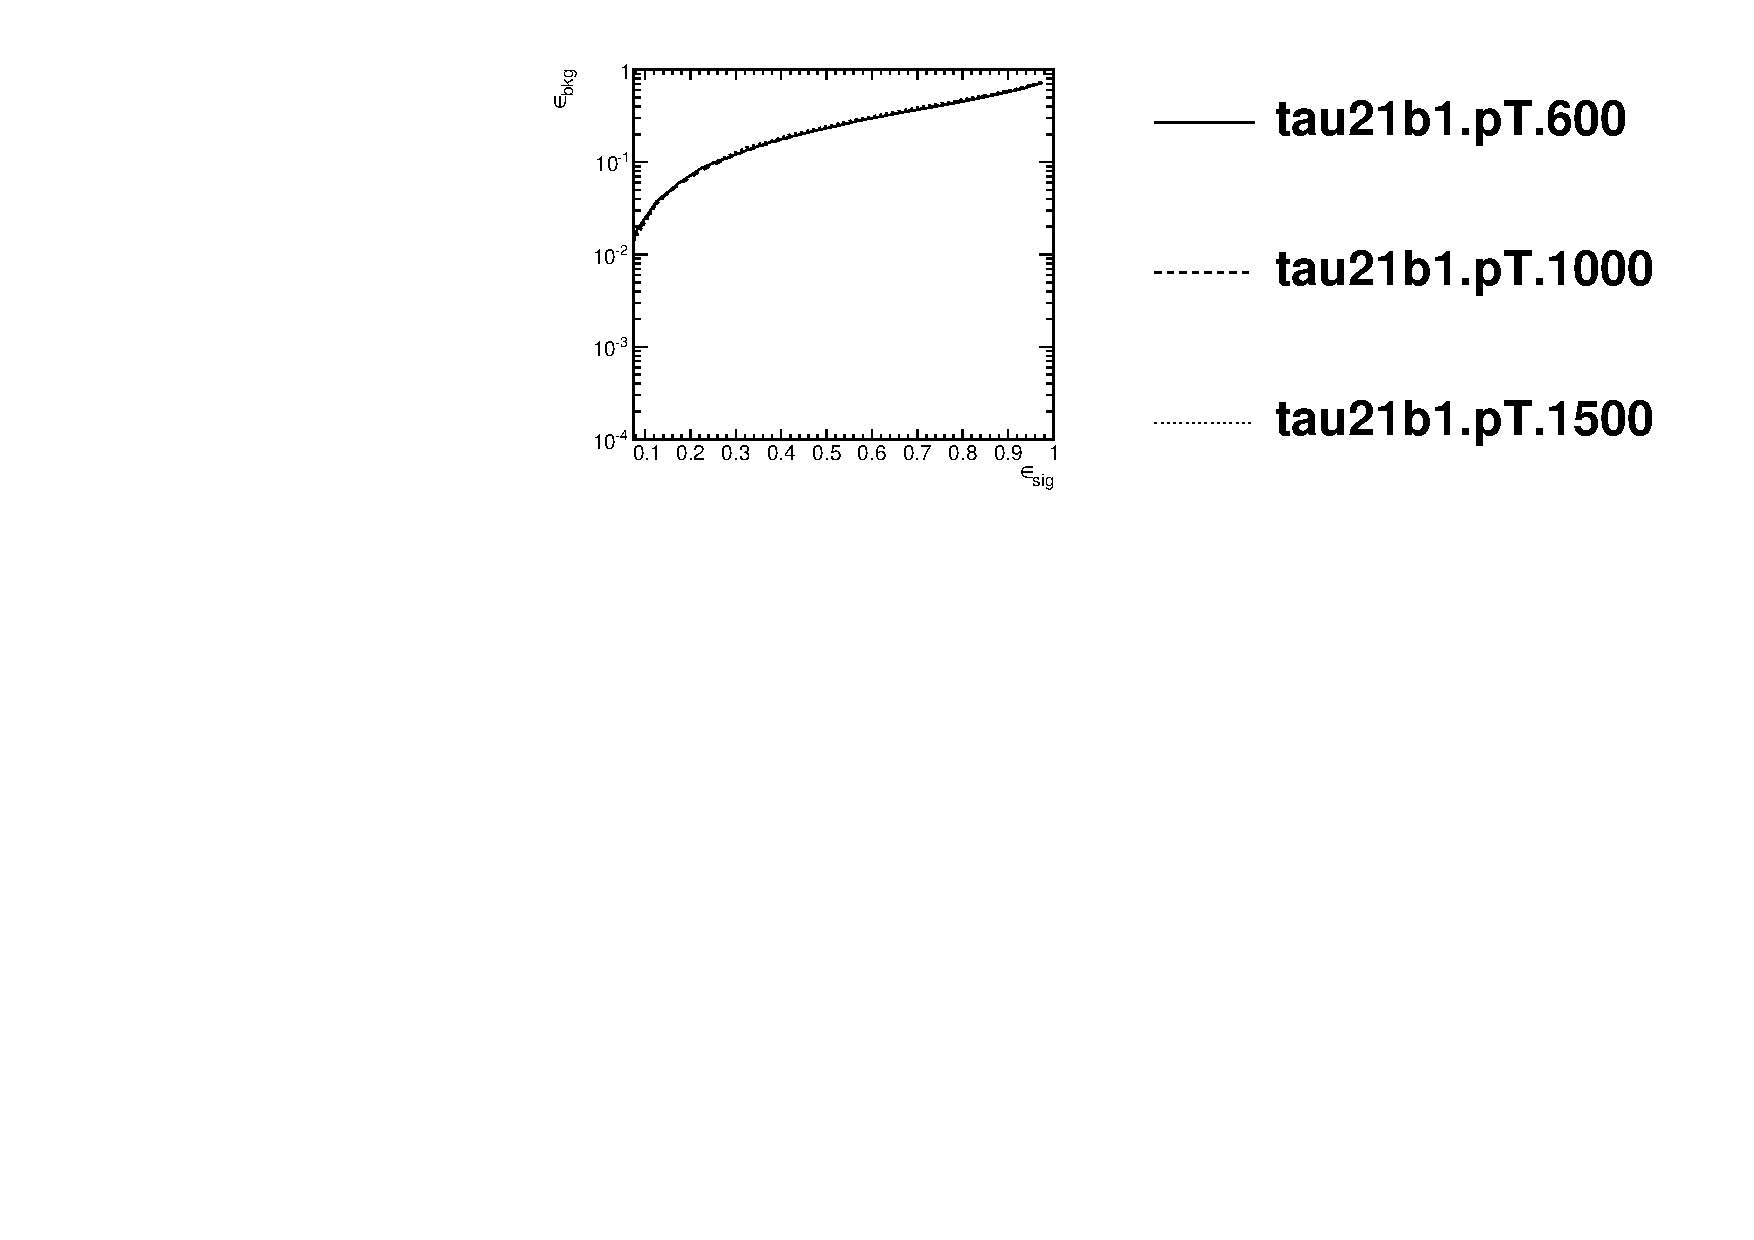
\includegraphics[width=0.48\textwidth]{./Figures/TTagging/single_variable/pT_compare/Rocs_tau21b1_pTcompare.pdf}}
\subfigure[$\tau_{32}^{(\beta=1)}$]{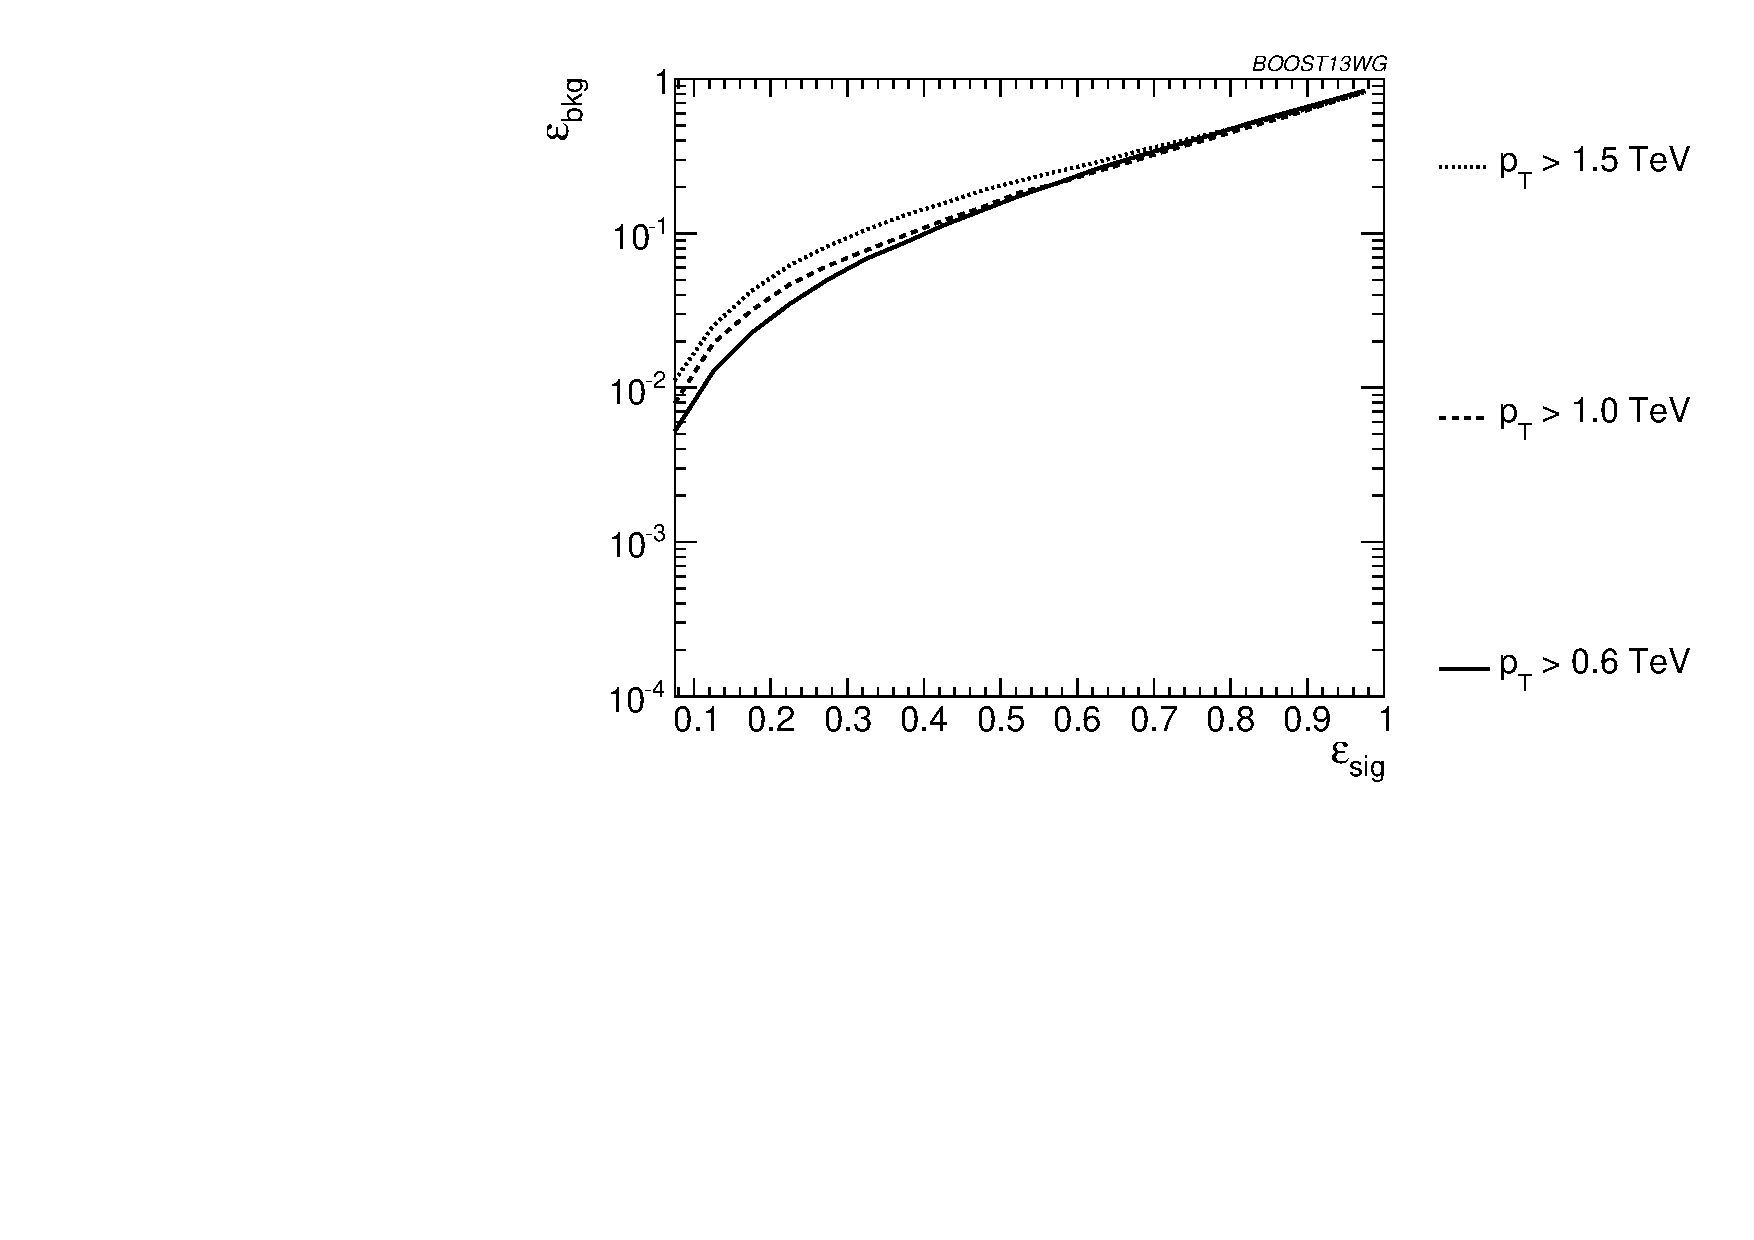
\includegraphics[width=0.48\textwidth]{./Figures/TTagging/single_variable/pT_compare/Rocs_tau32b1_pTcompare.pdf}}
\subfigure[Qjet mass volatility]{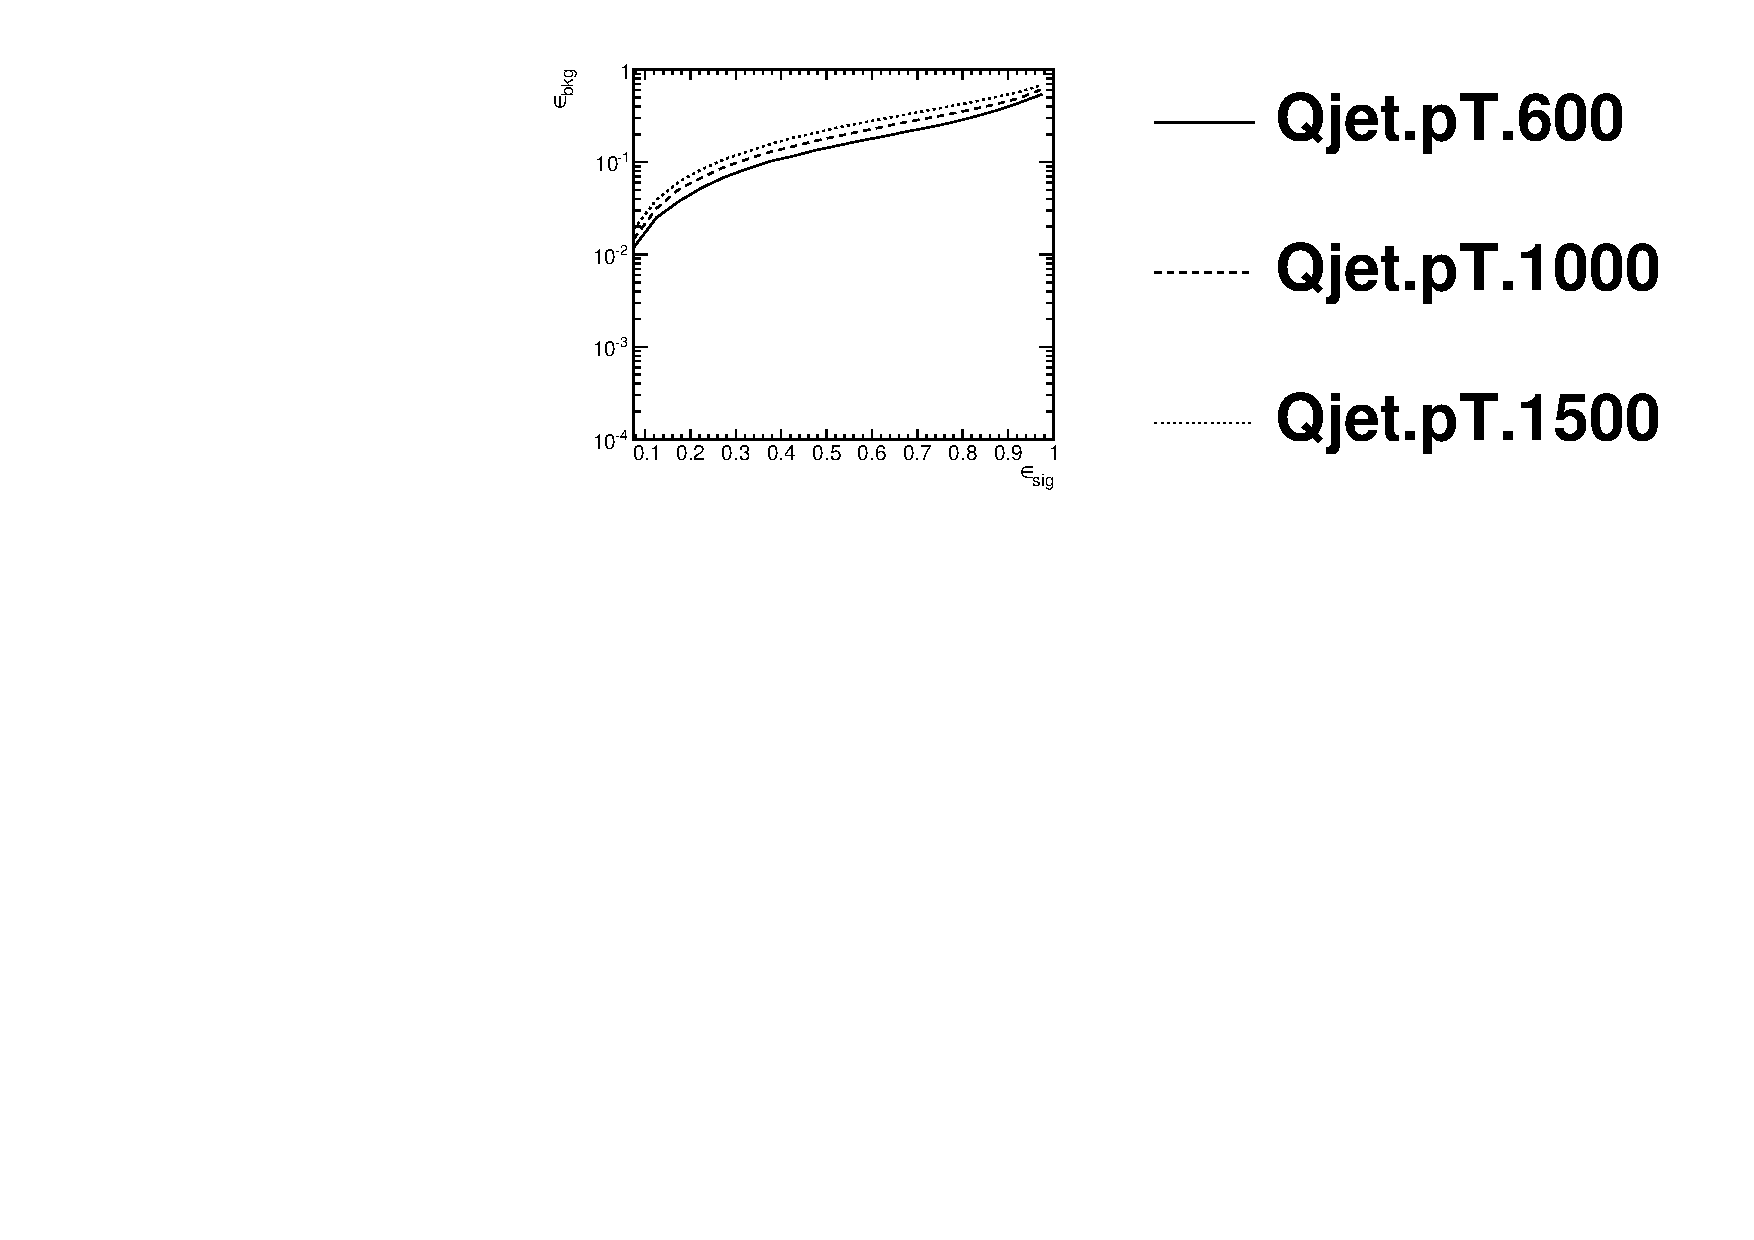
\includegraphics[width=0.48\textwidth]{./Figures/TTagging/single_variable/pT_compare/Rocs_Qjet_pTcompare.pdf}}
\caption{Comparison of individual jet shape performance at different \pt using the anti-\kT R=0.8 algorithm.}
\label{fig:ptcomparison_singleshape_top}
\end{figure*}

%\begin{figure*}
%\centering
%\subfigure[$C_2^{(\beta=1)}$, $\pt=600-700$ GeV]{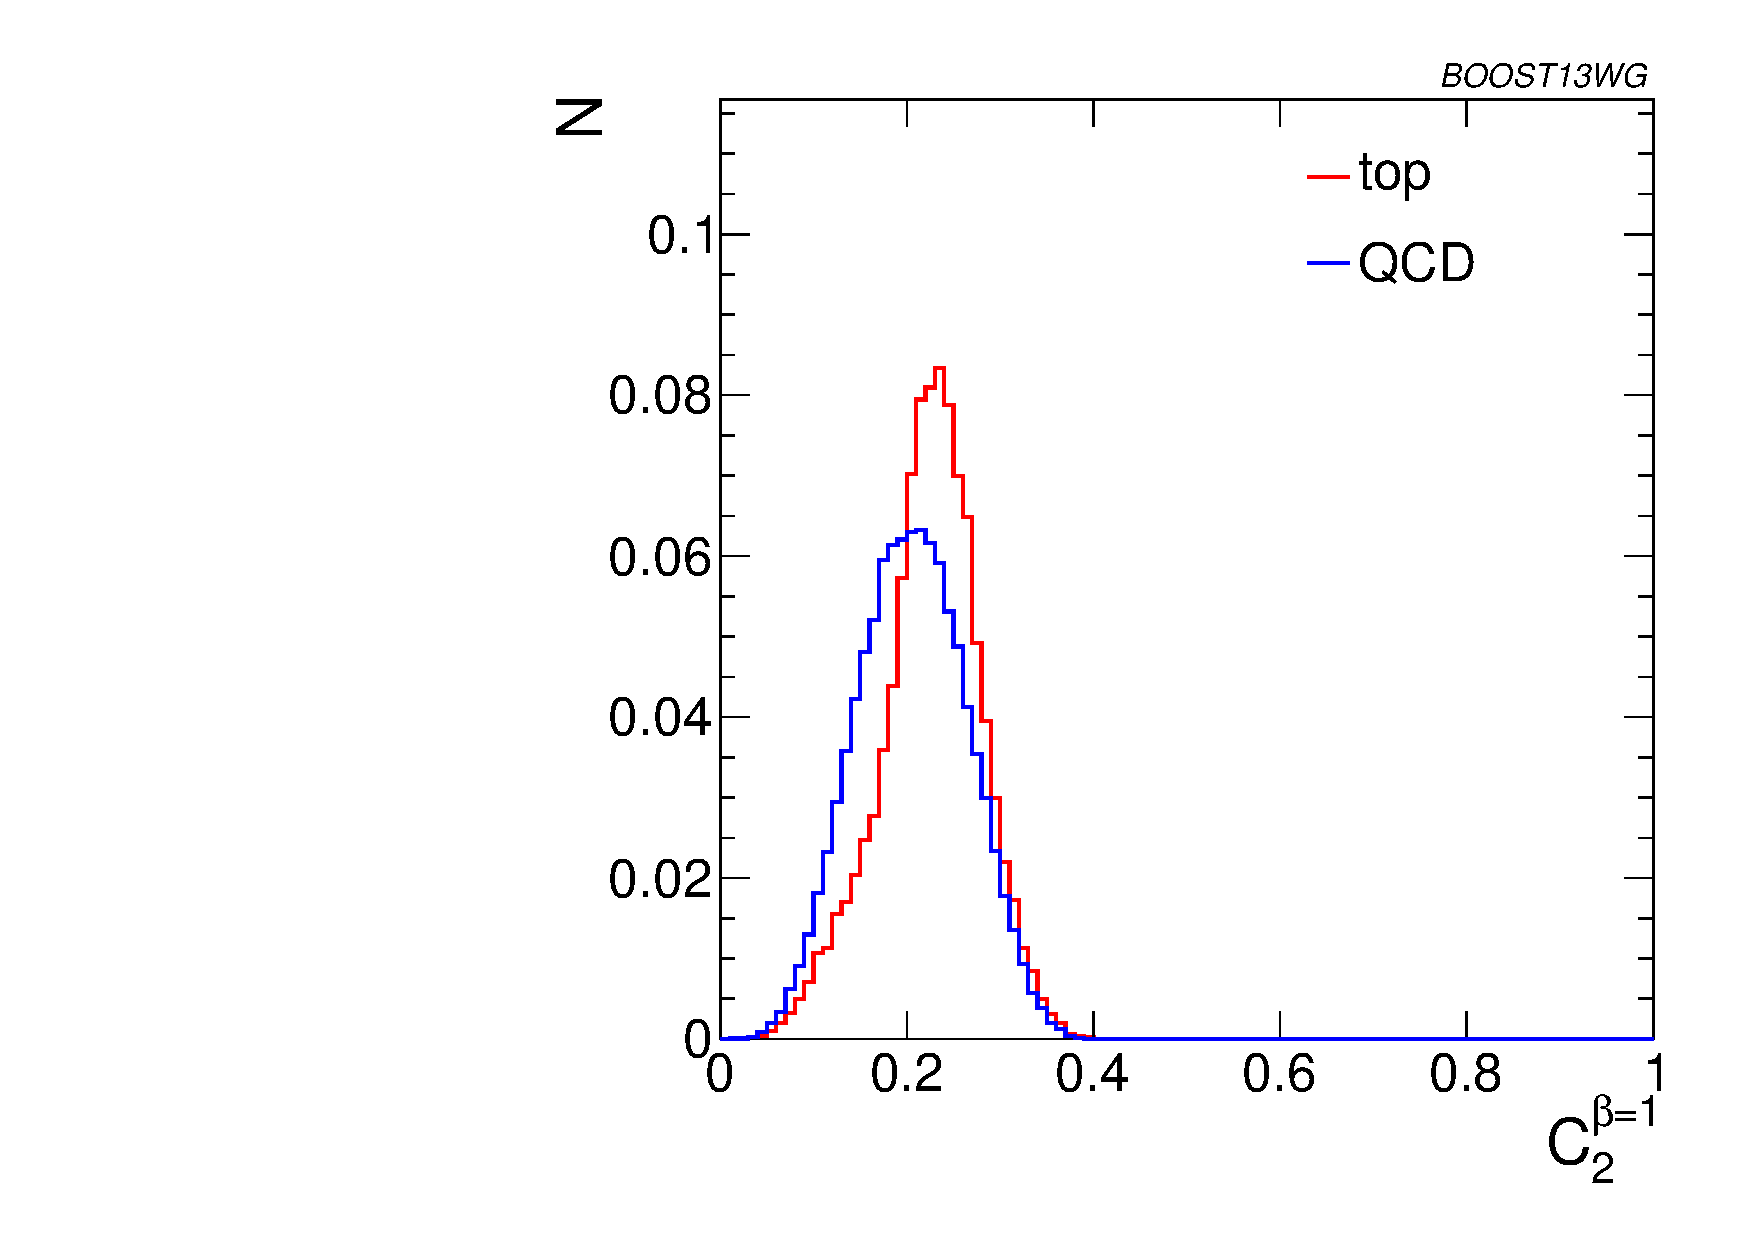
\includegraphics[width=0.32\textwidth]{./Figures/TTagging/single_variable/pT.600GeV.R.0.8/h_C2B1_pT_0_6.pdf}}
%\subfigure[$C_2^{(\beta=1)}$, $\pt=1-1.1$ TeV]{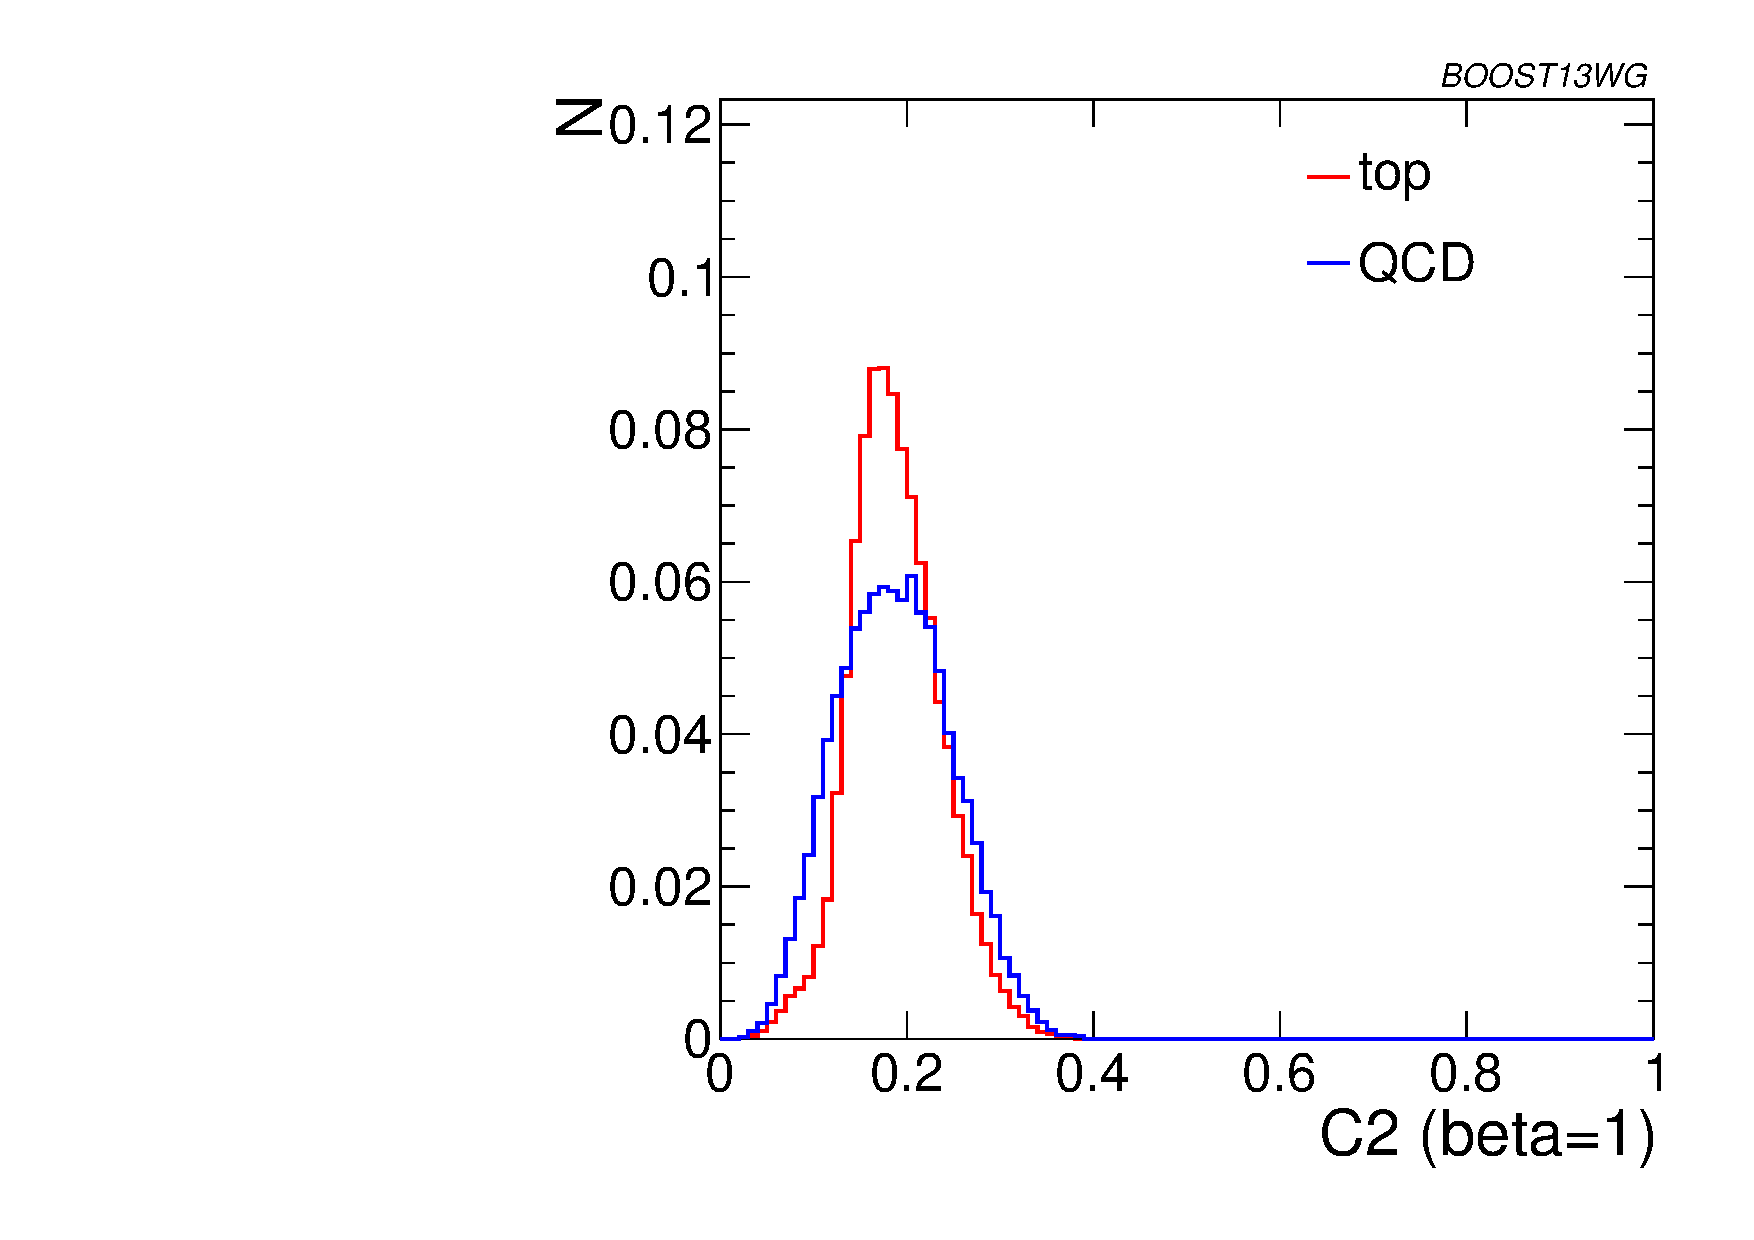
\includegraphics[width=0.32\textwidth]{./Figures/TTagging/single_variable/pT.1TeV.R.0.8/h_C2B1_pT_1_0.pdf}}
%\subfigure[$C_2^{(\beta=1)}$, $\pt=1.5-1.6$ TeV]{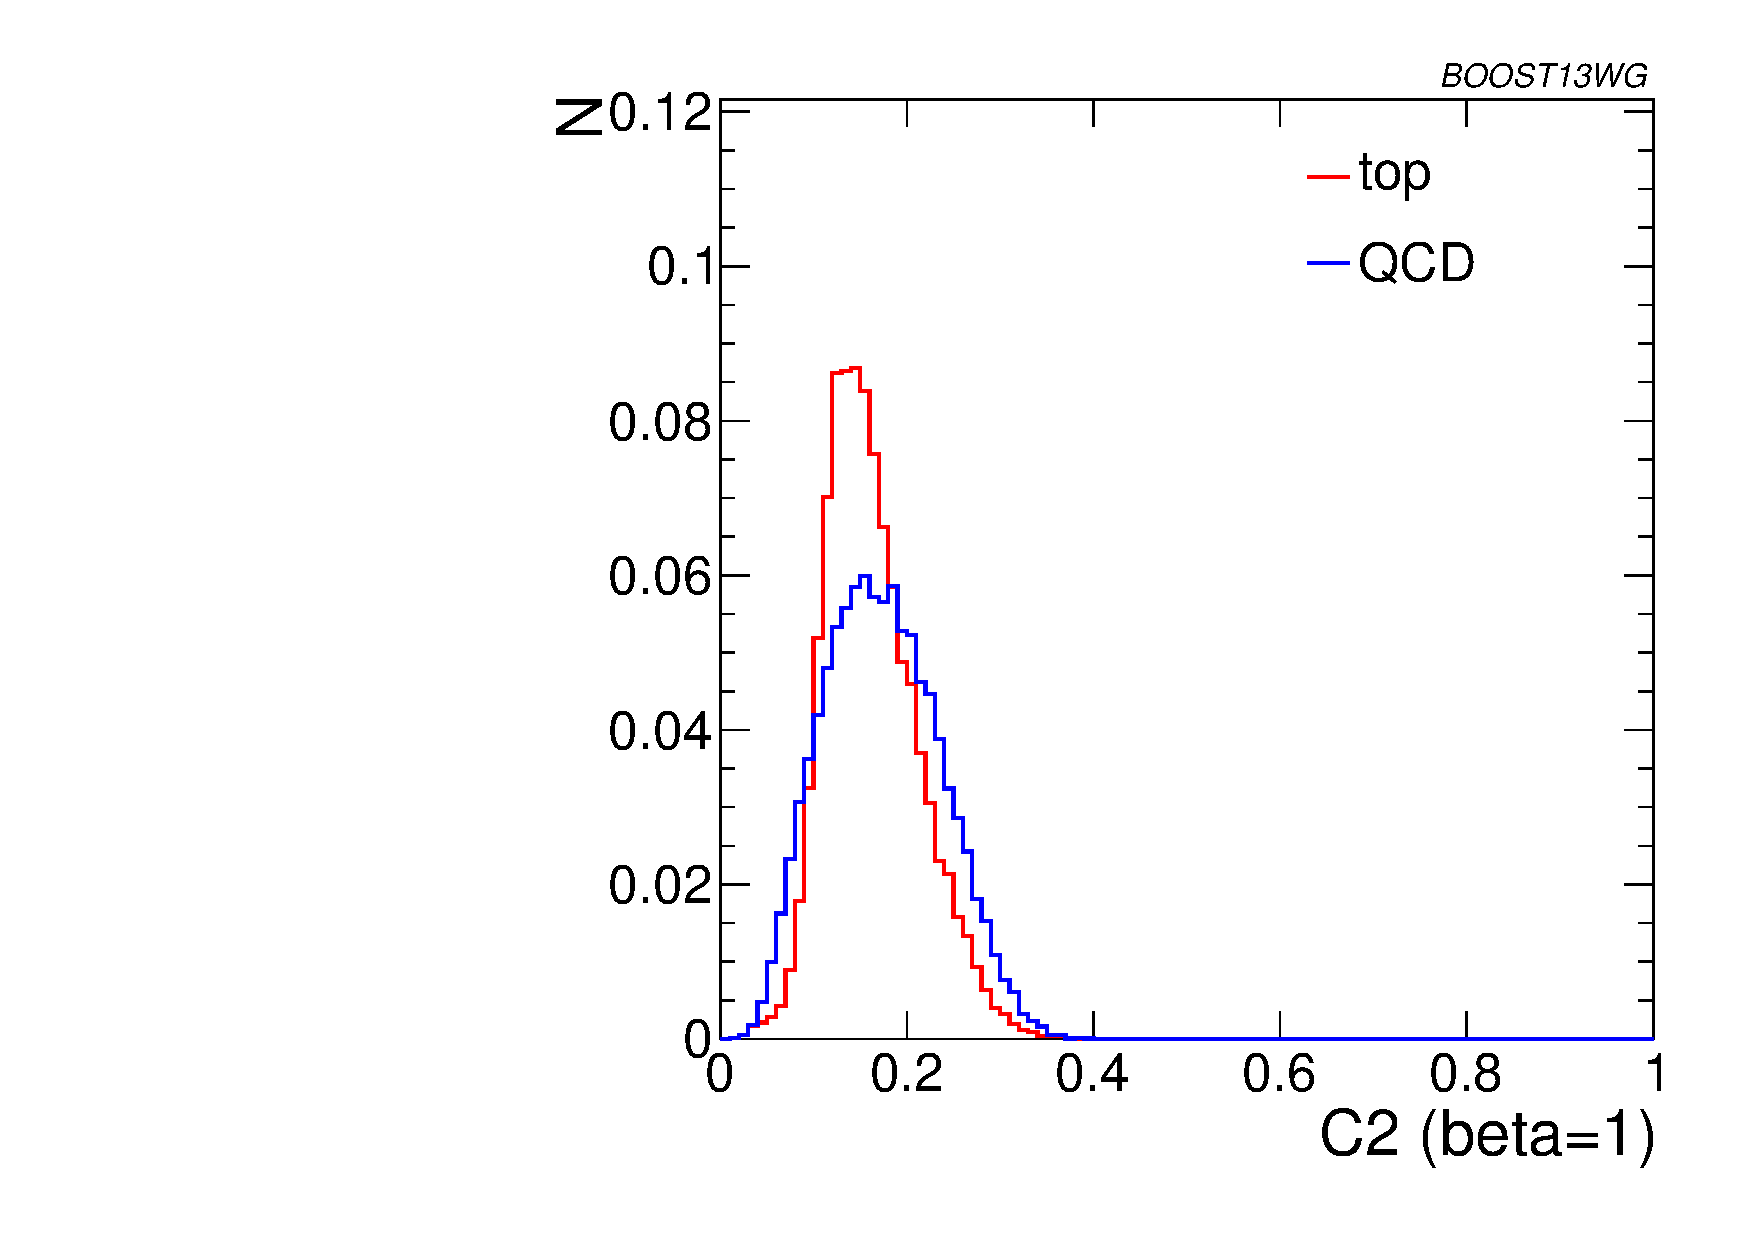
\includegraphics[width=0.32\textwidth]{./Figures/TTagging/single_variable/pT.1.5TeV.R.0.8/h_C2B1_R_0_8.pdf}}
%\subfigure[$C_3^{(\beta=1)}$, $\pt=600-700$ GeV]{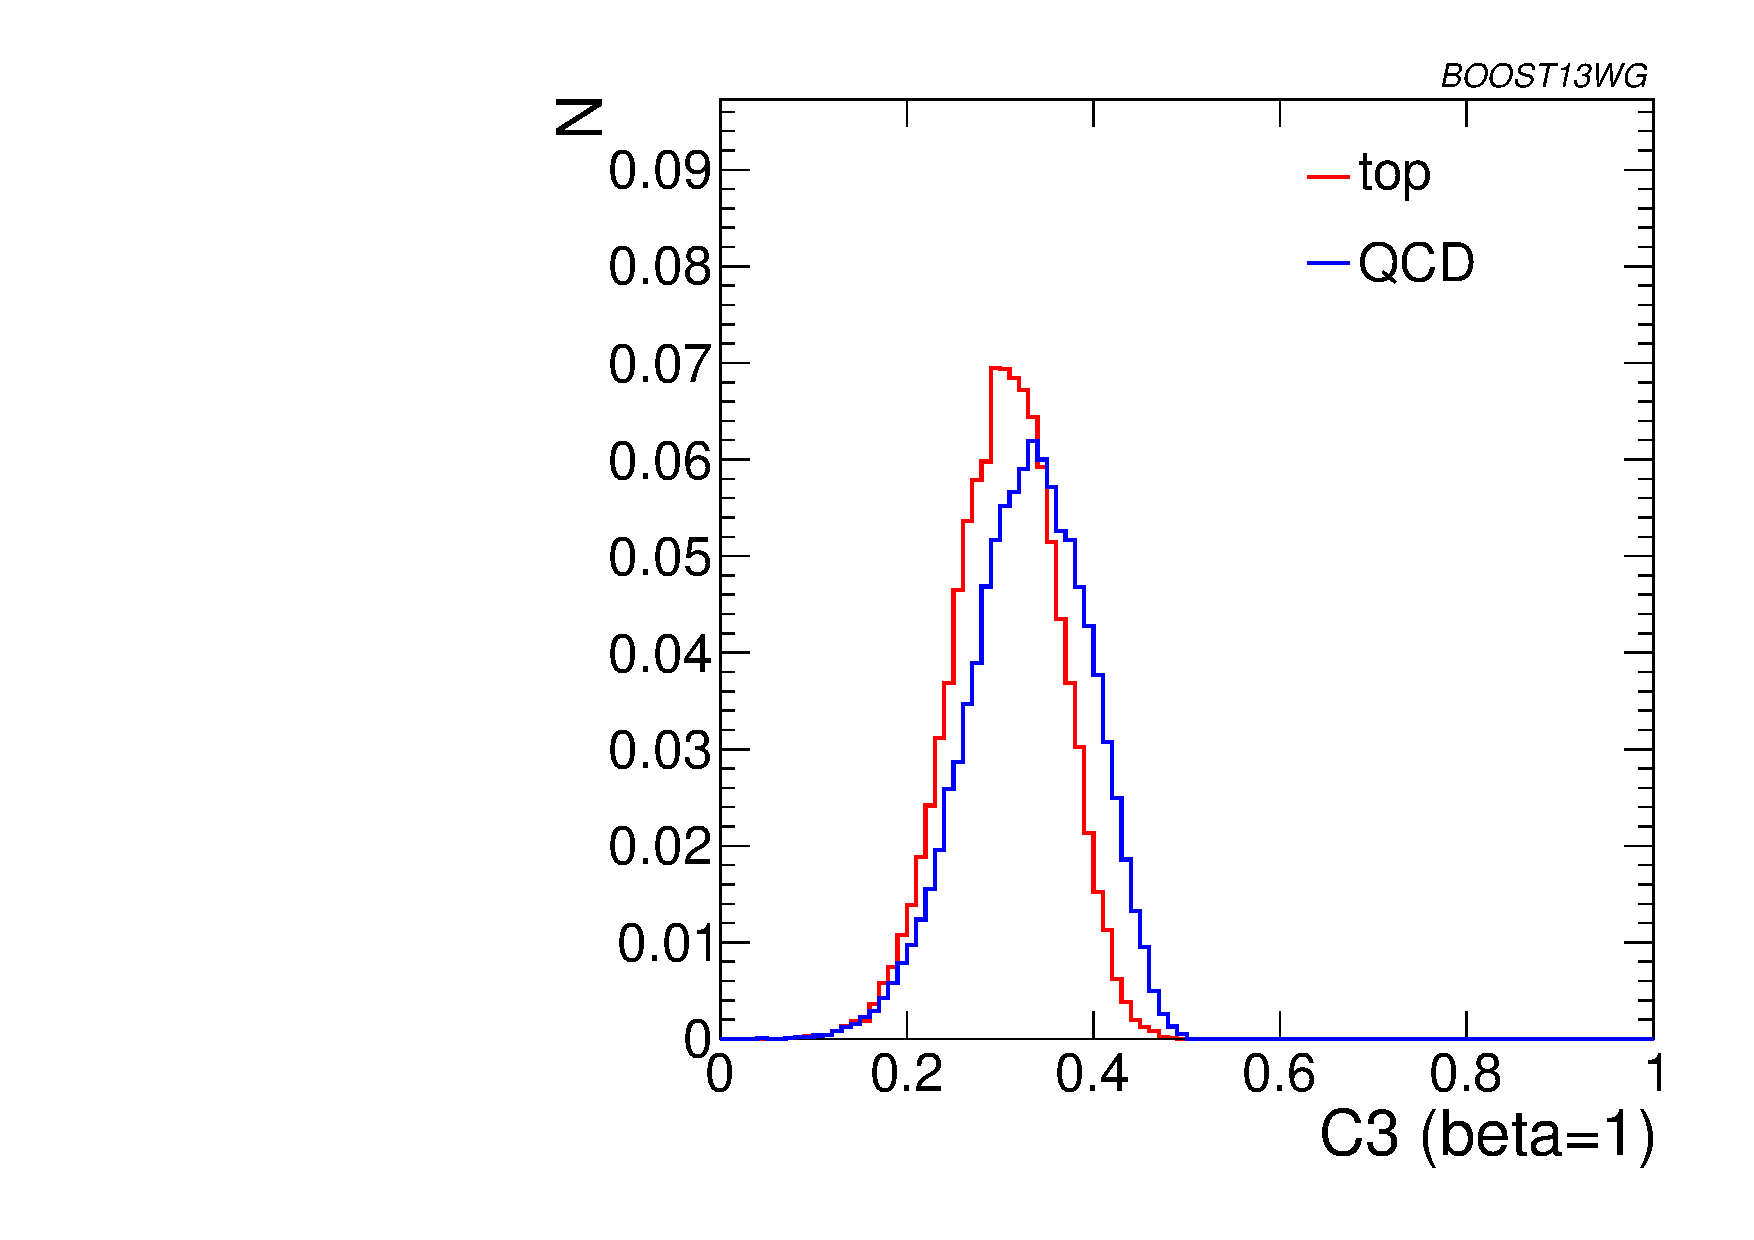
\includegraphics[width=0.32\textwidth]{./Figures/TTagging/single_variable/pT.600GeV.R.0.8/h_C3B1_pT_0_6.pdf}}
%\subfigure[$C_3^{(\beta=1)}$, $\pt=1-1.1$ TeV]{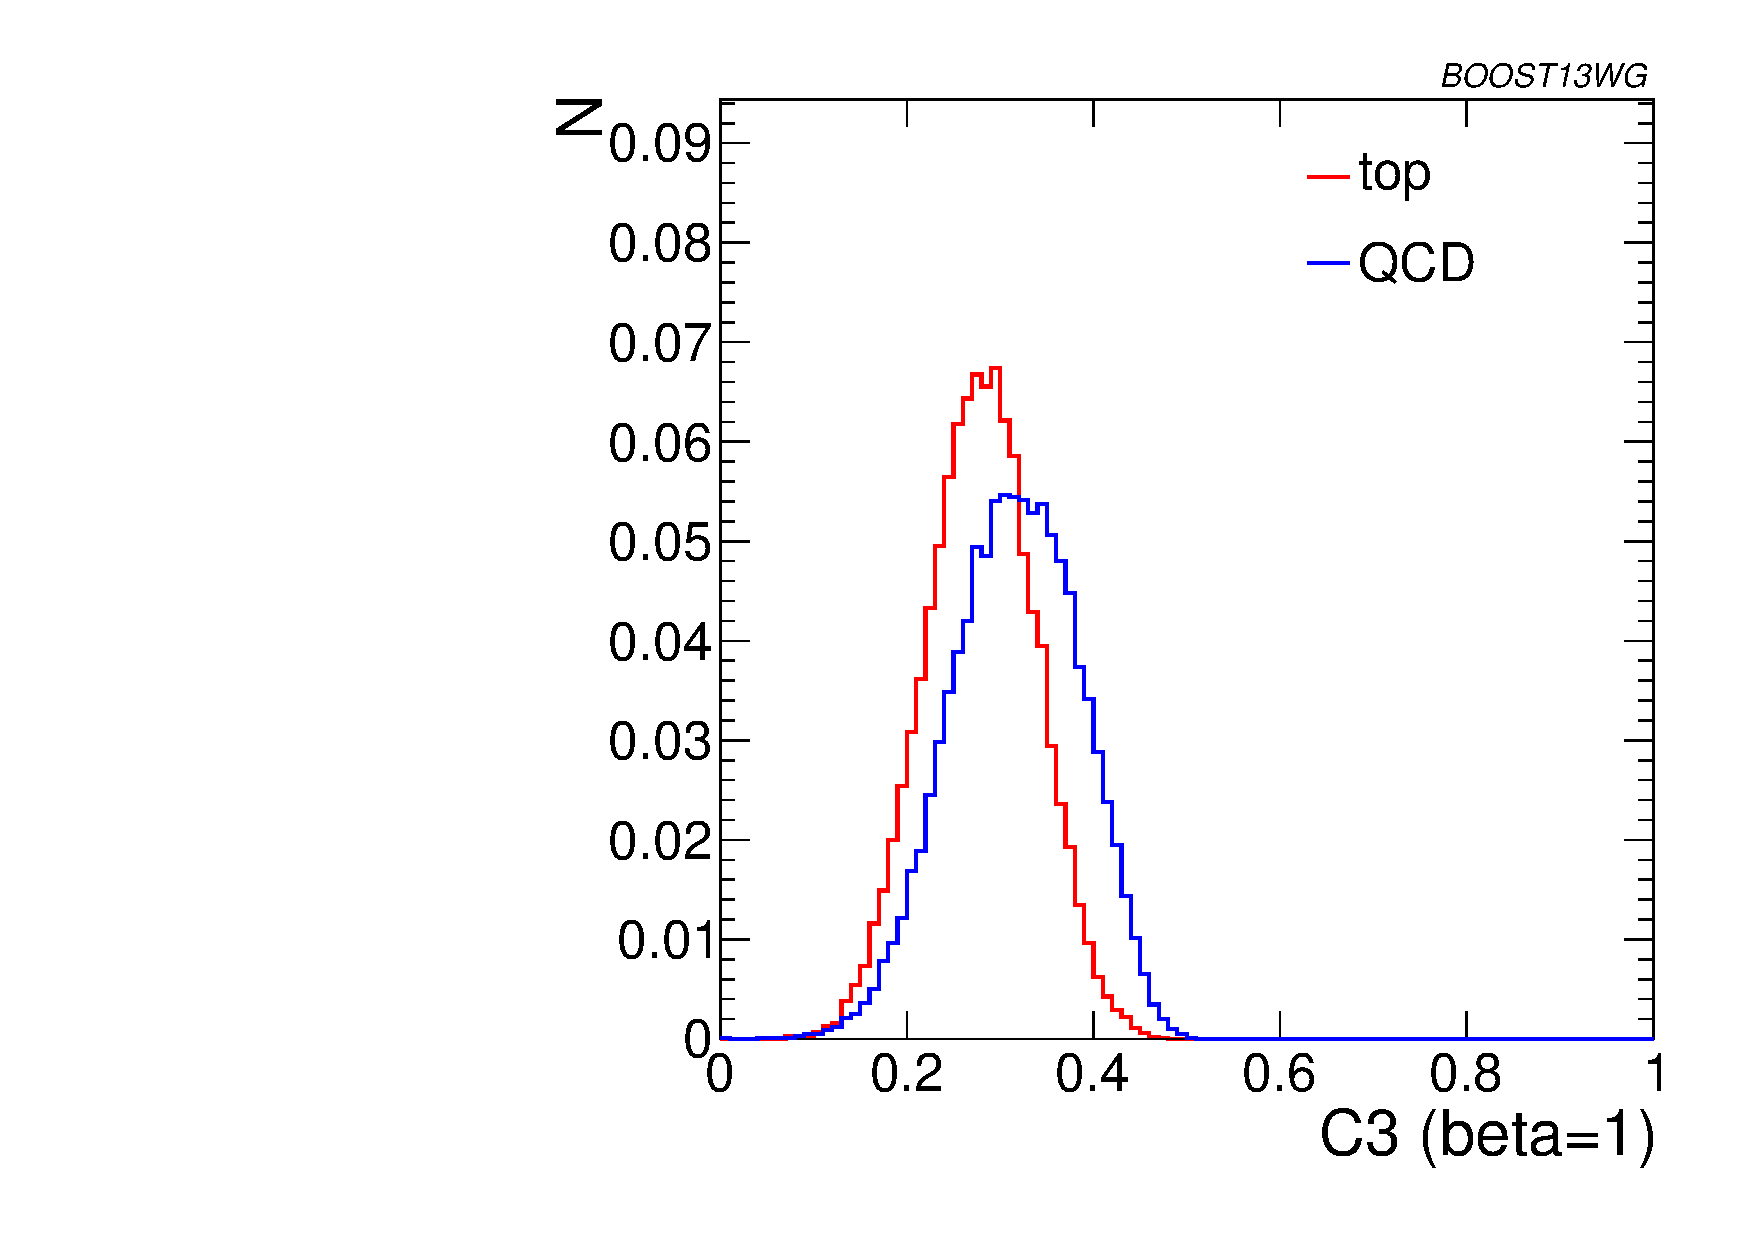
\includegraphics[width=0.32\textwidth]{./Figures/TTagging/single_variable/pT.1TeV.R.0.8/h_C3B1_pT_1_0.pdf}}
%\subfigure[$C_3^{(\beta=1)}$, $\pt=1.5-1.6$ TeV]{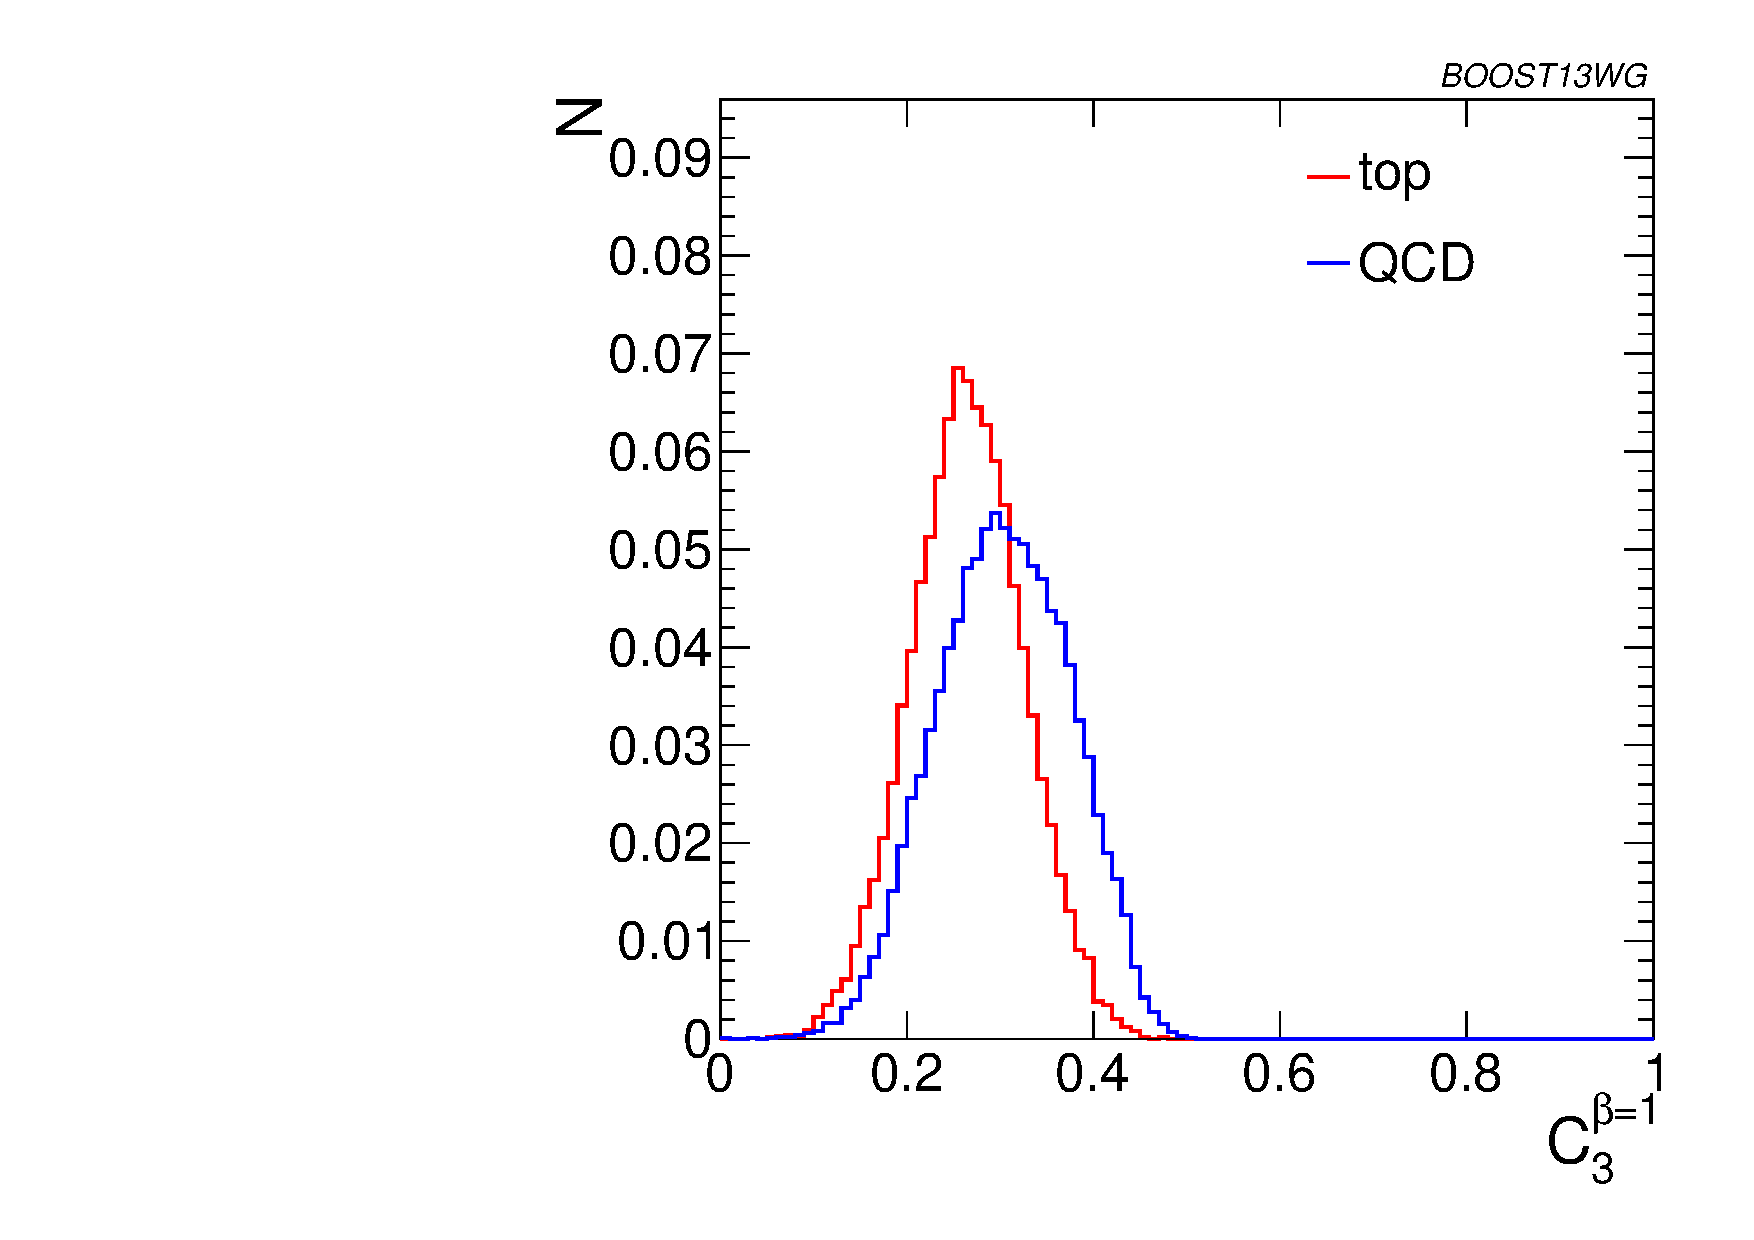
\includegraphics[width=0.32\textwidth]{./Figures/TTagging/single_variable/pT.1.5TeV.R.0.8/h_C3B1_R_0_8.pdf}}
%\caption{Comparison of $C_2^{\beta=1}$ and $C_3^{\beta=1}$ at $R=0.8$ and different values of $\pt$.}
%\label{fig:C_comparison_pT}
%
%\end{figure*}

\begin{figure*}
\centering
\subfigure[$\Gamma_{\rm Qjet}$, $\pt=600-700$ GeV]{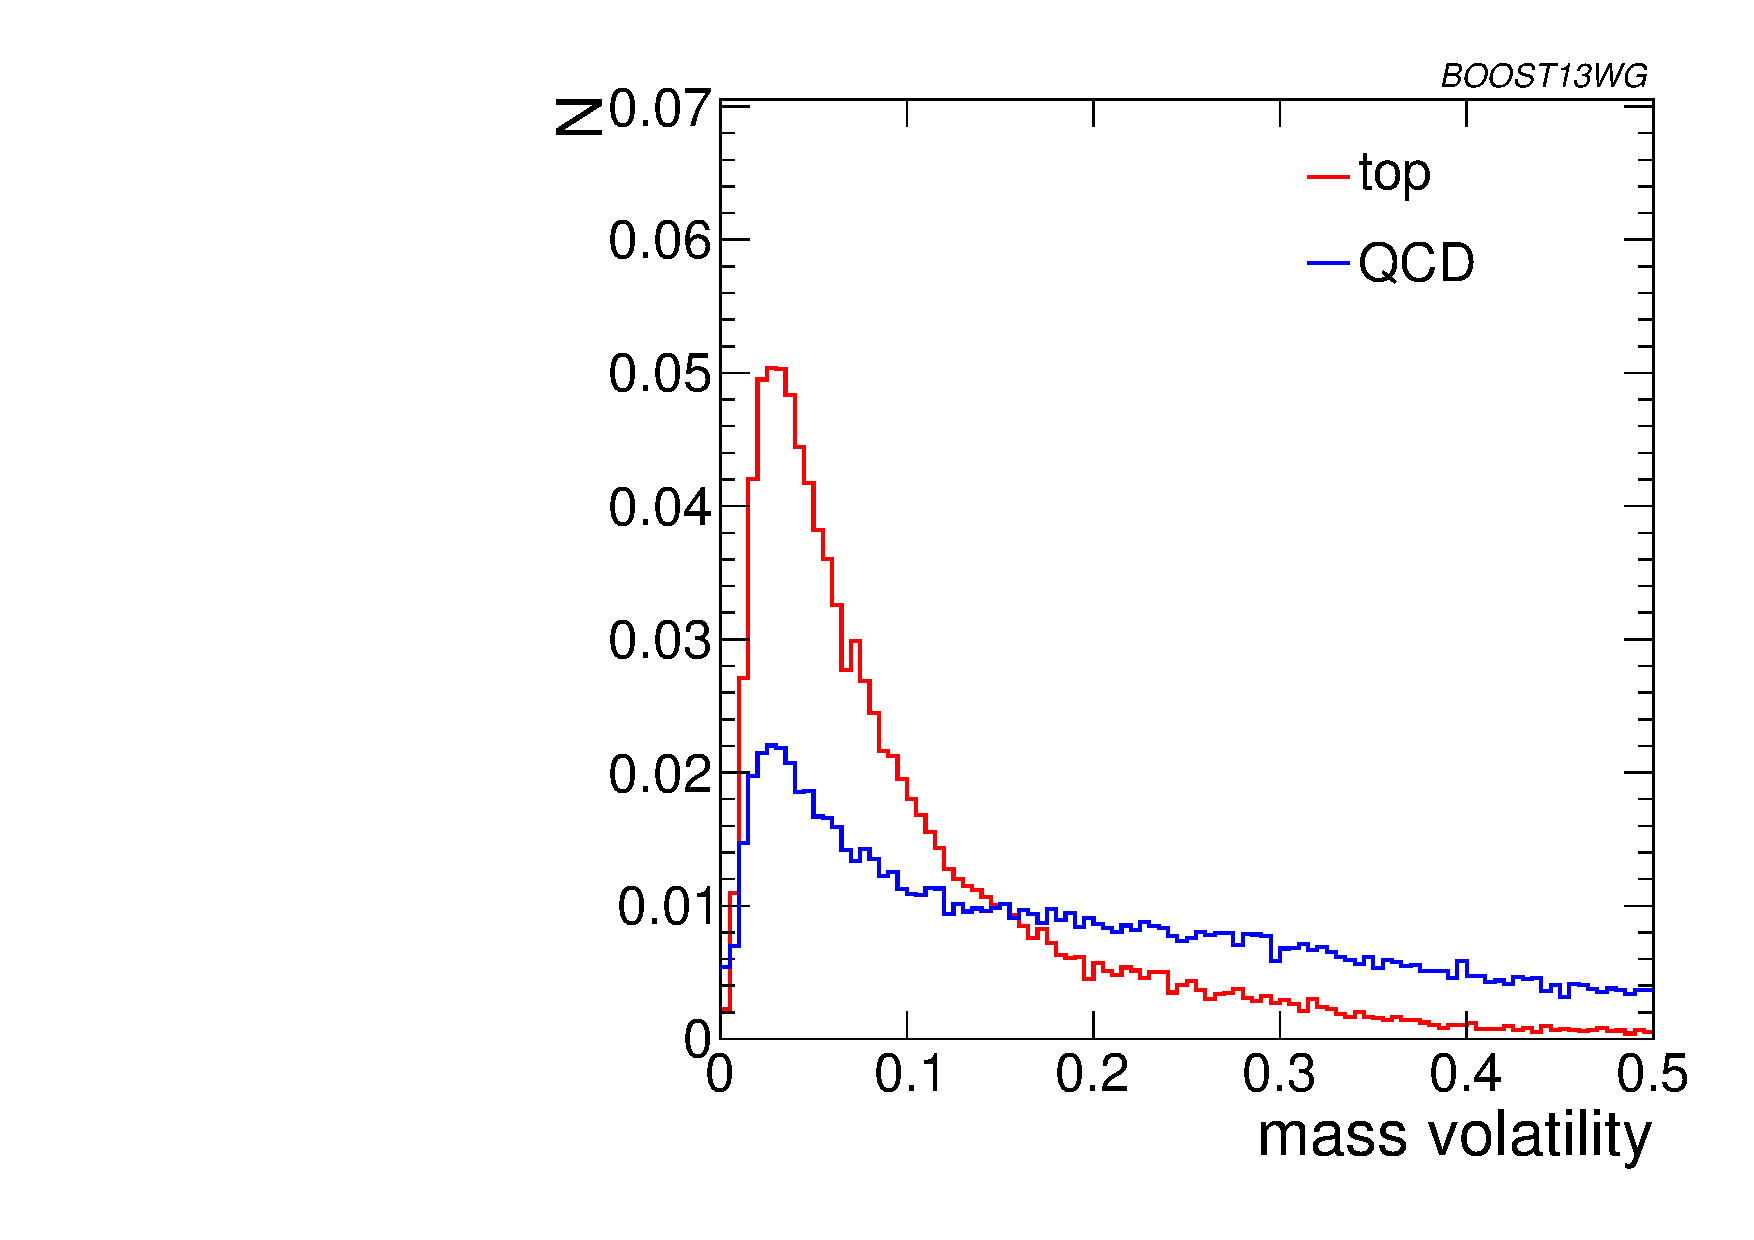
\includegraphics[width=0.245\textwidth]{./Figures/TTagging/single_variable/pT.600GeV.R.0.8/h_qjetVol_pT_0_6.pdf}}
\subfigure[$\Gamma_{\rm Qjet}$, $\pt=1.5-1.6$ TeV]{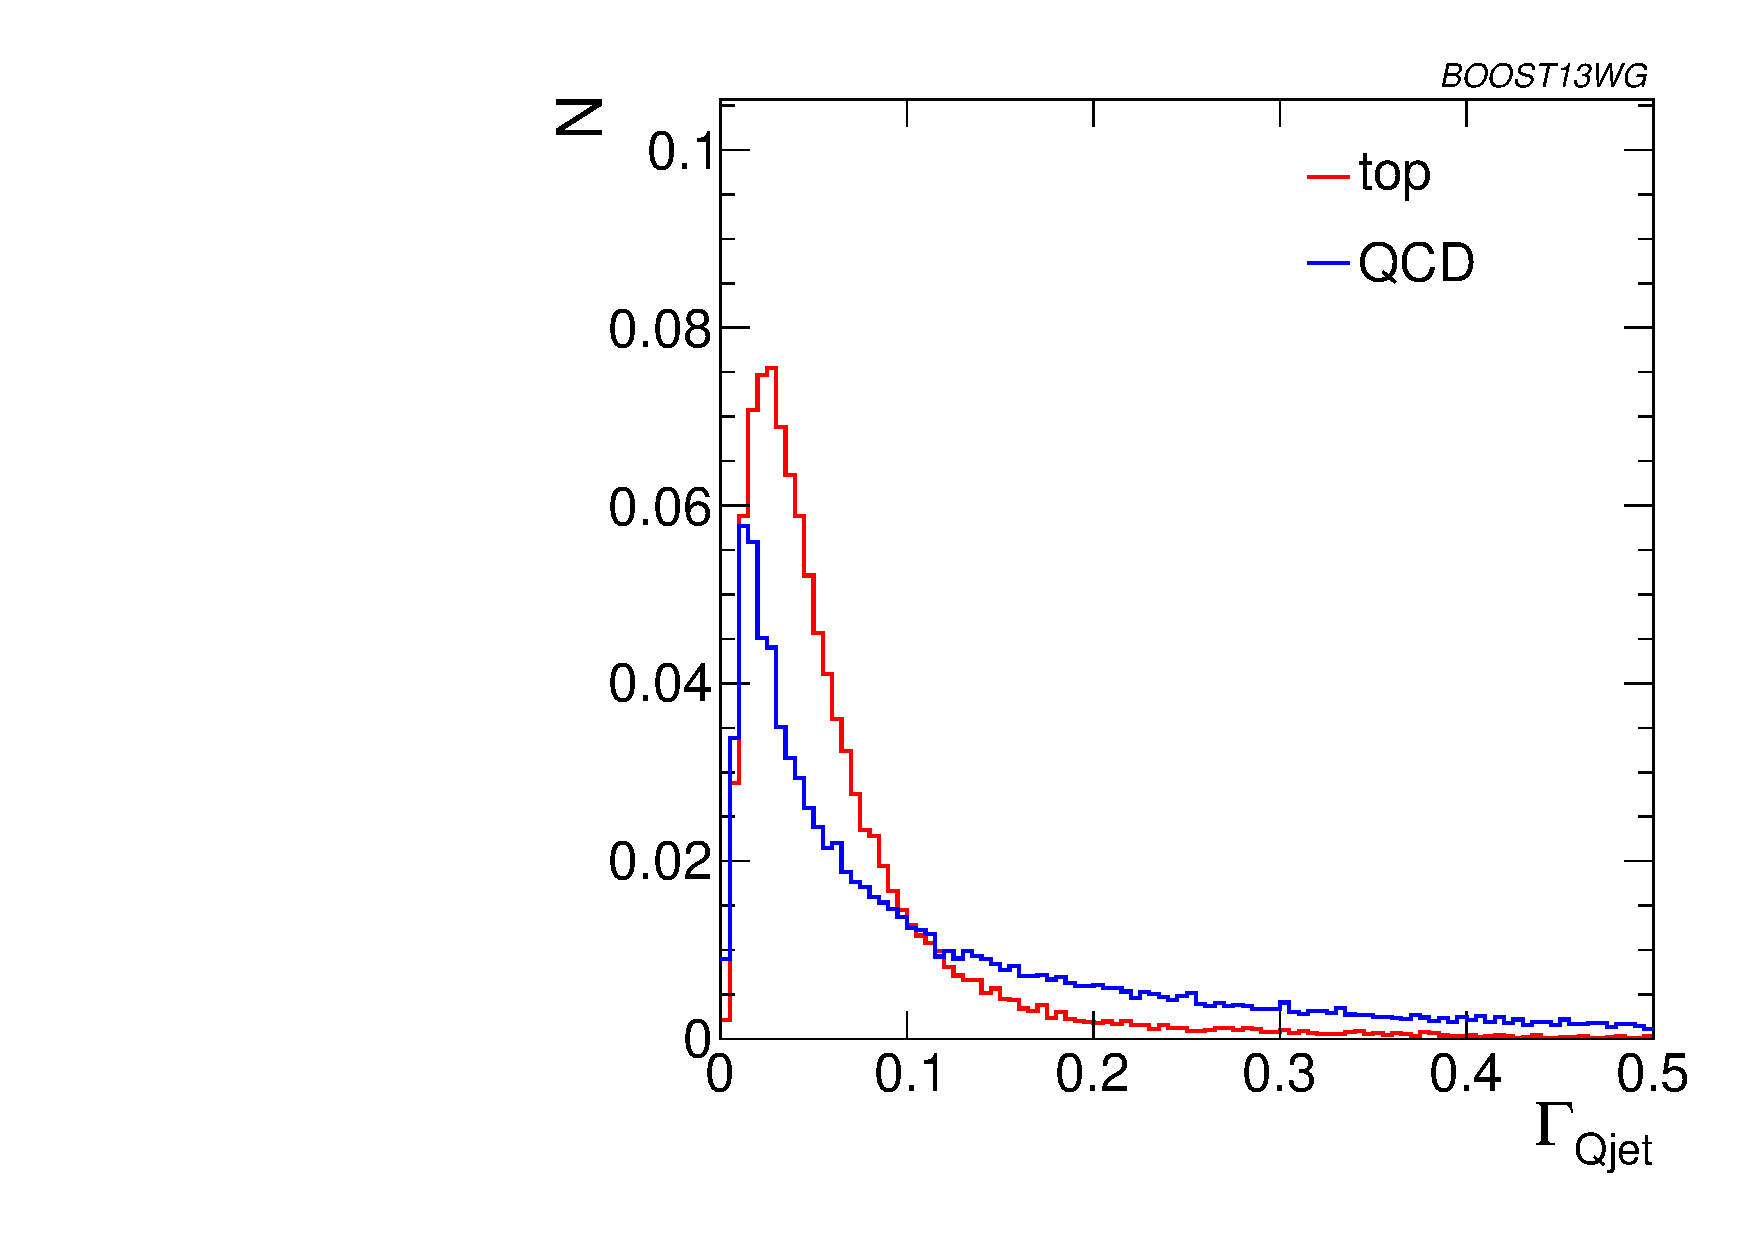
\includegraphics[width=0.245\textwidth]{./Figures/TTagging/single_variable/pT.1.5TeV.R.0.8/h_qjetVol_R_0_8.pdf}}
\subfigure[$\tau_{32}^{(\beta=1)}$, $\pt=600-700$ GeV]{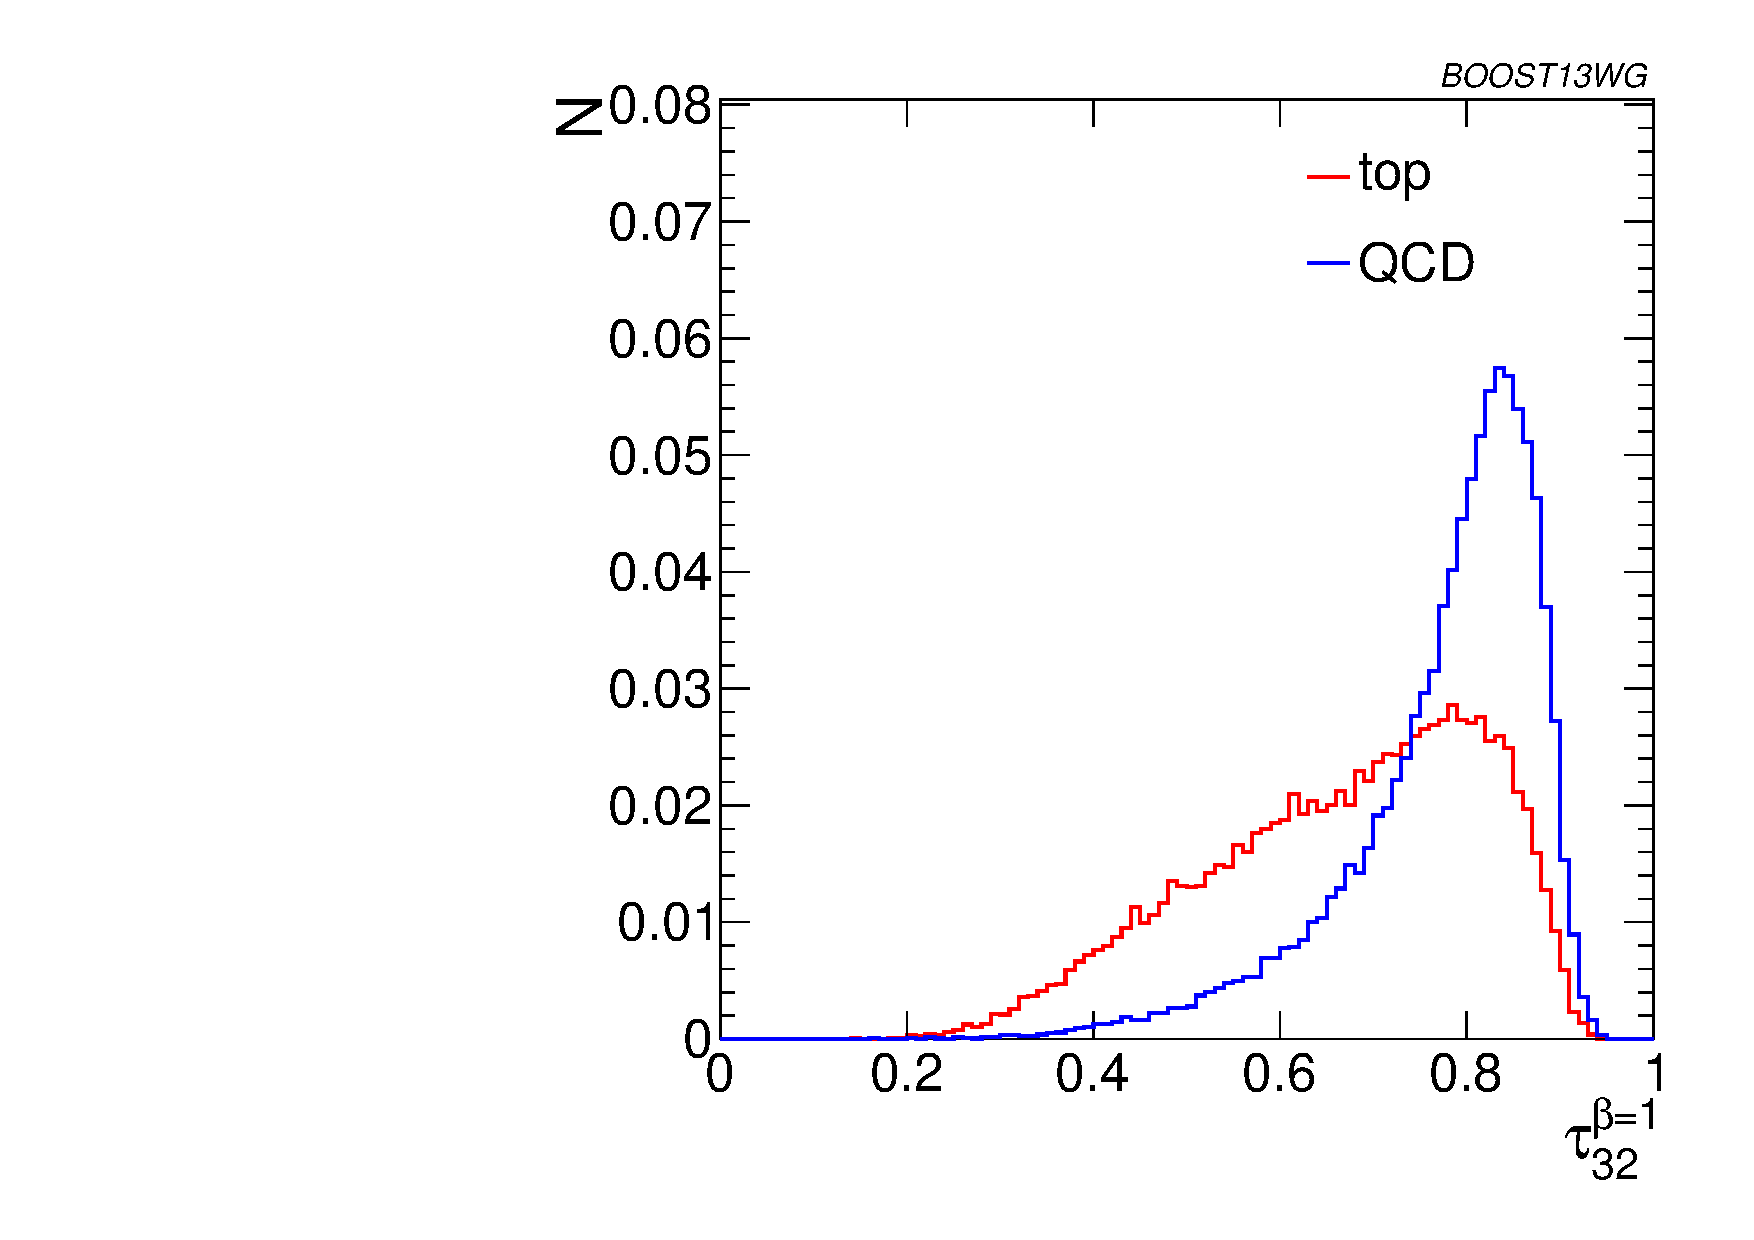
\includegraphics[width=0.245\textwidth]{./Figures/TTagging/single_variable/pT.600GeV.R.0.8/h_tau32b1_pT_0_6.pdf}}
\subfigure[$\tau_{32}^{(\beta=1)}$, $\pt=1.5-1.6$ TeV]{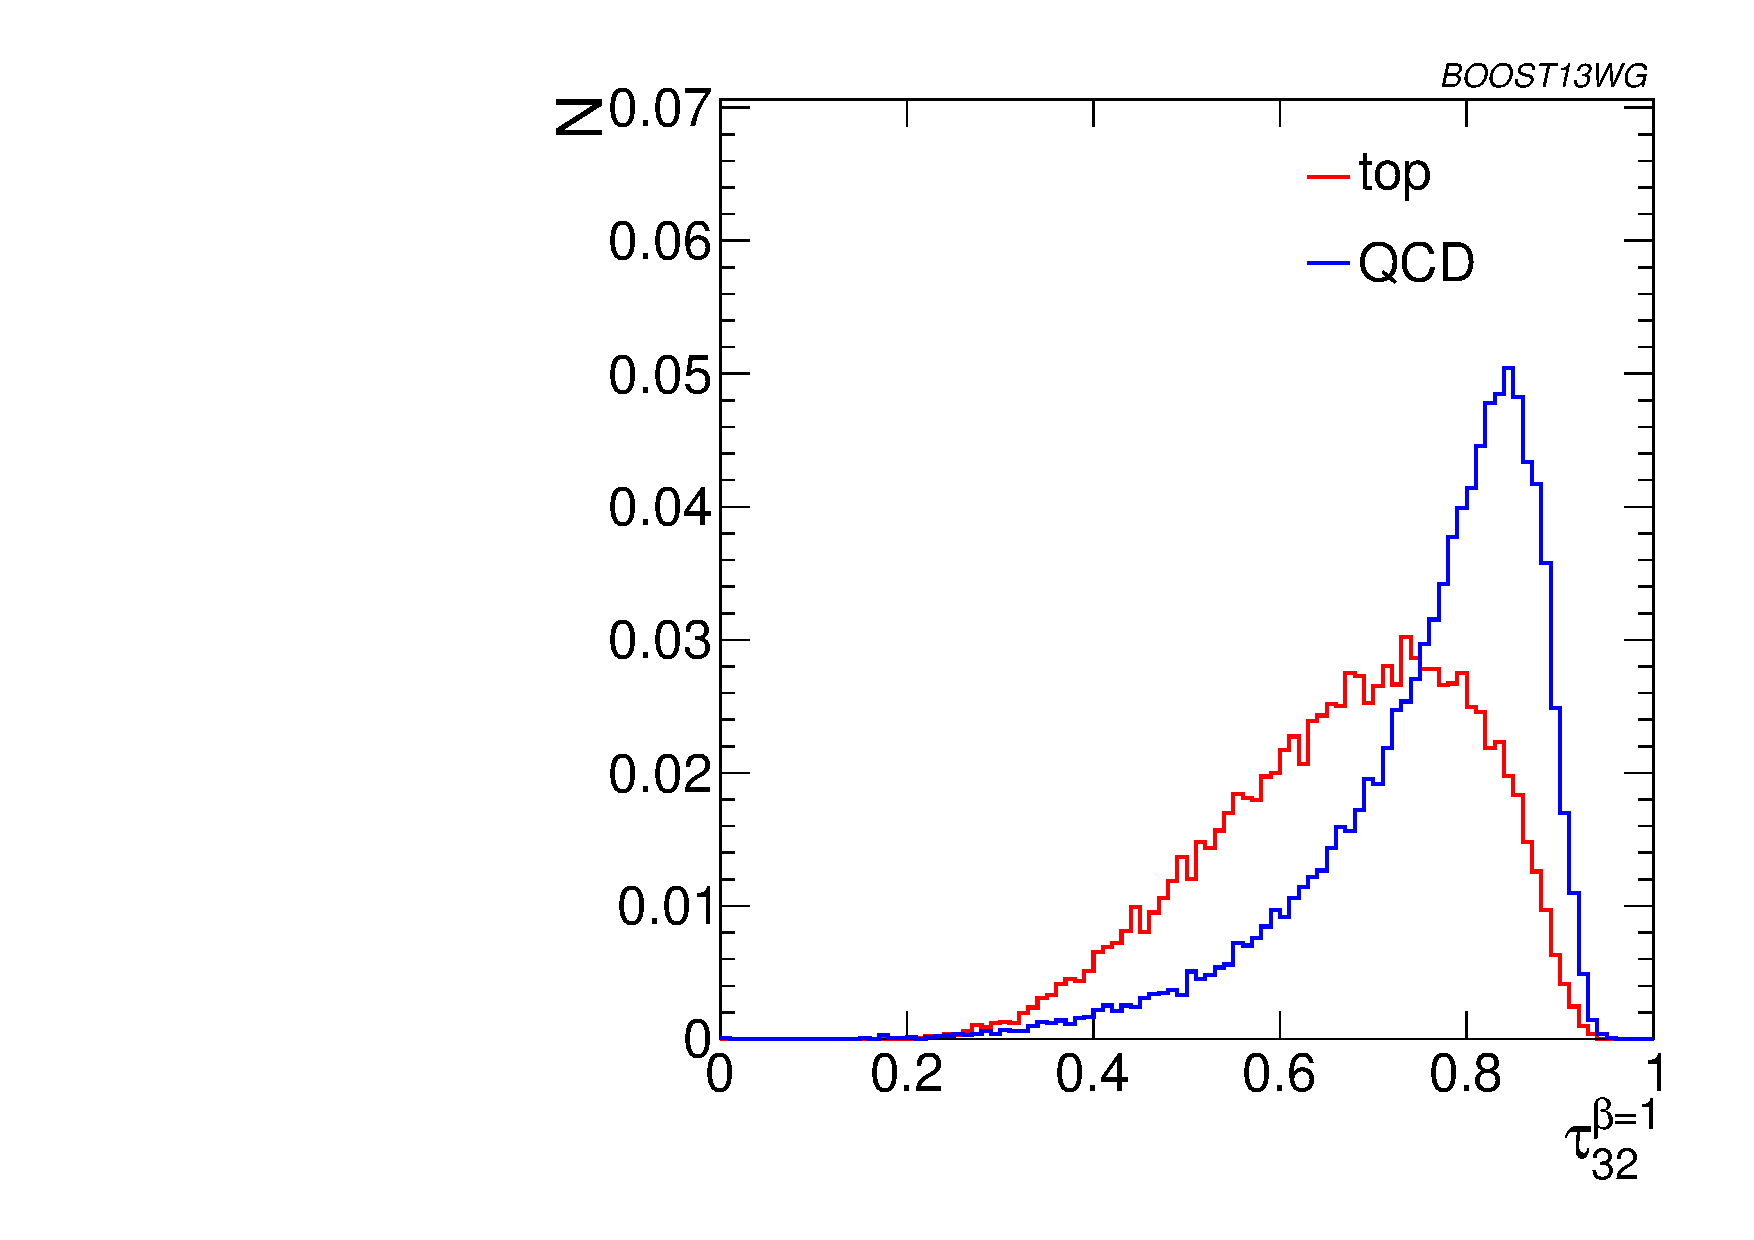
\includegraphics[width=0.245\textwidth]{./Figures/TTagging/single_variable/pT.1.5TeV.R.0.8/h_tau32b1_R_0_8.pdf}}
\caption{Comparison of $\Gamma_{\rm Qjet}$ and $\tau_{32}^{\beta=1}$ at $R=0.8$ and different values of the $\pt$. These shape observables are the most sensitive to varying $\pt$.}
\label{fig:Qjet_comparison_pT}
\end{figure*}

%\begin{figure*}
%\centering
%\subfigure[$\Gamma_{\rm Qjet}$, $\pt=600-700$ GeV]{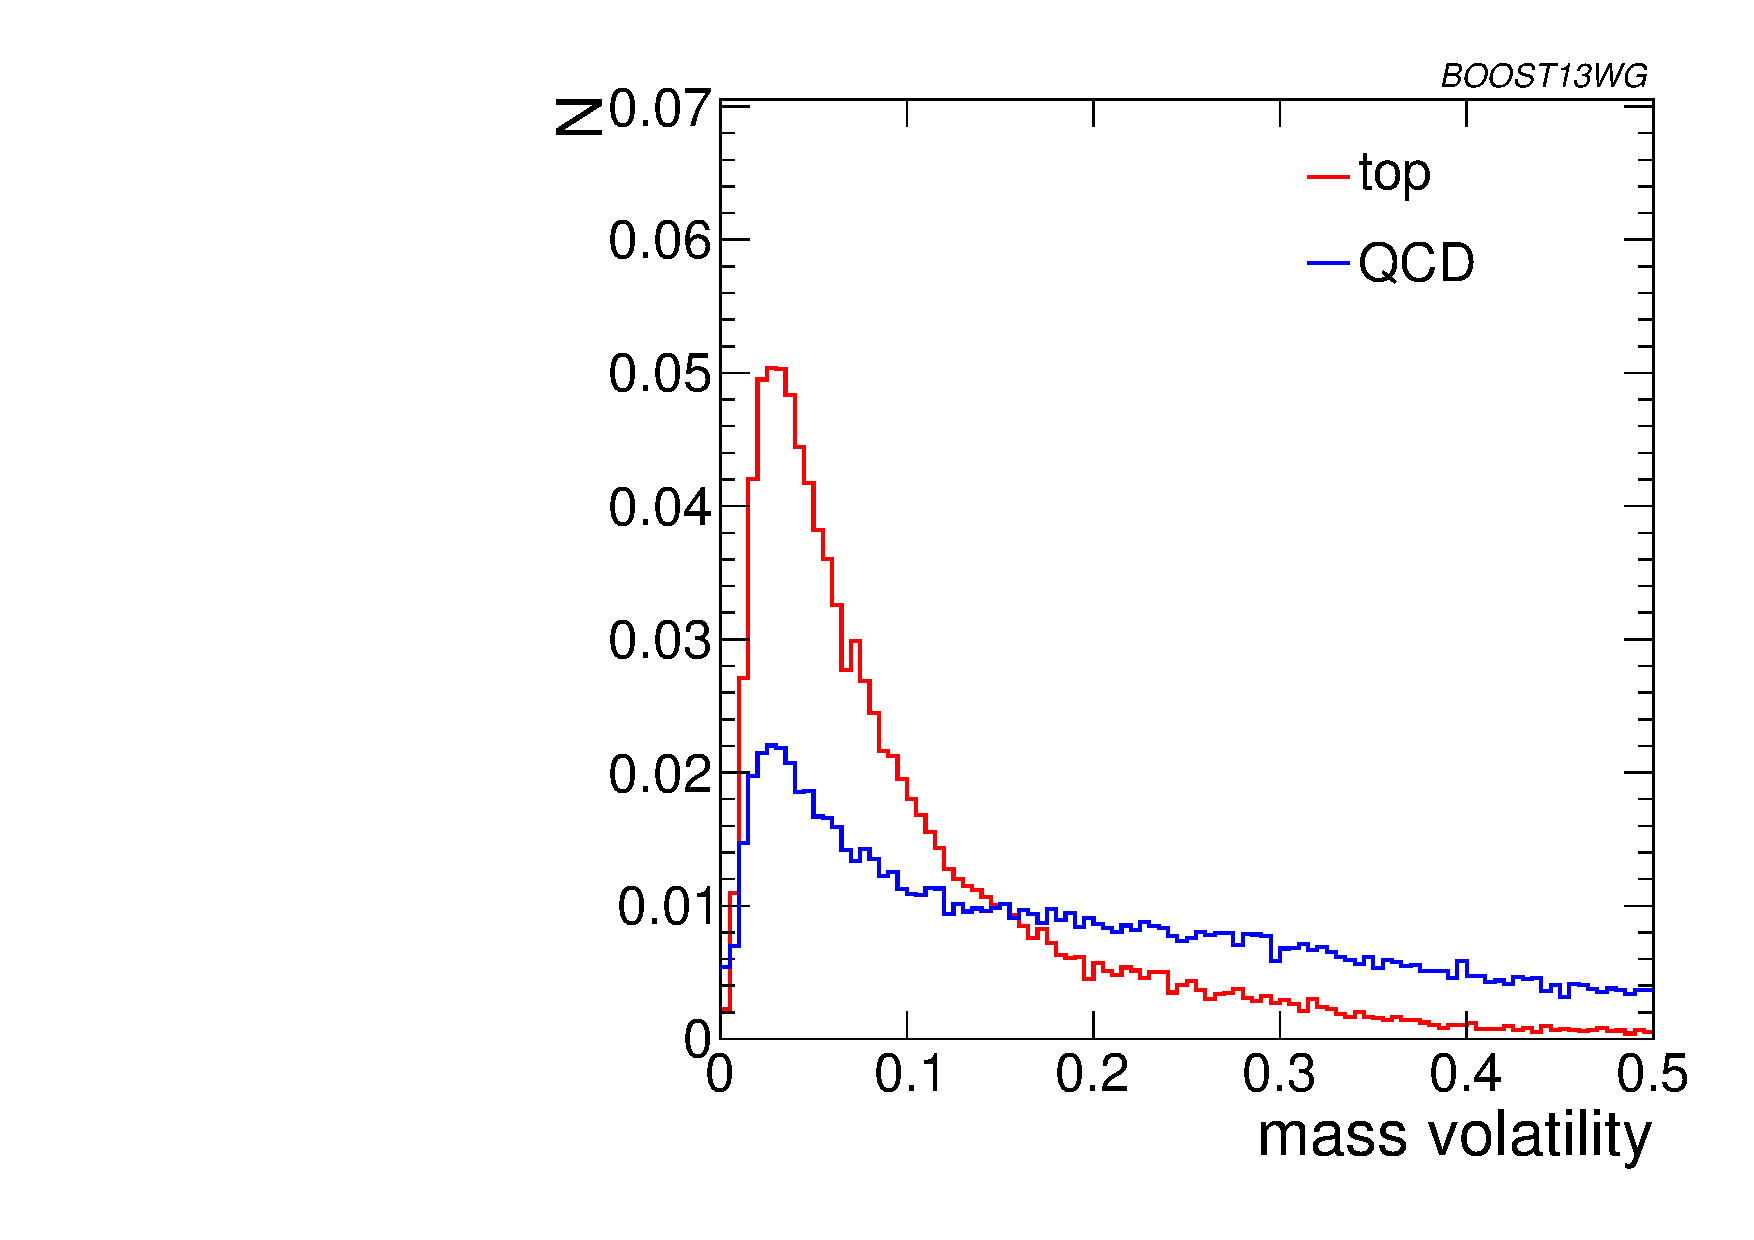
\includegraphics[width=0.32\textwidth]{./Figures/TTagging/single_variable/pT.600GeV.R.0.8/h_qjetVol_pT_0_6.pdf}}
%\subfigure[$\Gamma_{\rm Qjet}$, $\pt=1-1.1$ TeV]{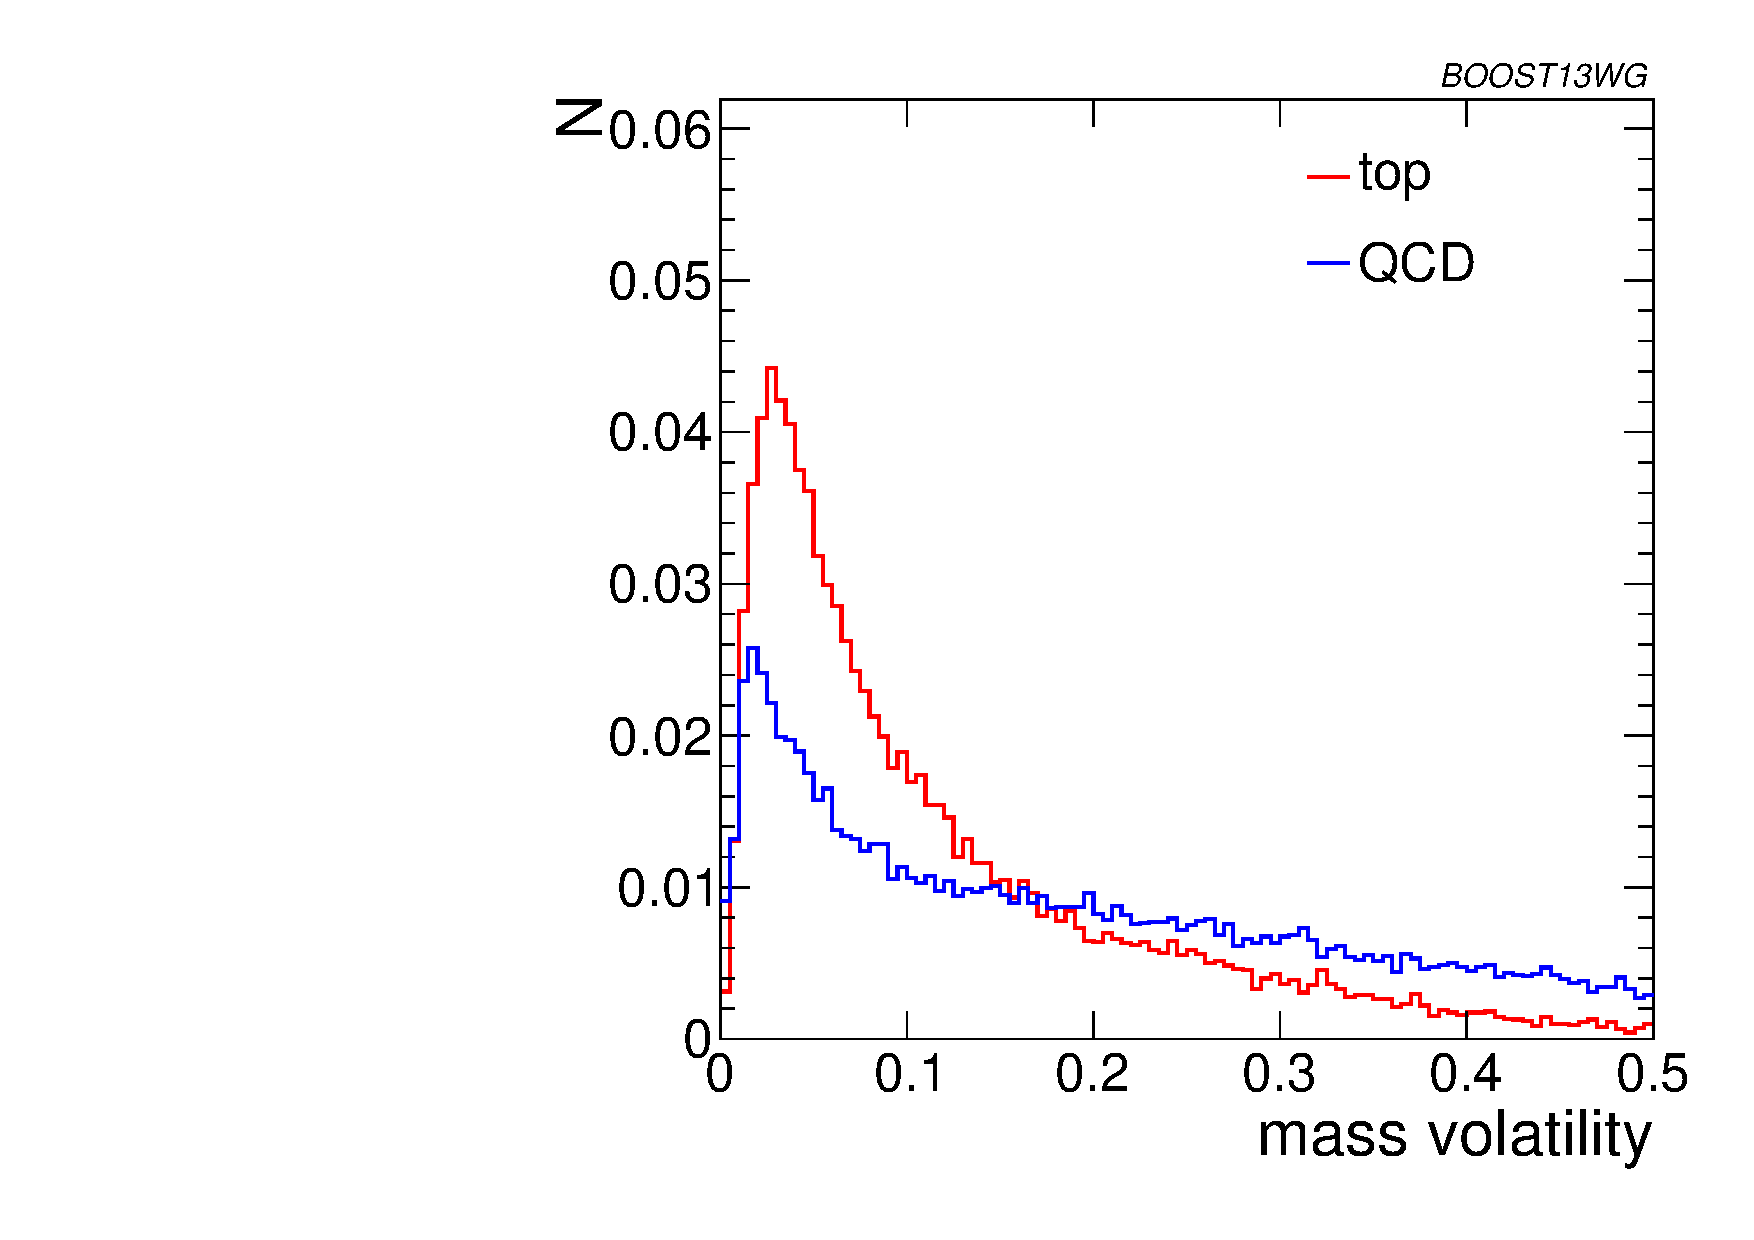
\includegraphics[width=0.32\textwidth]{./Figures/TTagging/single_variable/pT.1TeV.R.0.8/h_qjetVol_pT_1_0.pdf}}
%\subfigure[$\Gamma_{\rm Qjet}$, $\pt=1.5-1.6$ TeV]{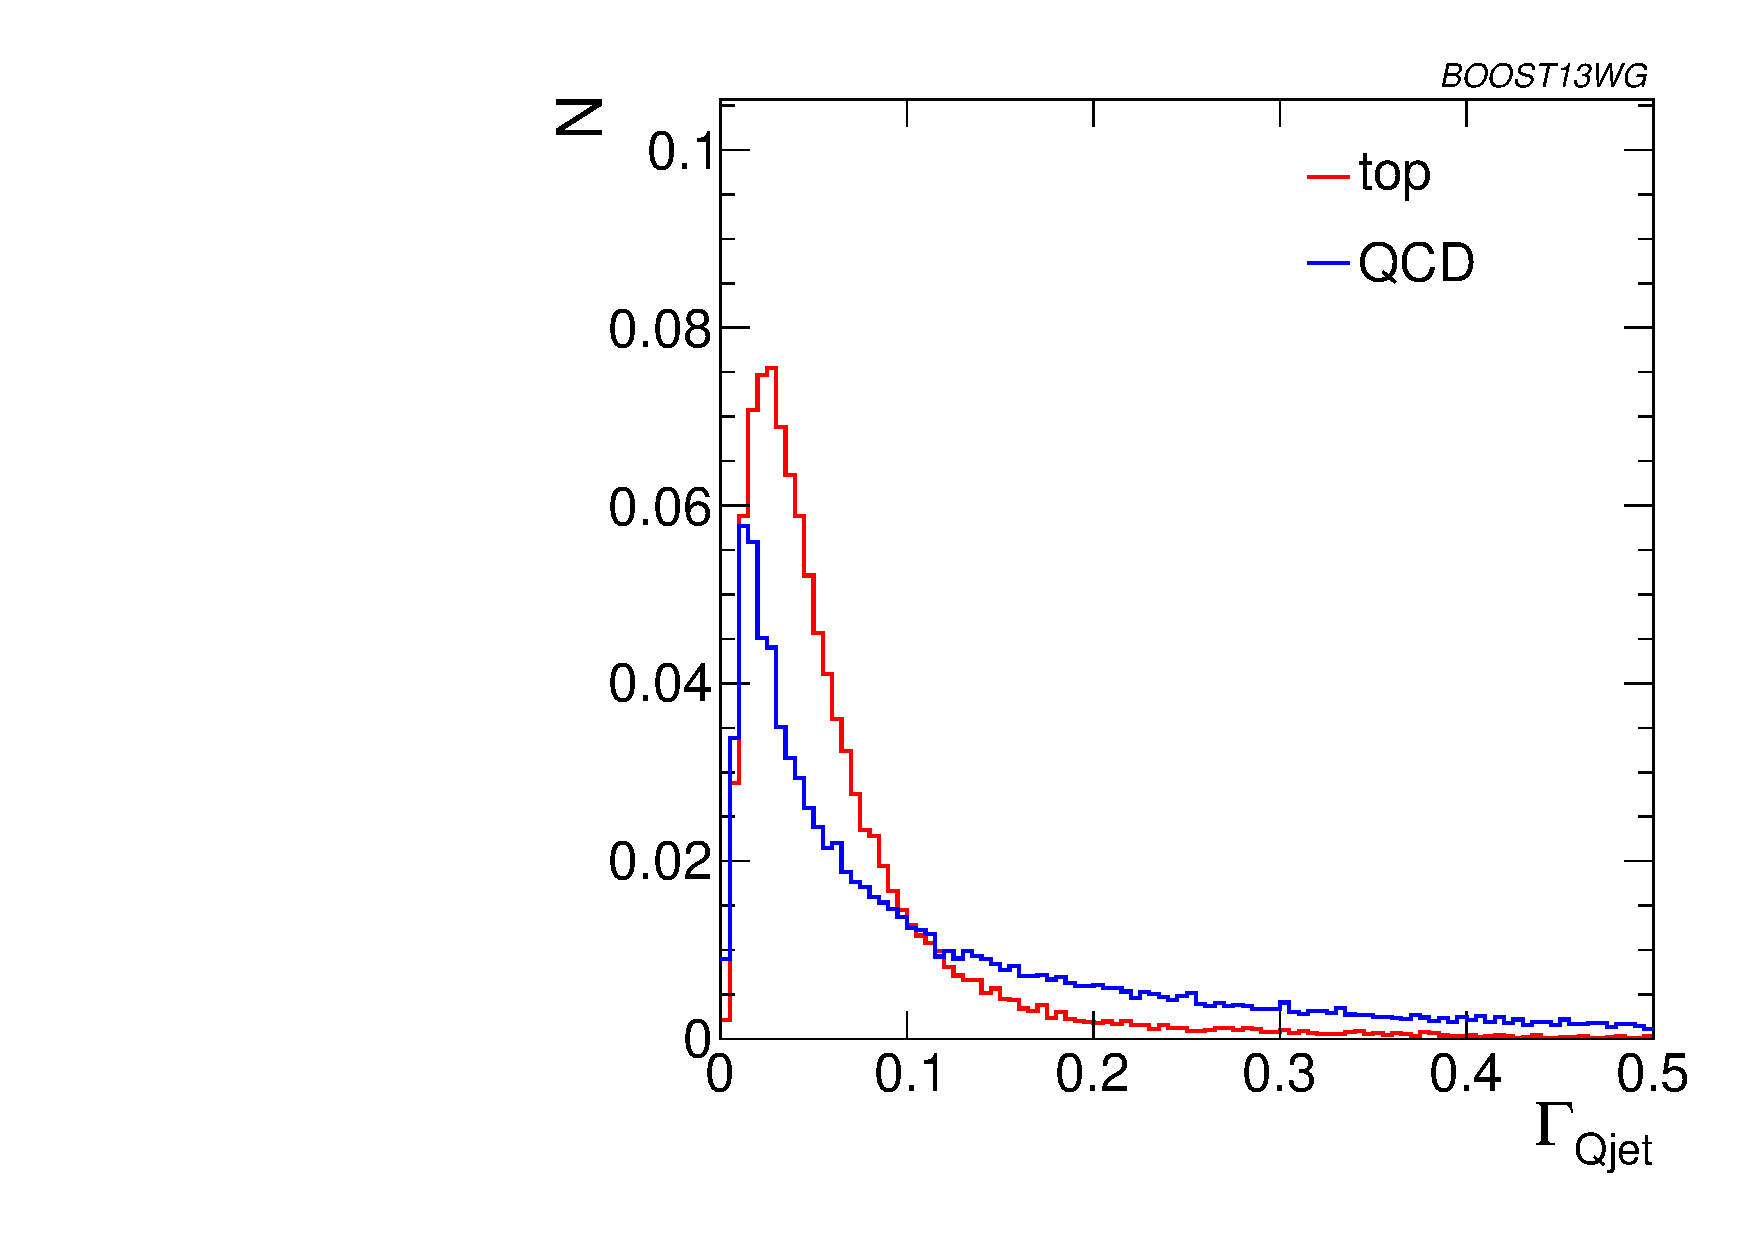
\includegraphics[width=0.32\textwidth]{./Figures/TTagging/single_variable/pT.1.5TeV.R.0.8/h_qjetVol_R_0_8.pdf}}
%\caption{Comparison of $\Gamma_{\rm Qjet}$ and $\tau_{32}^{\beta=1}$ at $R=0.8$ and different values of the $\pt$.}
%\label{fig:Qjet_comparison_pT}
%
%\end{figure*}

%\begin{figure*}
%\centering
%\subfigure[$\tau_{21}^{(\beta=1)}$, $\pt=600-700$ GeV]{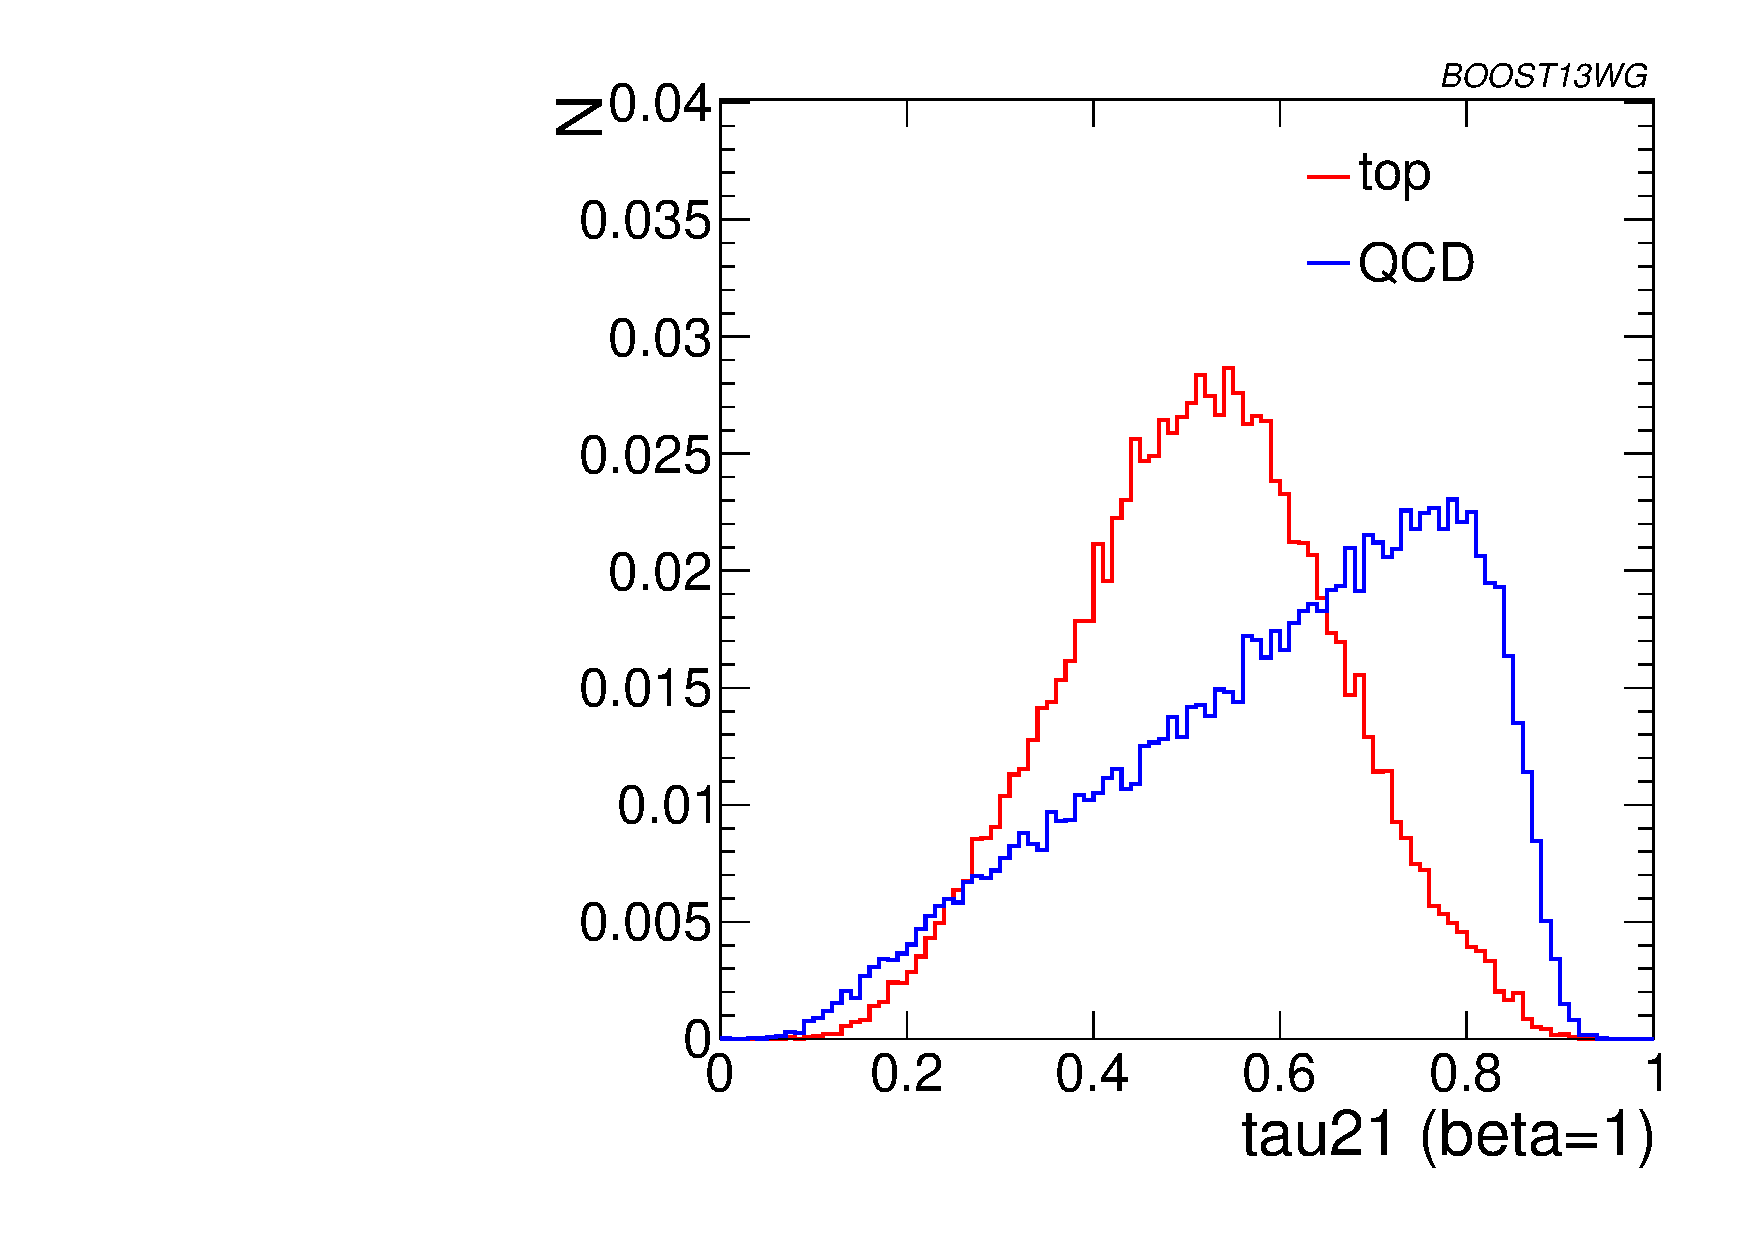
\includegraphics[width=0.32\textwidth]{./Figures/TTagging/single_variable/pT.600GeV.R.0.8/h_tau21b1_pT_0_6.pdf}}
%\subfigure[$\tau_{21}^{(\beta=1)}$, $\pt=1-1.1$ TeV]{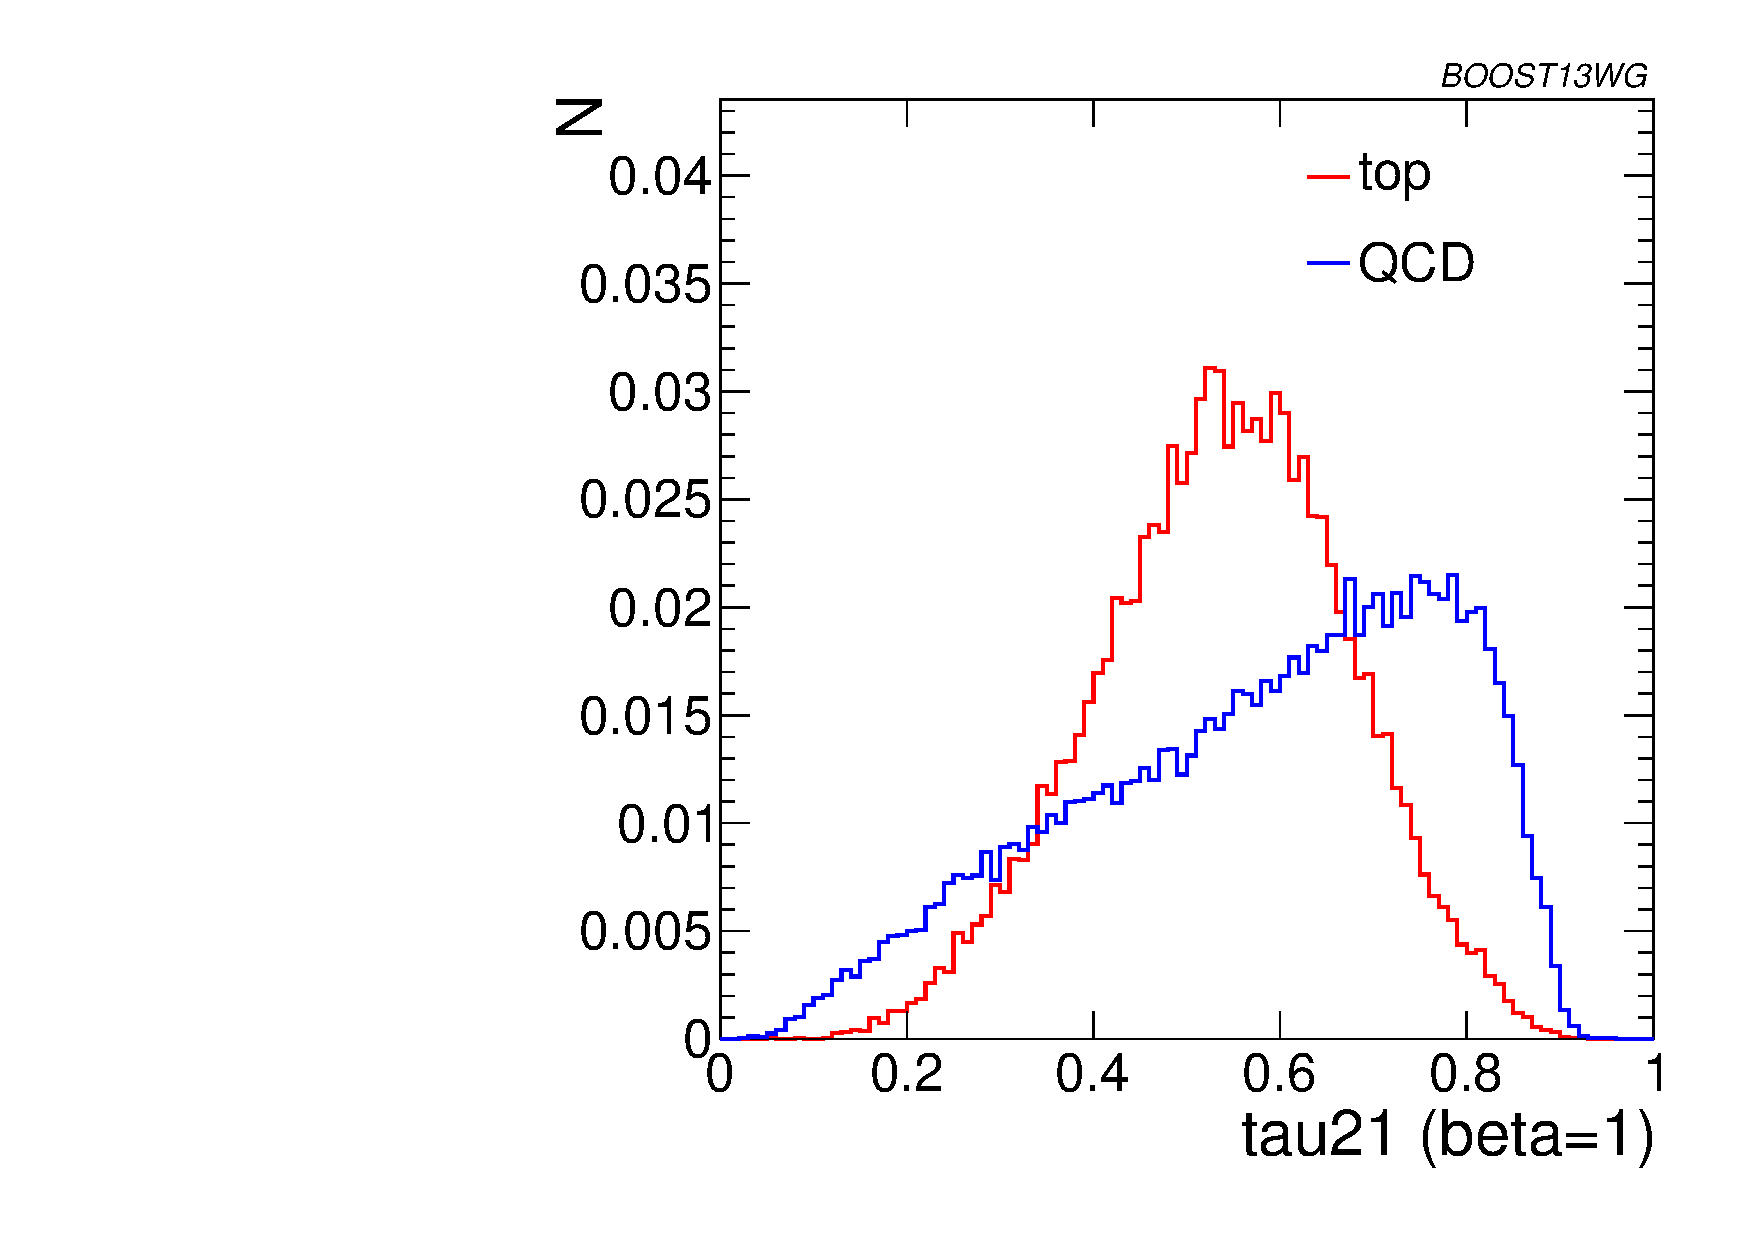
\includegraphics[width=0.32\textwidth]{./Figures/TTagging/single_variable/pT.1TeV.R.0.8/h_tau21b1_pT_1_0.pdf}}
%\subfigure[$\tau_{21}^{(\beta=1)}$, $\pt=1.5-1.6$ TeV]{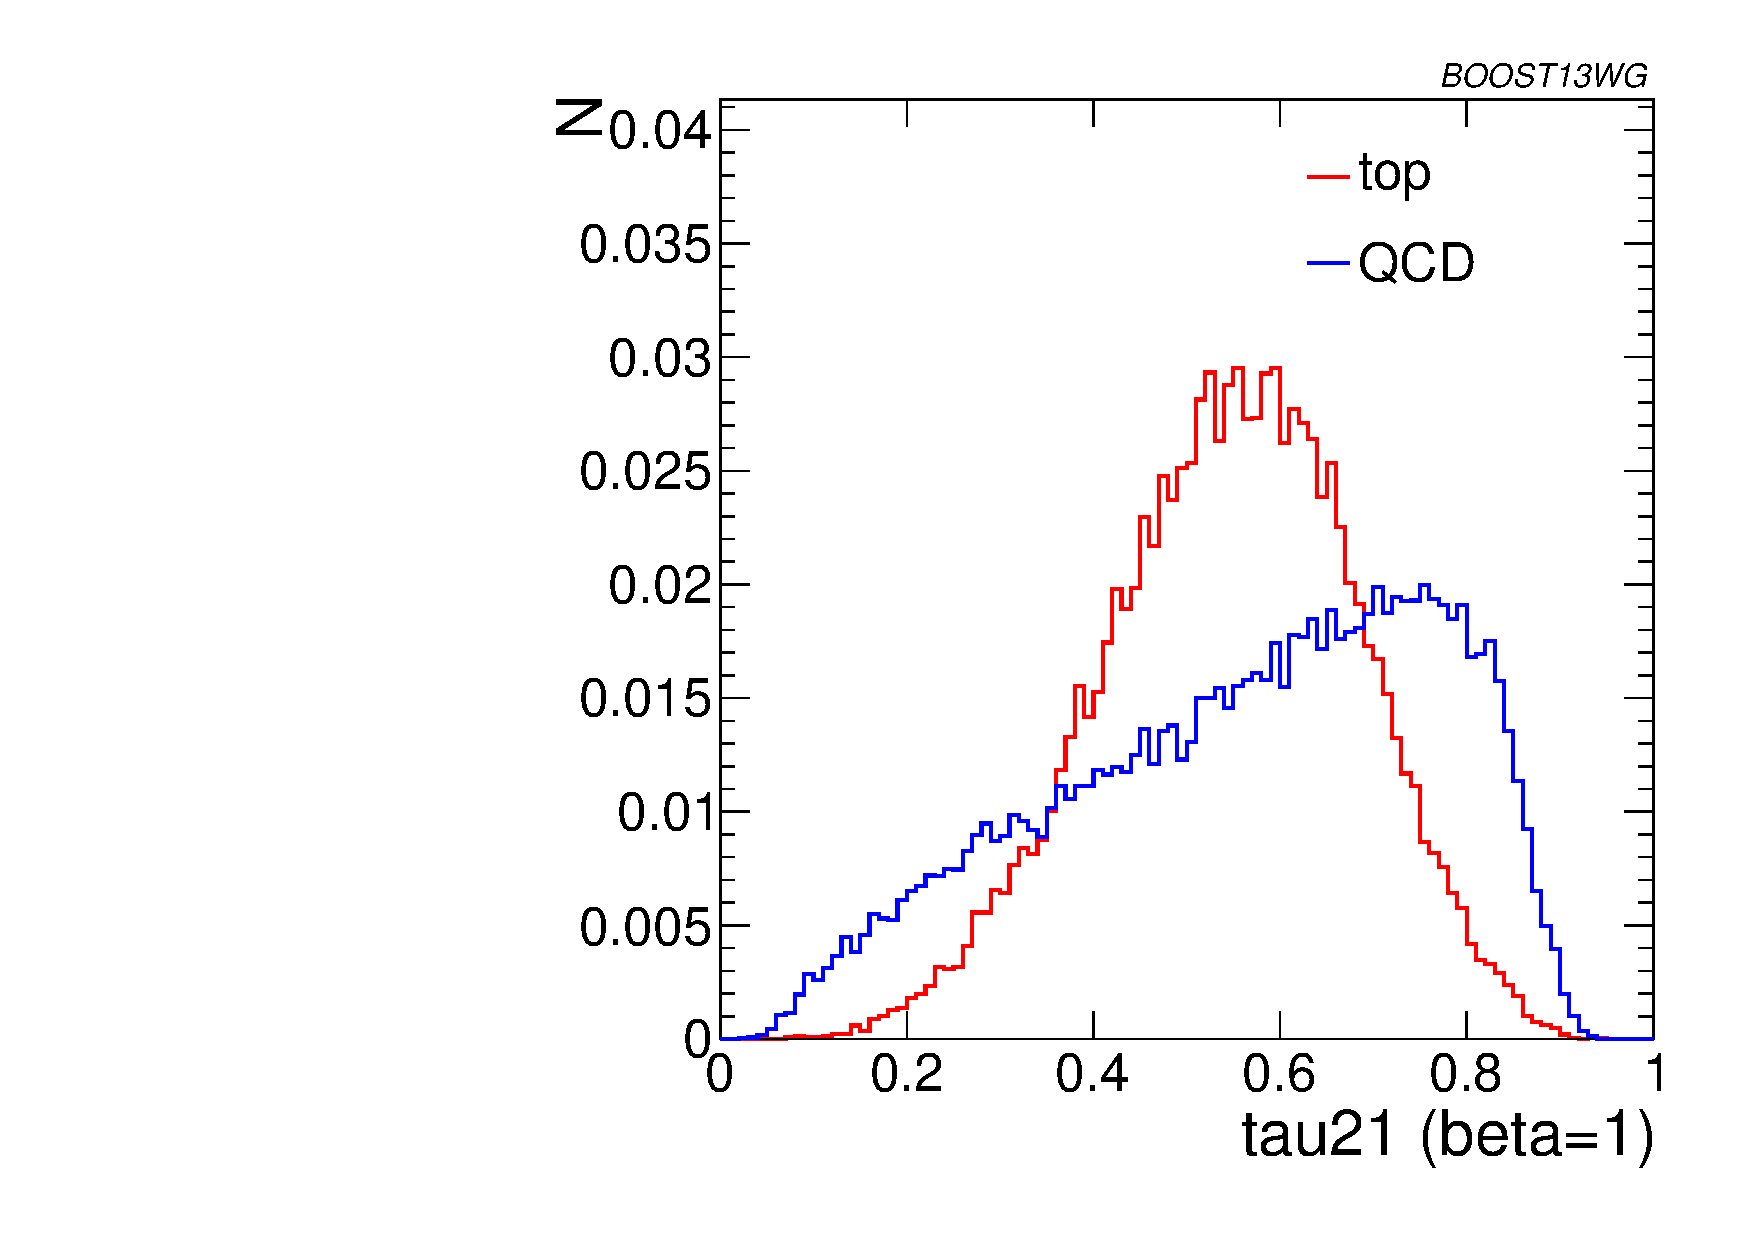
\includegraphics[width=0.32\textwidth]{./Figures/TTagging/single_variable/pT.1.5TeV.R.0.8/h_tau21b1_R_0_8.pdf}}
%\subfigure[$\tau_{32}^{(\beta=1)}$, $\pt=600-700$ GeV]{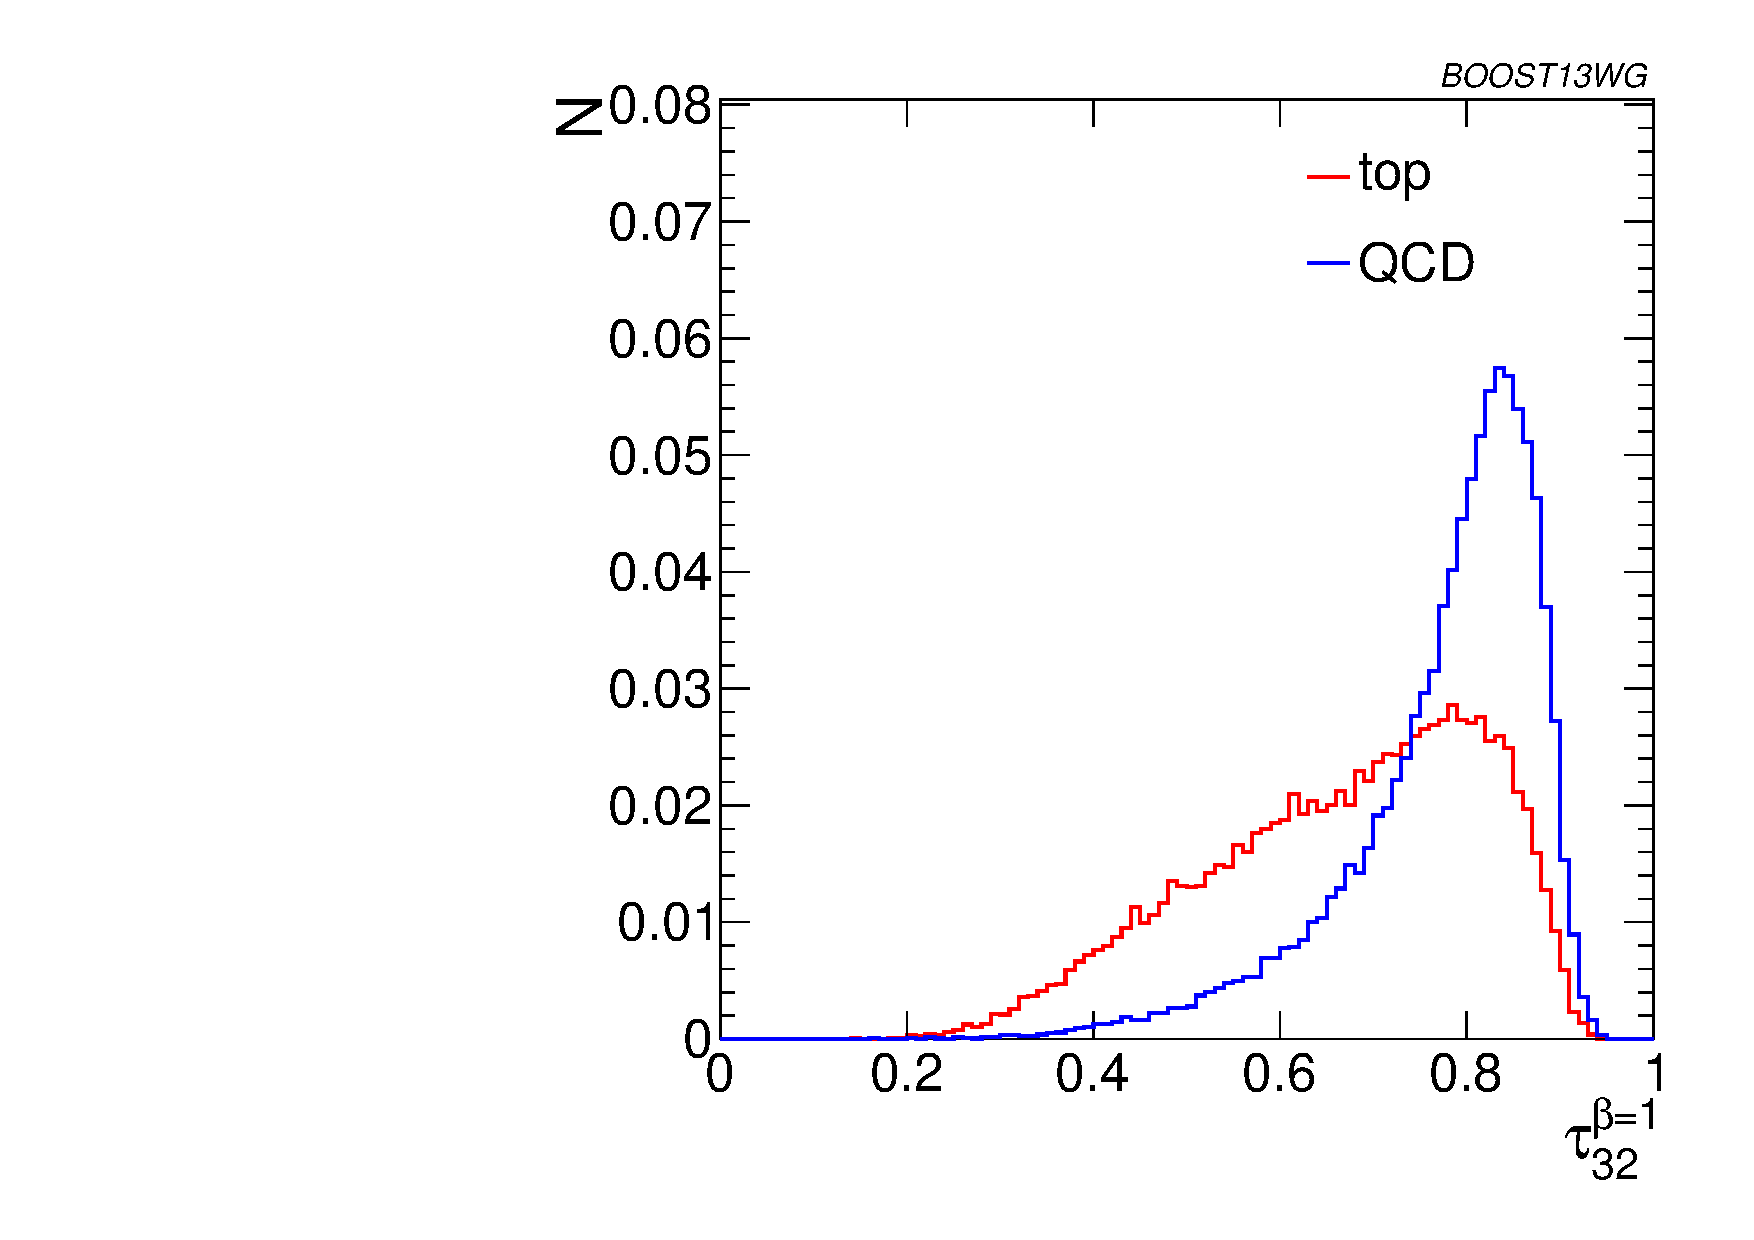
\includegraphics[width=0.32\textwidth]{./Figures/TTagging/single_variable/pT.600GeV.R.0.8/h_tau32b1_pT_0_6.pdf}}
%\subfigure[$\tau_{32}^{(\beta=1)}$, $\pt=1-1.1$ TeV]{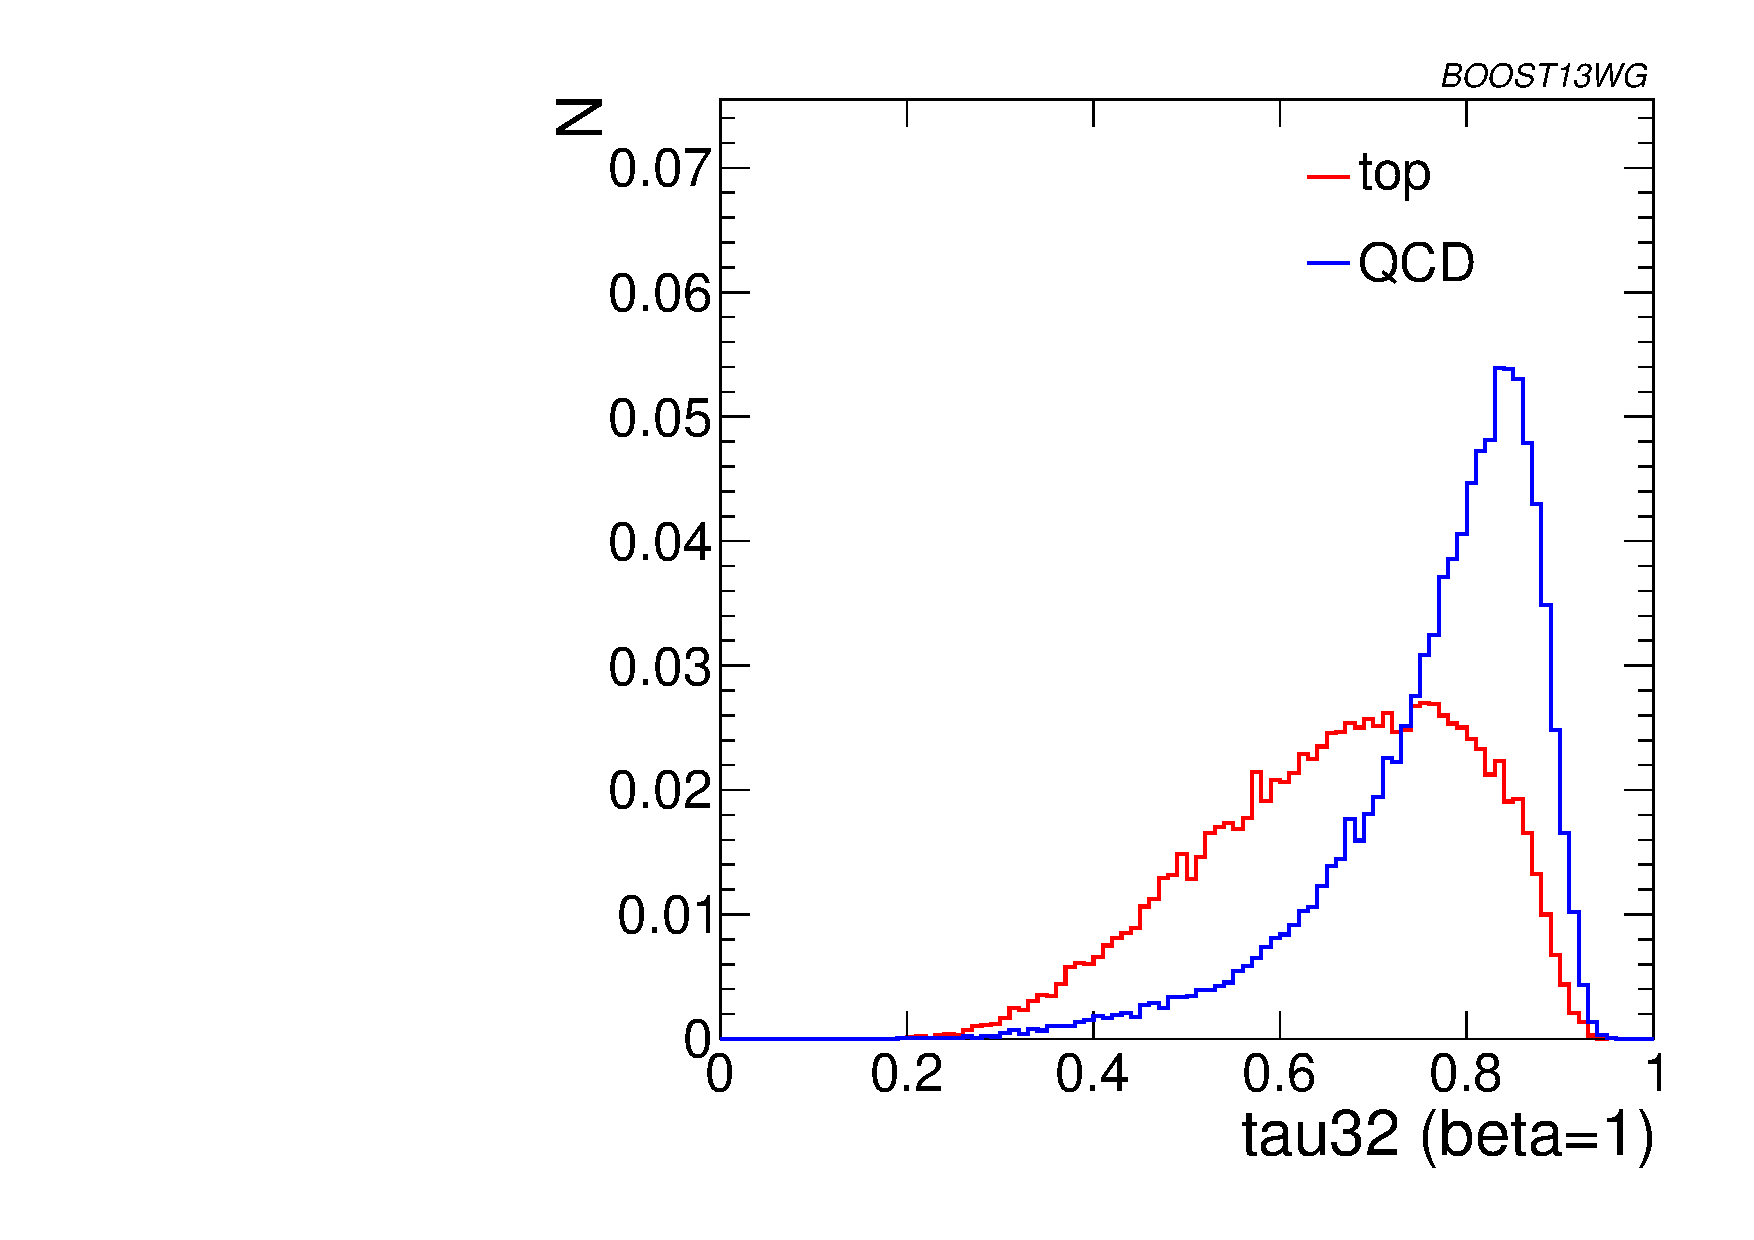
\includegraphics[width=0.32\textwidth]{./Figures/TTagging/single_variable/pT.1TeV.R.0.8/h_tau32b1_pT_1_0.pdf}}
%\subfigure[$\tau_{32}^{(\beta=1)}$, $\pt=1.5-1.6$ TeV]{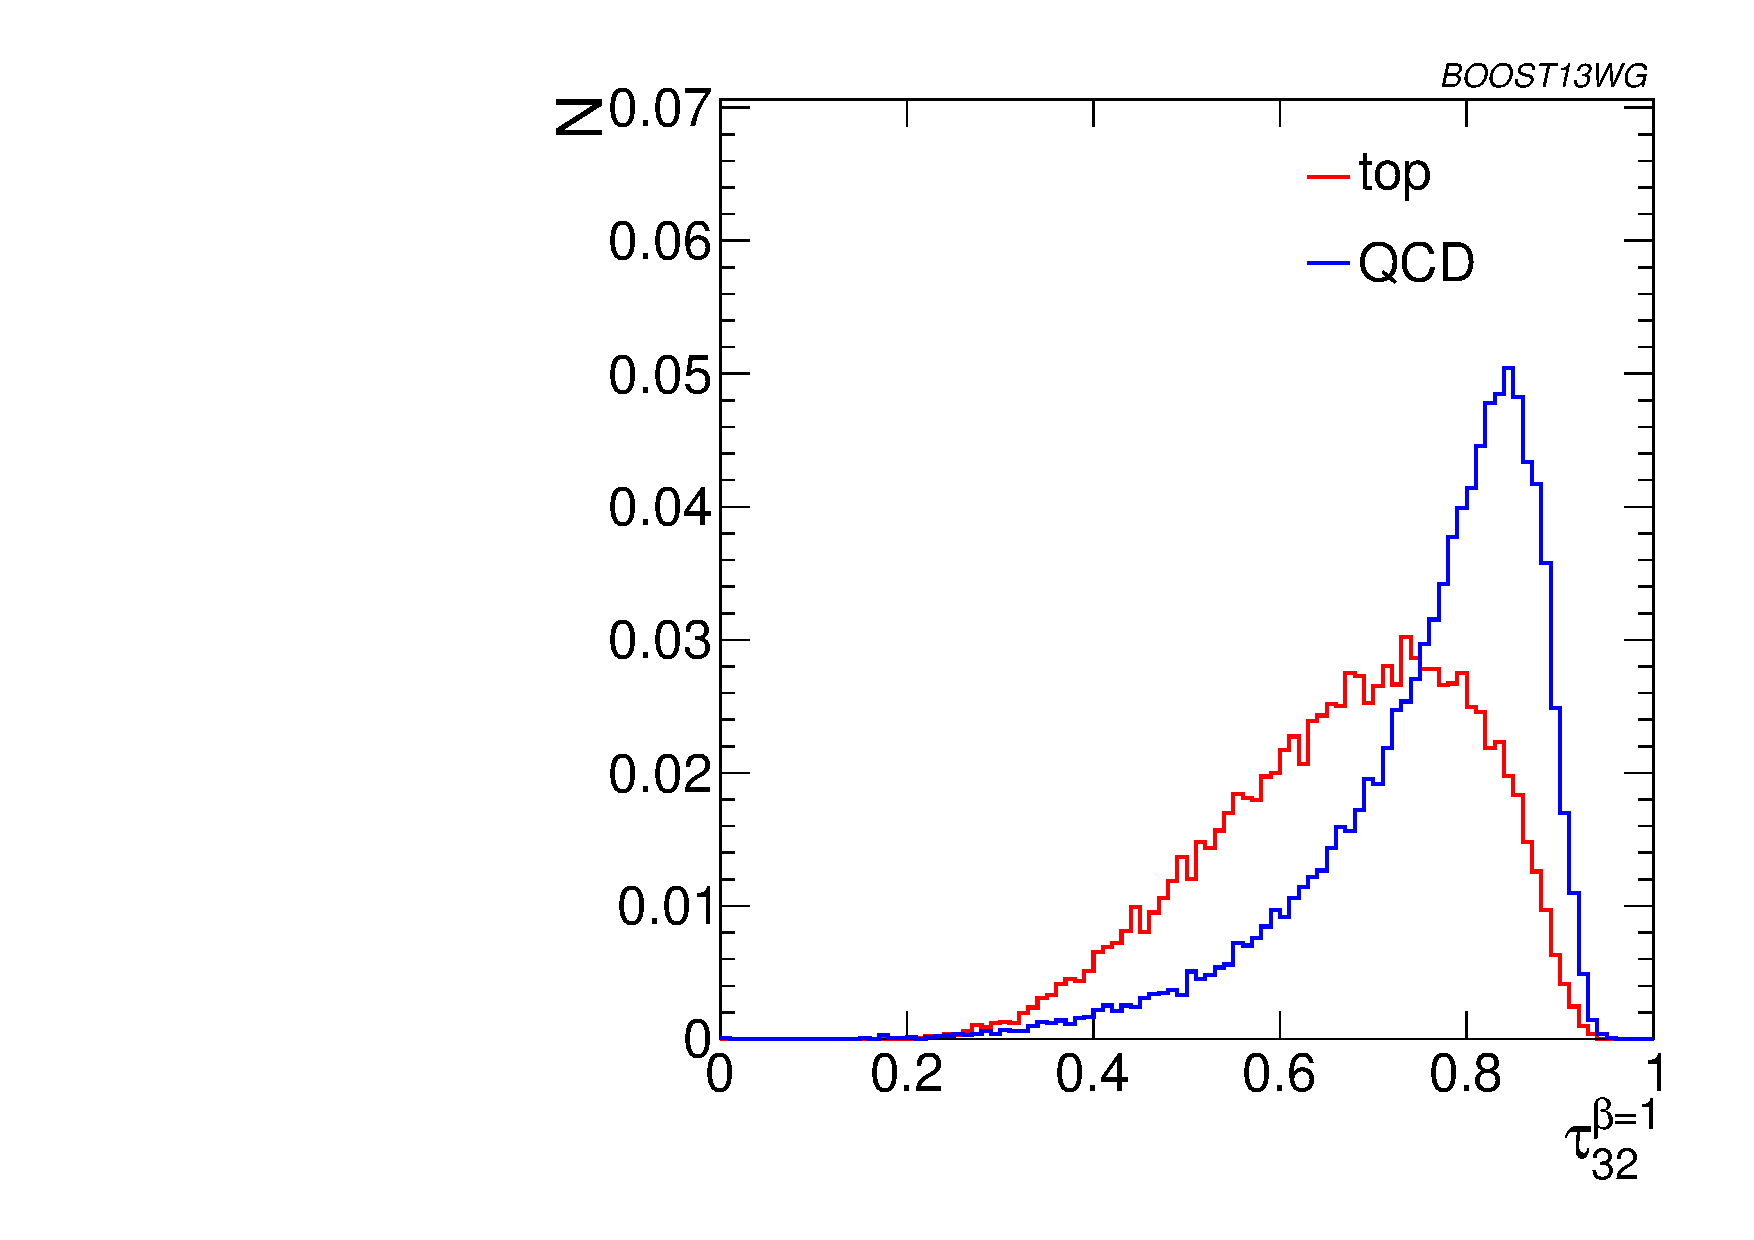
\includegraphics[width=0.32\textwidth]{./Figures/TTagging/single_variable/pT.1.5TeV.R.0.8/h_tau32b1_R_0_8.pdf}}
%\caption{Comparison of $\tau_{21}^{\beta=1}$ and $\tau_{32}^{\beta=1}$ with $R=0.8$ and different values of the $\pt$.}
%\label{fig:tau_comparison_pT}
%
%\end{figure*}

\begin{figure*}
\centering
\subfigure[HEPTopTagger $m_t$]{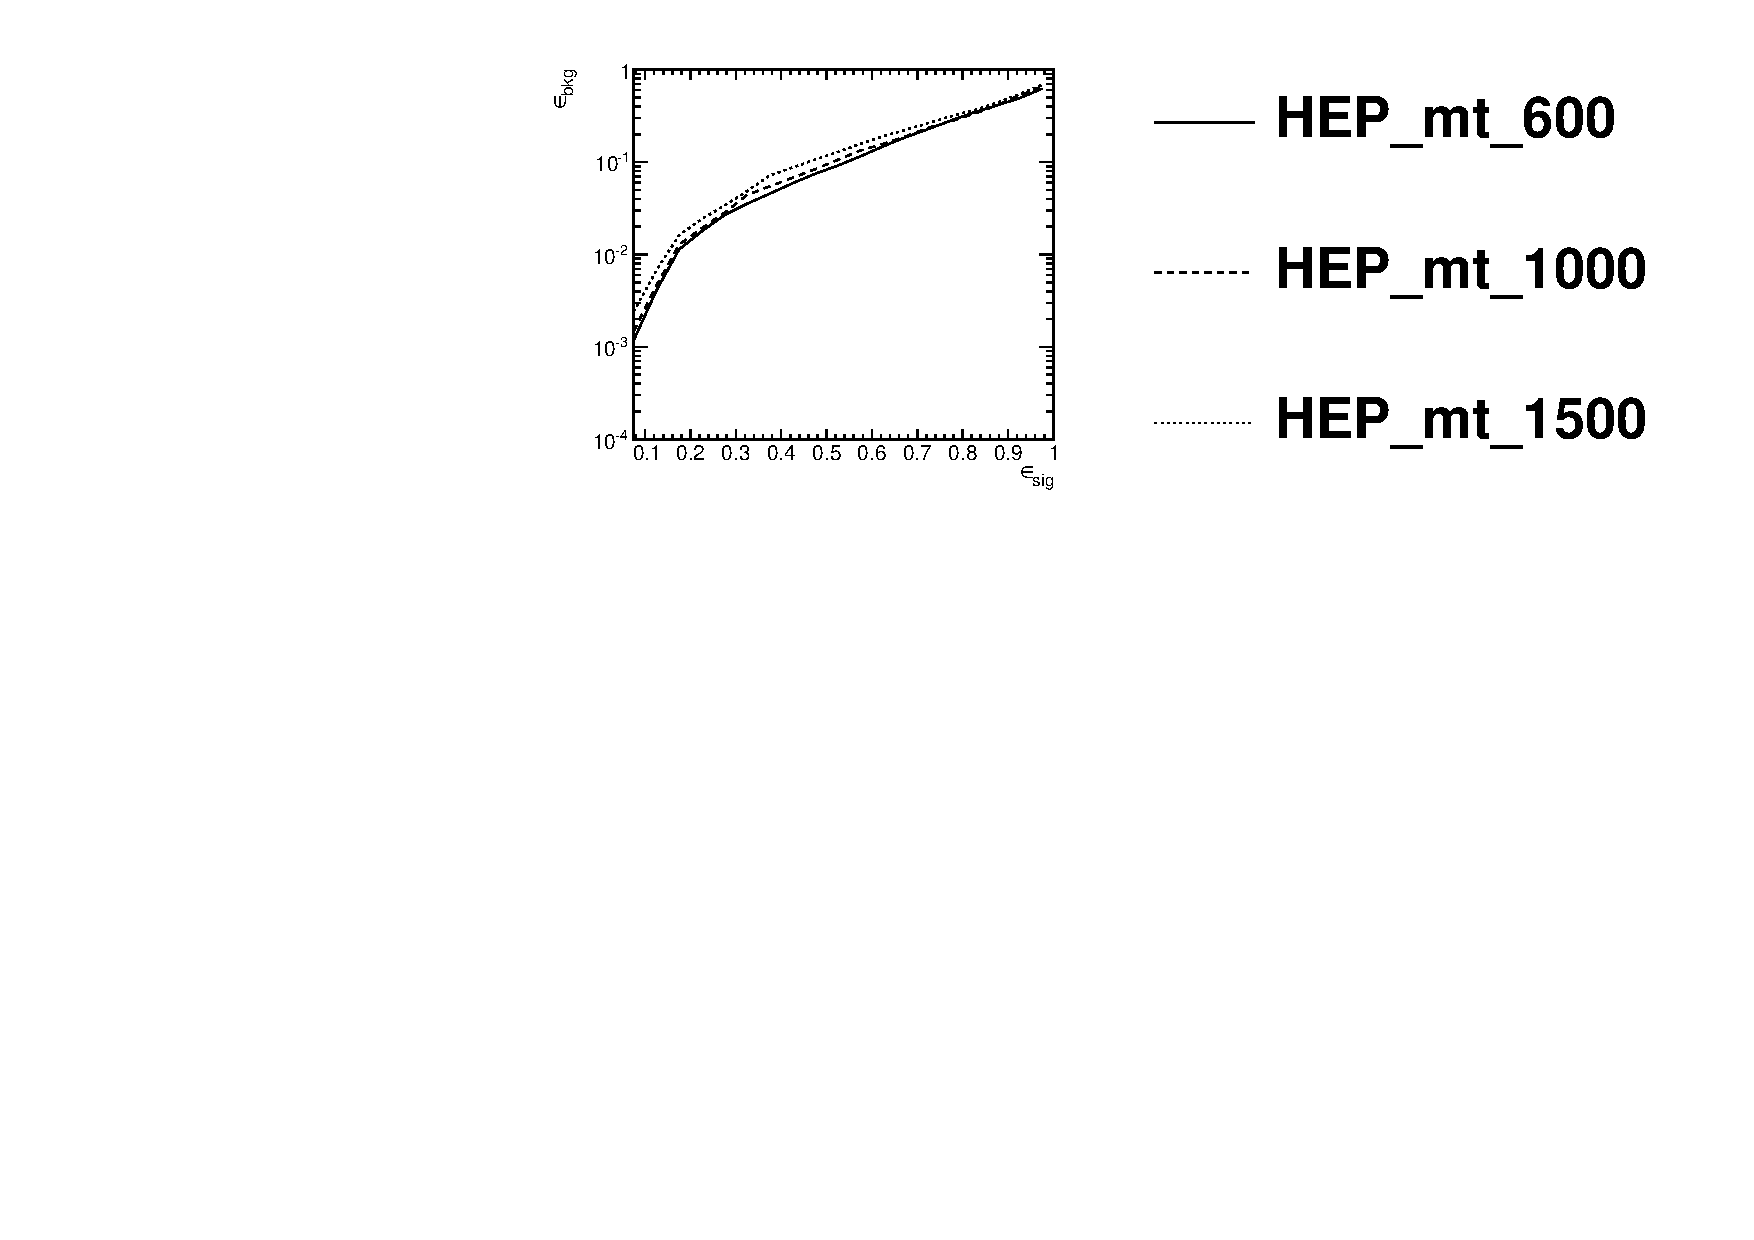
\includegraphics[width=0.48\textwidth]{./Figures/TTagging/single_variable/pT_compare/Rocs_HEP_mt_pTcompare.pdf}}
\subfigure[Johns Hopkins Tagger $m_t$]{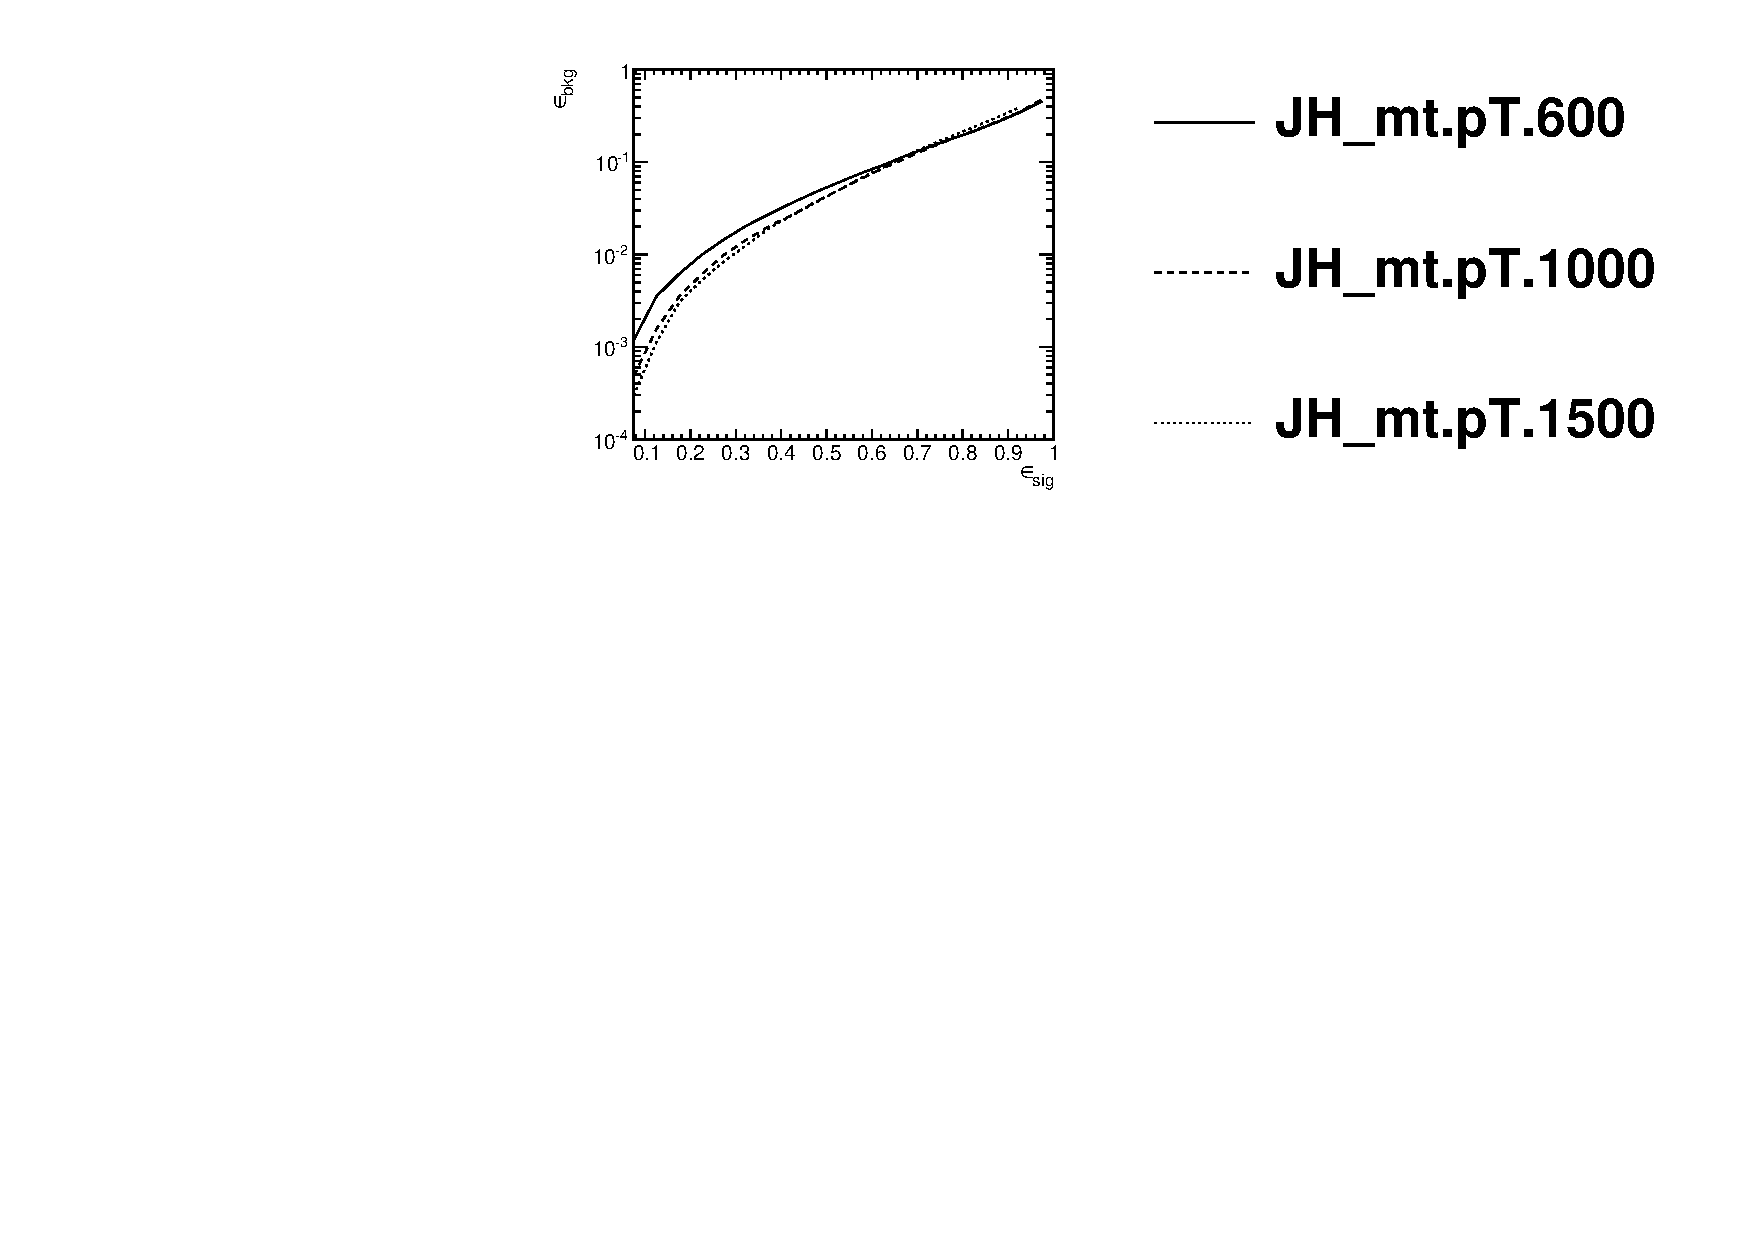
\includegraphics[width=0.48\textwidth]{./Figures/TTagging/single_variable/pT_compare/Rocs_JH_mt_pTcompare.pdf}}
\subfigure[Pruning $m_t$]{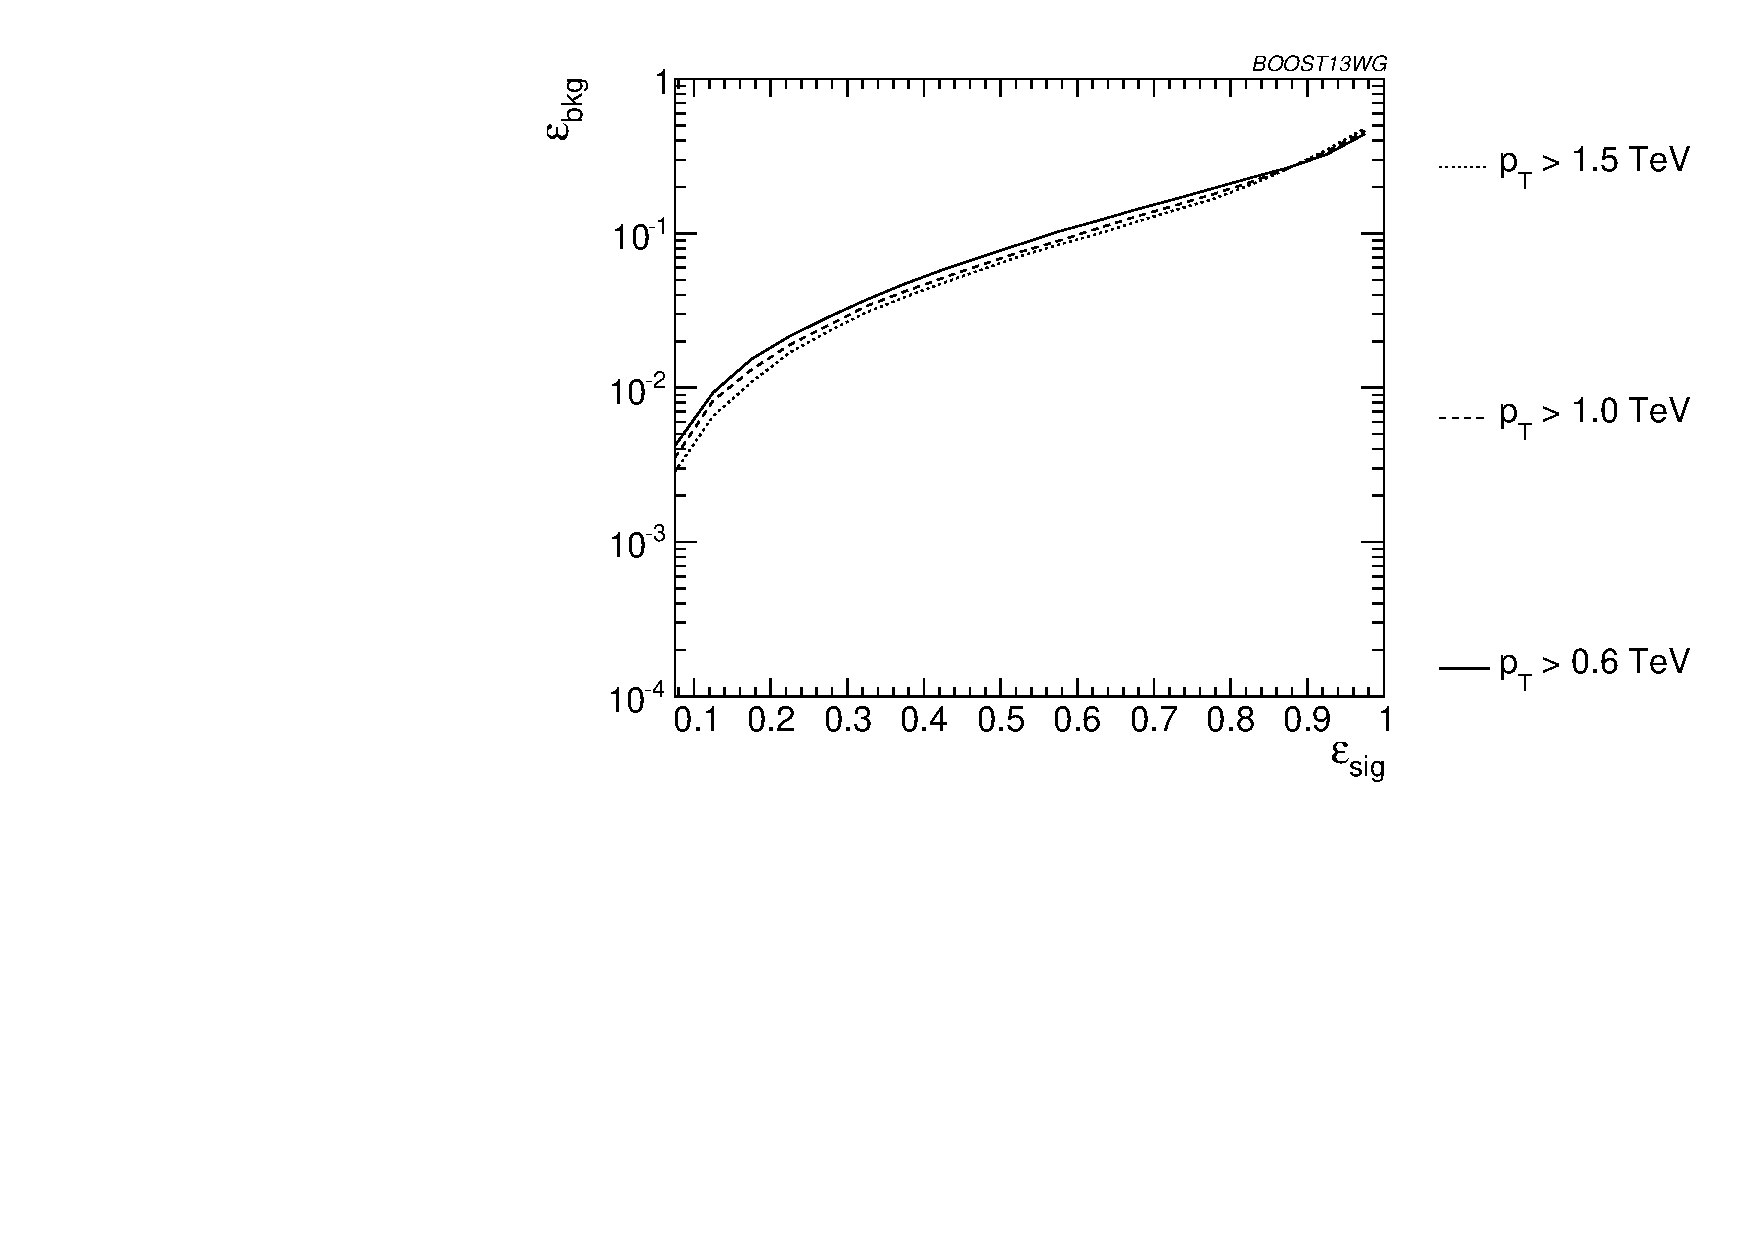
\includegraphics[width=0.48\textwidth]{./Figures/TTagging/single_variable/pT_compare/Rocs_prune_pTcompare.pdf}}
\subfigure[Trimming $m_t$]{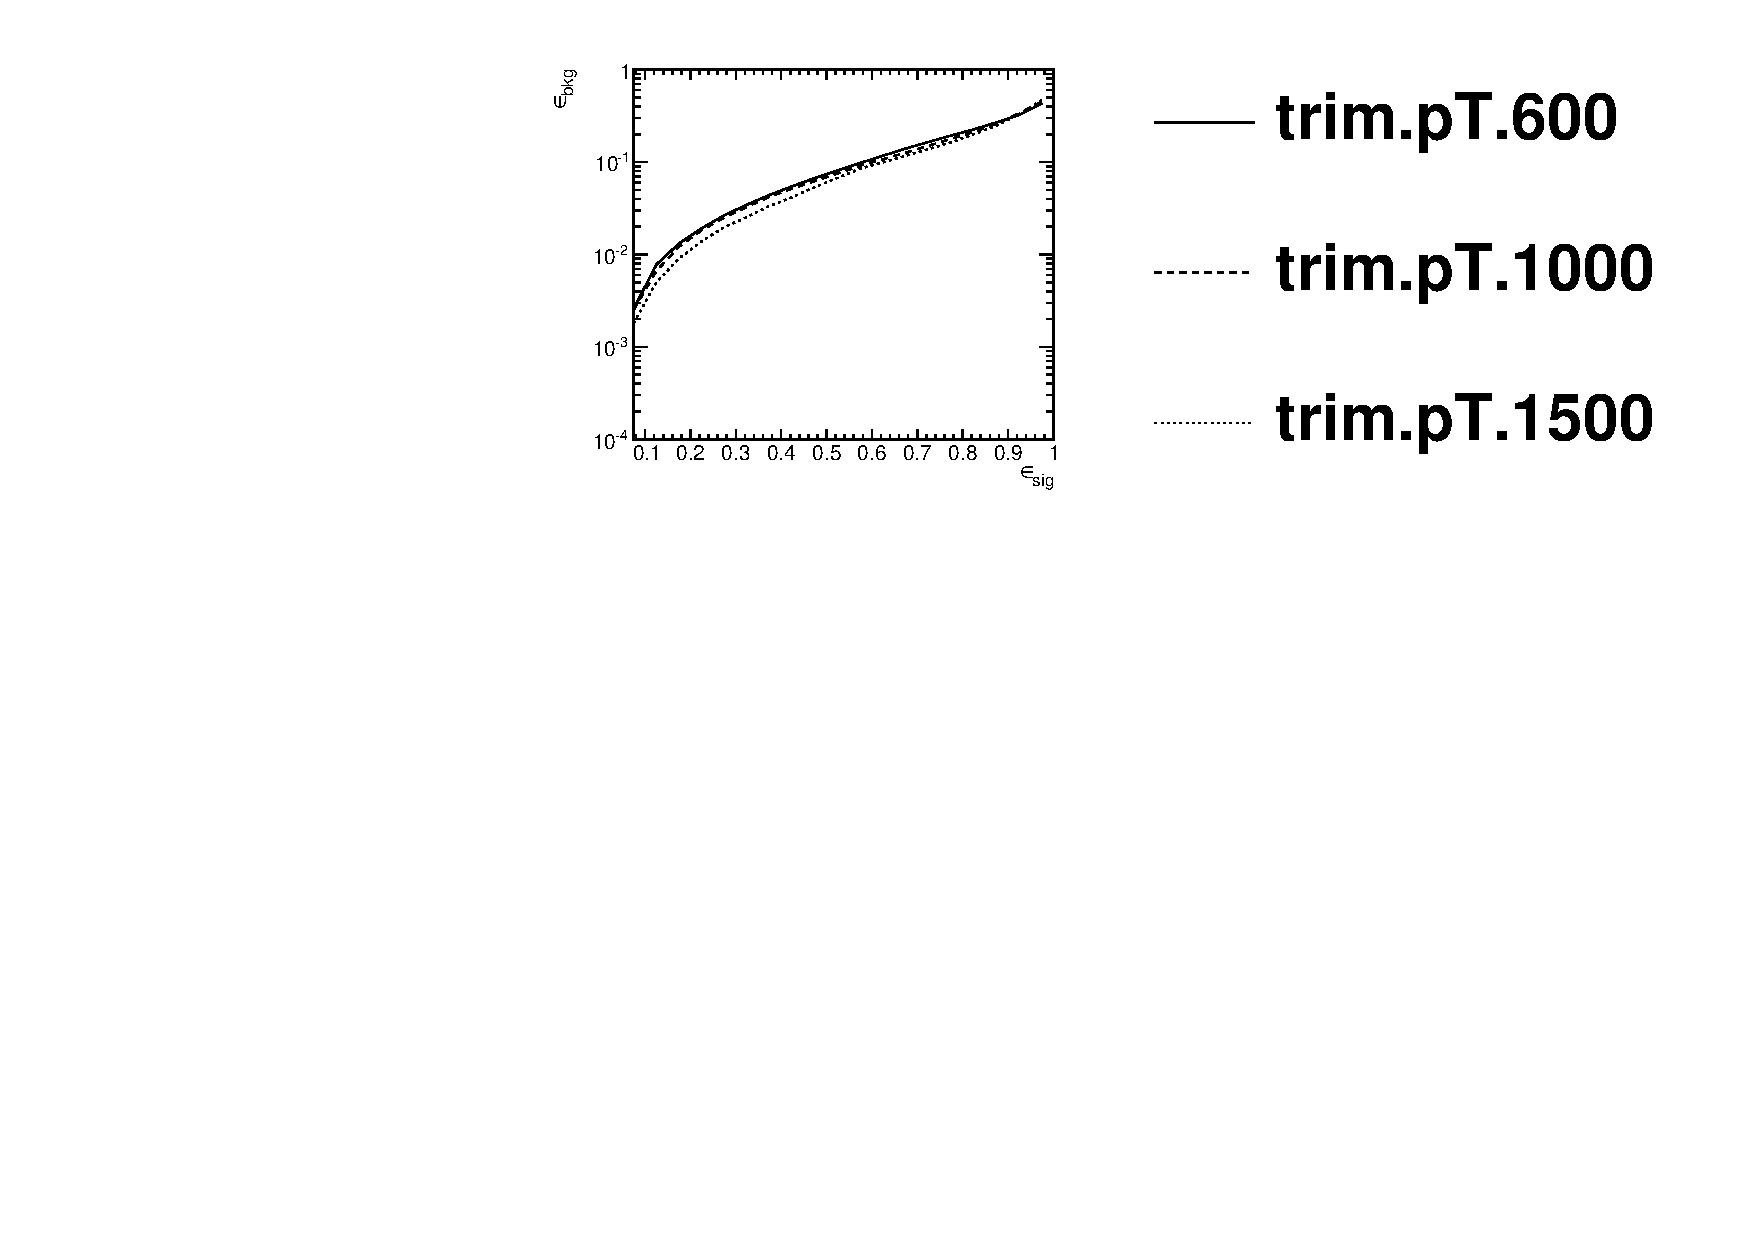
\includegraphics[width=0.48\textwidth]{./Figures/TTagging/single_variable/pT_compare/Rocs_trim_pTcompare.pdf}}
\caption{Comparison of top mass performance of different taggers at different \pt using the anti-\kT R=0.8 algorithm.}
\label{fig:ptcomparison_singletopmass_top}
\end{figure*}


In Figures~\ref{fig:Rcomparison_singleshape_top} and~\ref{fig:Rcomparison_singletopmass_top} we directly compare ROC curves for jet shape observable performance and top mass performance respectively for the three different jet radii considered within the \pt 1.5-1.6 TeV bin. Again, the input parameters of the taggers, groomers and shape variables are separately optimized for each jet radius. We can see from these figures that most of the top tagging variables, both shape and reconstructed top mass, perform best for smaller radius. This is likely because, at such high $\pt$, most of the radiation from the top quark is confined within $R=0.4$, and having a larger jet radius makes the observable more susceptible to contamination from the underlying event and other uncorrelated radiation. In Figure~\ref{fig:C_comparison_R}, we compare the individual top signal and QCD background distributions for each shape variable considered in the \pt 1.5-1.6 TeV bin for the various jet radii. One can see that the distributions for both signal and background broaden with increasing $R$, degrading the discriminating power. For $C_2^{(\beta=1)}$ and $C_3^{(\beta=1)}$, the background distributions are shifted upward as well. Therefore, the discriminating power generally gets worse with increasing $R$. The main exception is   for $C_3^{(\beta=1)}$, which performs optimally at $R=0.8$; in this case, the signal and background coincidentally happen to have the same distribution around $R=0.4$, and so $R=0.8$ gives better discrimination.


%\noindent{\bf $R$ comparison:} We compare various top tagging observables for jets of different $R$ and $\pt=1.5-1.6$ TeV in Figs.~\ref{fig:Rcomparison_singleshape_top}-\ref{fig:Rcomparison_singletopmass_top}. Most of the top-tagging parameters perform best for smaller radius; this is because, at such high $\pt$, most of the radiation from the top quark is confined within $R=0.4$, and having a larger jet radius makes the observable more susceptible to contamination from the underlying event and other uncorrelated radiation. As we show in Figs.~\ref{fig:C_comparison_R}-\ref{fig:tau_comparison_R}, the distributions for both signal broaden with increasing $R$, degrading the discriminating power. For $C_2^{(\beta=1)}$ and $C_3^{(\beta=1)}$, the background distributions are shifted upward as well. Therefore, the discriminating power generally gets worse with increasing $R$. The main exception is   for $C_3^{(\beta=1)}$, which performs optimally at $R=0.8$; in this case, the signal and background coincidentally happen to have the same distribution around $R=0.4$, and so $R=0.8$ gives better discrimination.

\begin{figure*}
\centering
\subfigure[$C_2^{(\beta=1)}$]{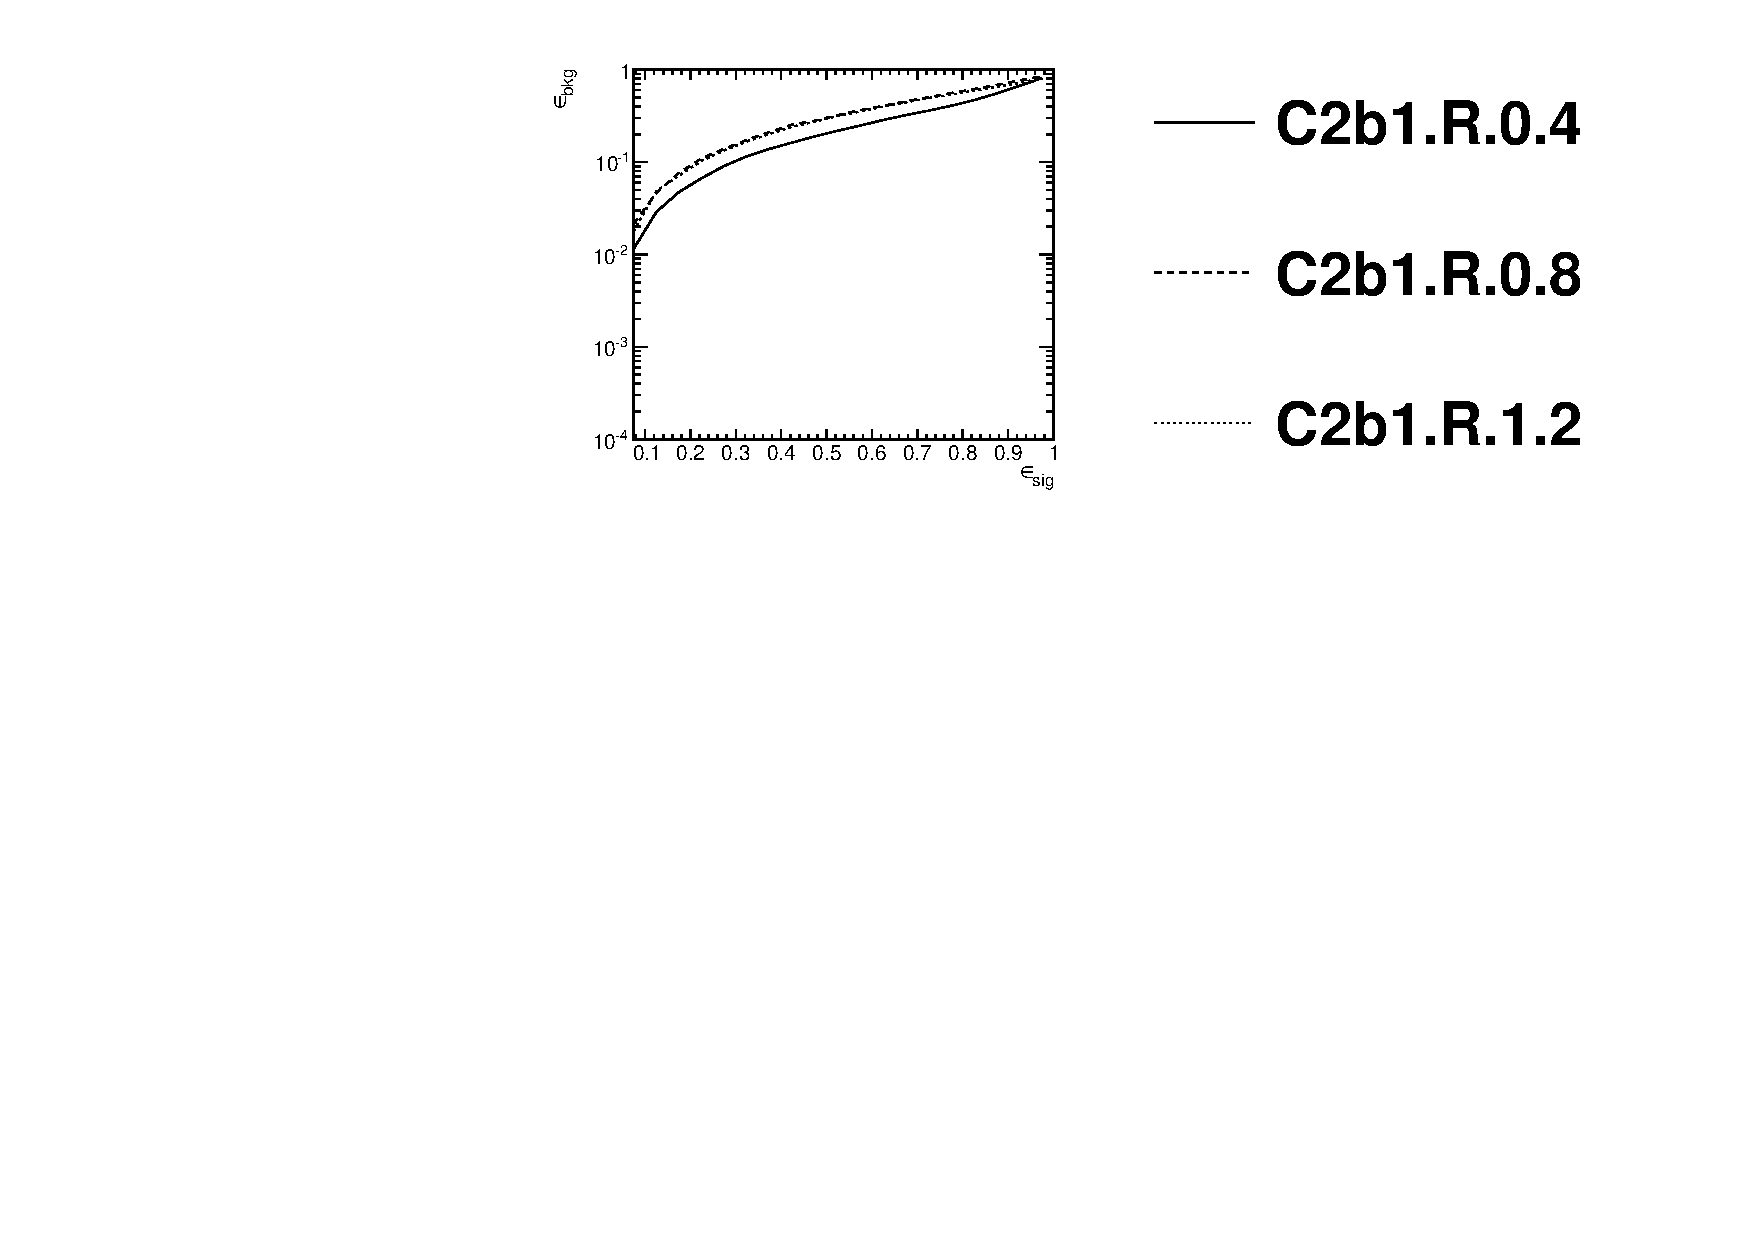
\includegraphics[width=0.48\textwidth]{./Figures/TTagging/single_variable/R_compare/Rocs_C2b1_Rcompare.pdf}}
\subfigure[$C_3^{(\beta=1)}$]{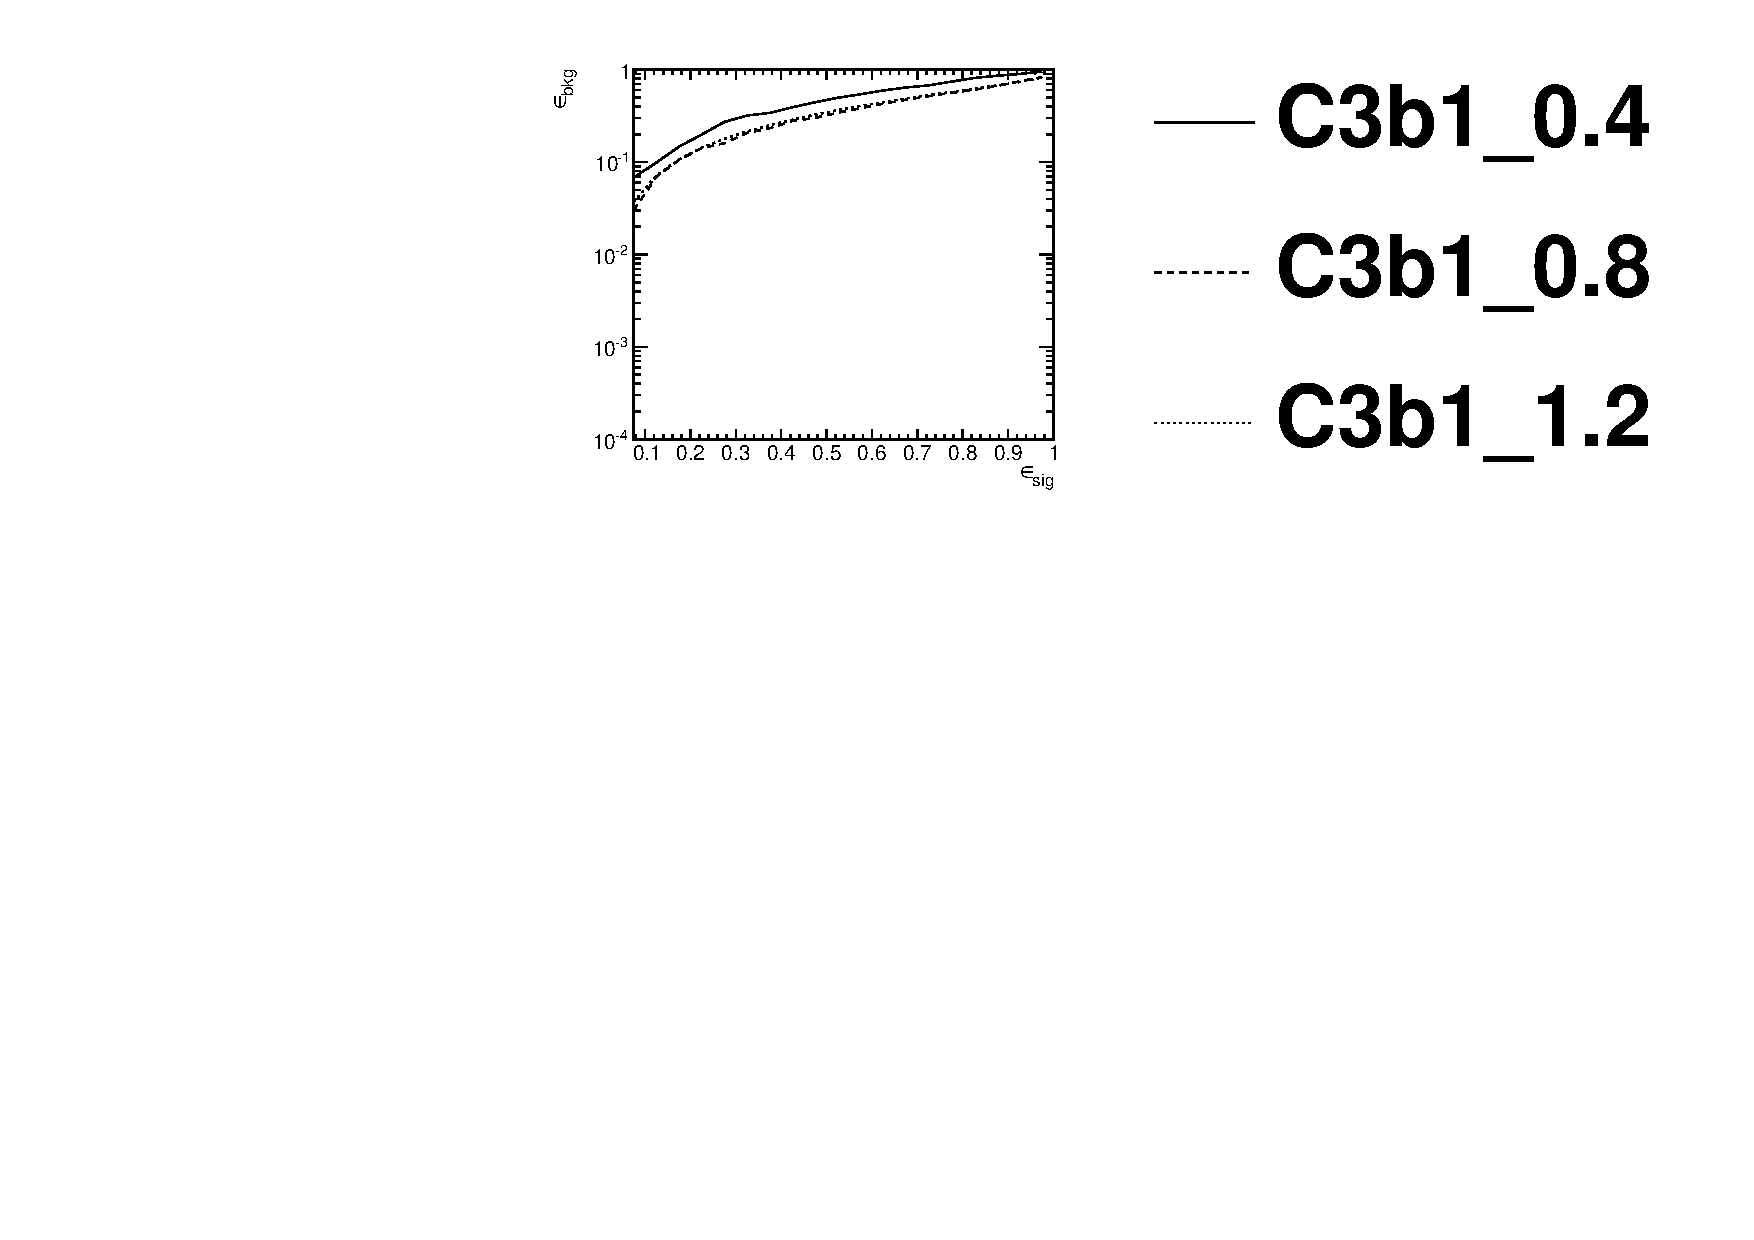
\includegraphics[width=0.48\textwidth]{./Figures/TTagging/single_variable/R_compare/Rocs_C3b1_Rcompare.pdf}}
\subfigure[$\tau_{21}^{(\beta=1)}$]{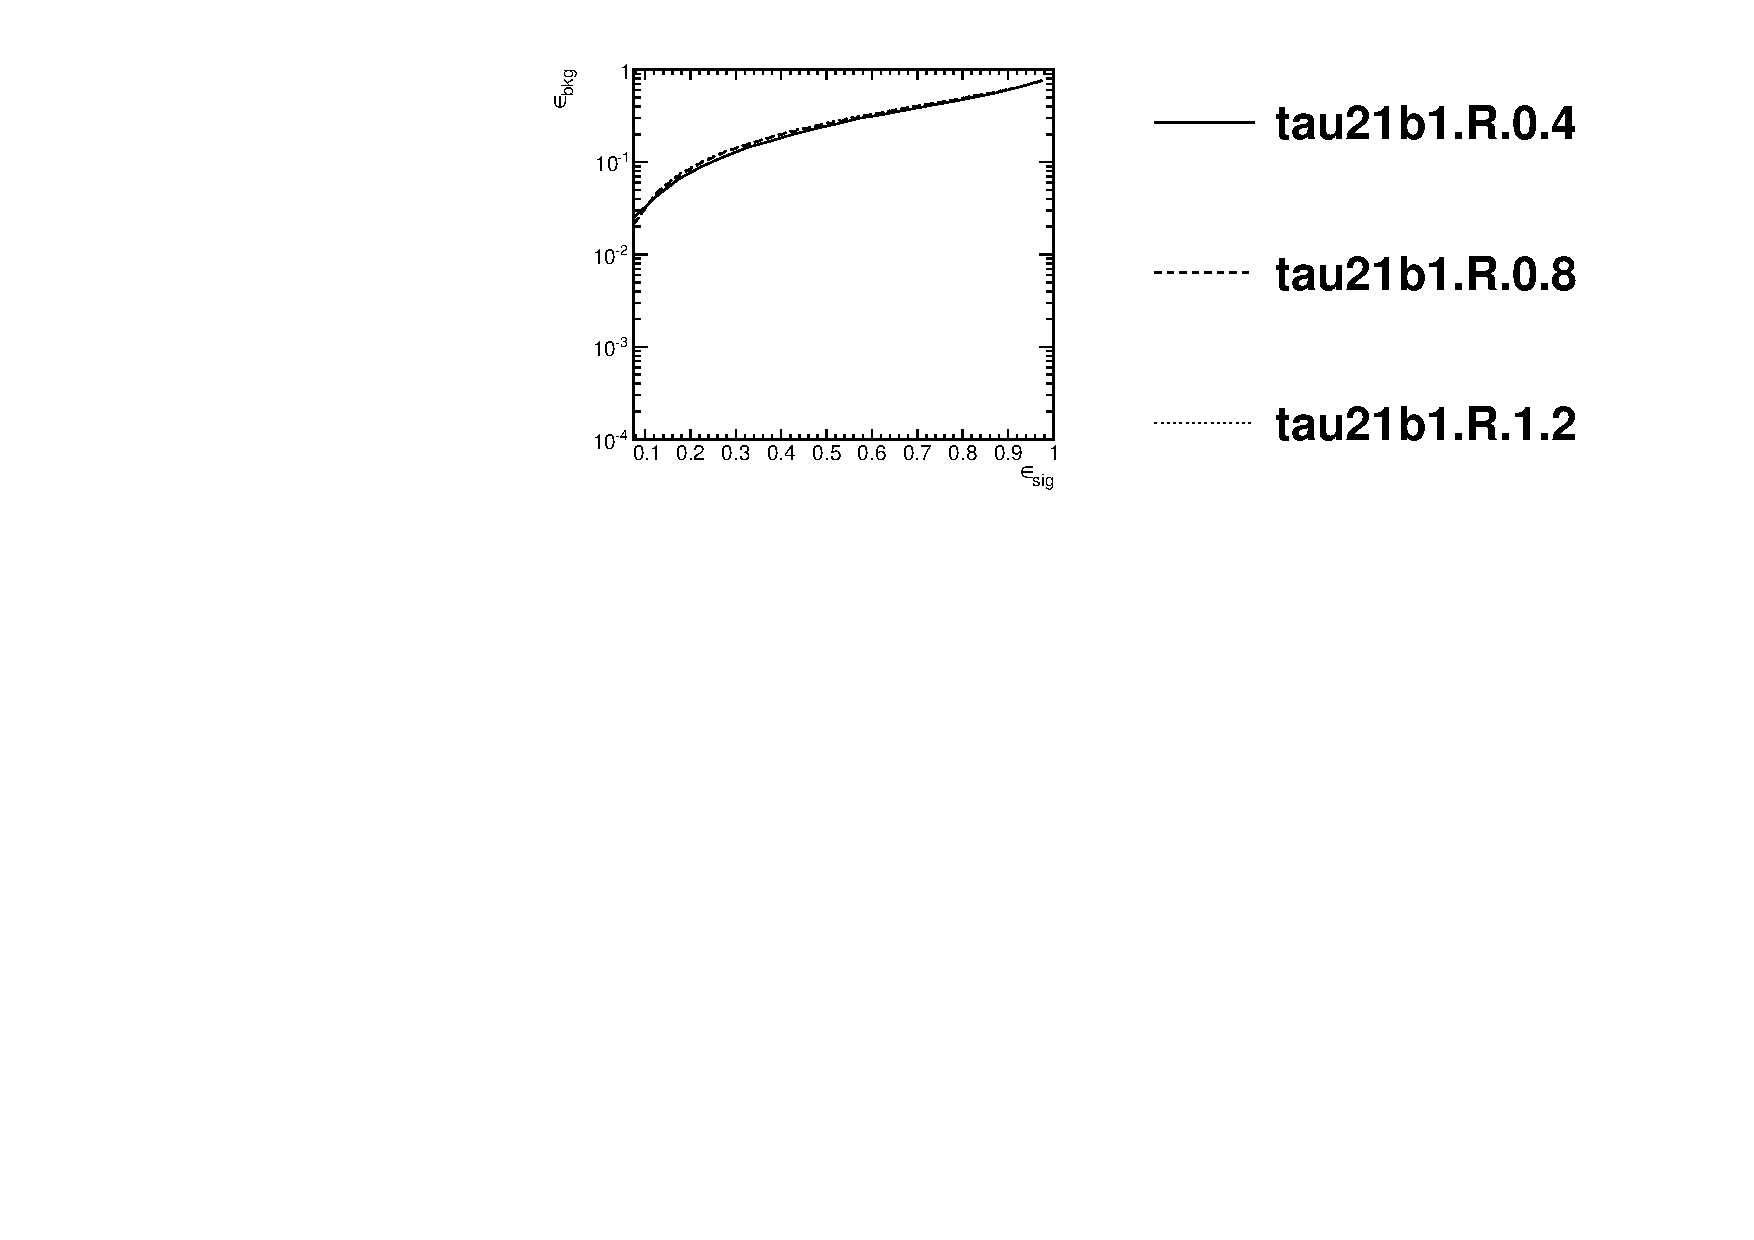
\includegraphics[width=0.48\textwidth]{./Figures/TTagging/single_variable/R_compare/Rocs_tau21b1_Rcompare.pdf}}
\subfigure[$\tau_{32}^{(\beta=1)}$]{\includegraphics[width=0.48\textwidth]{./Figures/TTagging/single_variable/R_compare/Rocs_tau32b1_Rcompare.pdf}}
\subfigure[Qjet mass volatility]{\includegraphics[width=0.48\textwidth]{./Figures/TTagging/single_variable/R_compare/Rocs_Qjet_Rcompare.pdf}}
\caption{Comparison of individual jet shape performance at different $R$ in the $\pt=1.5-1.6$ TeV bin.}
\label{fig:Rcomparison_singleshape_top}
\end{figure*}


\begin{figure*}
\centering
\subfigure[$C_2^{(\beta=1)}$, $R=0.4$]{\includegraphics[width=0.245\textwidth]{./Figures/TTagging/single_variable/pT.1.5TeV.R.0.4/h_C2B1_R_0_4.pdf}}
\subfigure[$C_2^{(\beta=1)}$, $R=1.2$]{\includegraphics[width=0.245\textwidth]{./Figures/TTagging/single_variable/pT.1.5TeV.R.1.2/h_C2B1_R_1_2.pdf}}
\subfigure[$C_3^{(\beta=1)}$, $R=0.4$]{\includegraphics[width=0.245\textwidth]{./Figures/TTagging/single_variable/pT.1.5TeV.R.0.4/h_C3B1_R_0_4.pdf}}
\subfigure[$C_3^{(\beta=1)}$, $R=1.2$]{\includegraphics[width=0.245\textwidth]{./Figures/TTagging/single_variable/pT.1.5TeV.R.1.2/h_C3B1_R_1_2.pdf}}\\
\subfigure[$\tau_{21}^{(\beta=1)}$, $R=0.4$]{\includegraphics[width=0.245\textwidth]{./Figures/TTagging/single_variable/pT.1.5TeV.R.0.4/h_tau21b1_R_0_4.pdf}}
\subfigure[$\tau_{21}^{(\beta=1)}$, $R=1.2$]{\includegraphics[width=0.245\textwidth]{./Figures/TTagging/single_variable/pT.1.5TeV.R.1.2/h_tau21b1_R_1_2.pdf}}
\subfigure[$\tau_{32}^{(\beta=1)}$, $R=0.4$]{\includegraphics[width=0.245\textwidth]{./Figures/TTagging/single_variable/pT.1.5TeV.R.0.4/h_tau32b1_R_0_4.pdf}}
\subfigure[$\tau_{32}^{(\beta=1)}$, $R=1.2$]{\includegraphics[width=0.245\textwidth]{./Figures/TTagging/single_variable/pT.1.5TeV.R.1.2/h_tau32b1_R_1_2.pdf}}\\
\subfigure[$\Gamma_{\rm Qjet}$, $R=0.4$]{\includegraphics[width=0.245\textwidth]{./Figures/TTagging/single_variable/pT.1.5TeV.R.0.4/h_qjetVol_R_0_4.pdf}}
\subfigure[$\Gamma_{\rm Qjet}$, $R=1.2$]{\includegraphics[width=0.245\textwidth]{./Figures/TTagging/single_variable/pT.1.5TeV.R.1.2/h_qjetVol_R_1_2.pdf}}
\caption{Comparison of various shape observables in the $\pt=1.5-1.6$ TeV bin and different values of the anti-$k_{\rm T}$ radius $R$.}
\label{fig:C_comparison_R}
\end{figure*}

%%\begin{figure*}
%%\centering
%\subfigure[$C_2^{(\beta=1)}$, $R=0.4$]{\includegraphics[width=0.32\textwidth]{./Figures/TTagging/single_variable/pT.1.5TeV.R.0.4/h_C2B1_R_0_4.pdf}}
%\subfigure[$C_2^{(\beta=1)}$, $R=0.8$]{\includegraphics[width=0.32\textwidth]{./Figures/TTagging/single_variable/pT.1.5TeV.R.0.8/h_C2B1_R_0_8.pdf}}
%\subfigure[$C_2^{(\beta=1)}$, $R=1.2$]{\includegraphics[width=0.32\textwidth]{./Figures/TTagging/single_variable/pT.1.5TeV.R.1.2/h_C2B1_R_1_2.pdf}}
%\subfigure[$C_3^{(\beta=1)}$, $R=0.4$]{\includegraphics[width=0.32\textwidth]{./Figures/TTagging/single_variable/pT.1.5TeV.R.0.4/h_C3B1_R_0_4.pdf}}
%\subfigure[$C_3^{(\beta=1)}$, $R=0.8$]{\includegraphics[width=0.32\textwidth]{./Figures/TTagging/single_variable/pT.1.5TeV.R.0.8/h_C3B1_R_0_8.pdf}}
%\subfigure[$C_3^{(\beta=1)}$, $R=1.2$]{\includegraphics[width=0.32\textwidth]{./Figures/TTagging/single_variable/pT.1.5TeV.R.1.2/h_C3B1_R_1_2.pdf}}
%\caption{Comparison of $C_2^{\beta=1}$ and $C_3^{\beta=1}$ in the $\pt=1.5-1.6$ TeV bin and different values of the anti-$k_{\rm T}$ radius $R$.}
%\label{fig:C_comparison_R}
%
%\end{figure*}

%\begin{figure*}
%\centering
%\subfigure[$\Gamma_{\rm Qjet}$, $R=0.4$]{\includegraphics[width=0.32\textwidth]{./Figures/TTagging/single_variable/pT.1.5TeV.R.0.4/h_qjetVol_R_0_4.pdf}}
%\subfigure[$\Gamma_{\rm Qjet}$, $R=0.8$]{\includegraphics[width=0.32\textwidth]{./Figures/TTagging/single_variable/pT.1.5TeV.R.0.8/h_qjetVol_R_0_8.pdf}}
%\subfigure[$\Gamma_{\rm Qjet}$, $R=1.2$]{\includegraphics[width=0.32\textwidth]{./Figures/TTagging/single_variable/pT.1.5TeV.R.1.2/h_qjetVol_R_1_2.pdf}}
%\caption{Comparison of $\Gamma_{\rm Qjet}$ in the $\pt=1.5-1.6$ TeV bin and different values of the anti-$k_{\rm T}$ radius $R$.}
%\label{fig:Qjet_comparison_R}
%
%\end{figure*}

%\begin{figure*}
%\centering
%\subfigure[$\tau_{21}^{(\beta=1)}$, $R=0.4$]{\includegraphics[width=0.32\textwidth]{./Figures/TTagging/single_variable/pT.1.5TeV.R.0.4/h_tau21b1_R_0_4.pdf}}
%\subfigure[$\tau_{21}^{(\beta=1)}$, $R=0.8$]{\includegraphics[width=0.32\textwidth]{./Figures/TTagging/single_variable/pT.1.5TeV.R.0.8/h_tau21b1_R_0_8.pdf}}
%\subfigure[$\tau_{21}^{(\beta=1)}$, $R=1.2$]{\includegraphics[width=0.32\textwidth]{./Figures/TTagging/single_variable/pT.1.5TeV.R.1.2/h_tau21b1_R_1_2.pdf}}
%\subfigure[$\tau_{32}^{(\beta=1)}$, $R=0.4$]{\includegraphics[width=0.32\textwidth]{./Figures/TTagging/single_variable/pT.1.5TeV.R.0.4/h_tau32b1_R_0_4.pdf}}
%\subfigure[$\tau_{32}^{(\beta=1)}$, $R=1.8$]{\includegraphics[width=0.32\textwidth]{./Figures/TTagging/single_variable/pT.1.5TeV.R.0.8/h_tau32b1_R_0_8.pdf}}
%\subfigure[$\tau_{32}^{(\beta=1)}$, $R=1.2$]{\includegraphics[width=0.32\textwidth]{./Figures/TTagging/single_variable/pT.1.5TeV.R.1.2/h_tau32b1_R_1_2.pdf}}
%\caption{Comparison of $\tau_{21}^{\beta=1}$ and $\tau_{32}^{\beta=1}$ in the $\pt=1.5-1.6$ TeV bin and different values of the anti-$k_{\rm T}$ radius $R$.}
%\label{fig:tau_comparison_R}
%
%\end{figure*}


\begin{figure*}
\centering
\subfigure[HEPTopTagger $m_t$]{\includegraphics[width=0.48\textwidth]{./Figures/TTagging/single_variable/R_compare/Rocs_HEP_mt_Rcompare.pdf}}
\subfigure[Johns Hopkins Tagger $m_t$]{\includegraphics[width=0.48\textwidth]{./Figures/TTagging/single_variable/R_compare/Rocs_JH_mt_Rcompare.pdf}}
\subfigure[Pruning $m_t$]{\includegraphics[width=0.48\textwidth]{./Figures/TTagging/single_variable/R_compare/Rocs_prune_Rcompare.pdf}}
\subfigure[Trimming $m_t$]{\includegraphics[width=0.48\textwidth]{./Figures/TTagging/single_variable/R_compare/Rocs_trim_Rcompare.pdf}}
\caption{Comparison of top mass performance of different taggers at different $R$ in the $\pt=1.5-1.6$ TeV bin.}
\label{fig:Rcomparison_singletopmass_top}
\end{figure*}


\subsection{Performance of multivariable combinations}
We now consider various BDT combinations of the observables from Section \ref{sec:single_variable}, using the techniques described in Section~\ref{sec:multivariate}. In particular, we consider the performance of individual taggers such as the JH tagger and HEPTopTagger, which output information about the top  and $W$ candidate masses and the helicity angle; groomers, such as trimming and pruning, which remove soft, uncorrelated radiation from the top candidate to improve mass reconstruction, and to which we have added a $W$ reconstruction step; and the combination of the outputs of the above taggers/groomers, both with each other, and with shape variables such as $N$-subjettiness ratios and energy correlation ratios. For all observables with tuneable input parameters, we scan and optimize over realistic values of such parameters, as described in Section~\ref{sec:topmethod}.



In Figure~\ref{fig:pt1000_allcompare_AKt_R08_TG}, we directly compare the performance of the HEPTopTagger, the JH tagger, trimming, and pruning, in the $\pt = 1-1.1$ TeV bin using jet radius R=0.8, where both \topmass and \wmass are used in the groomers. Generally, we find that pruning, which does not naturally incorporate subjets into the algorithm, does not perform as well as the others. Interestingly, trimming, which does include a subjet-identification step, performs comparably to the HEPTopTagger over much of the range, possibly due to the background-shaping observed in Section \ref{sec:single_variable}. By contrast, the JH tagger outperforms the other algorithms. To determine whether there is complementary information in the mass outputs from different top taggers, we also consider in Figure~\ref{fig:pt1000_allcompare_AKt_R08_TG} a multivariable combination of all of the JH and HEPTopTagger outputs. The maximum efficiency of the combined JH and HEPTopTaggers is limited, as some fraction of signal events inevitably fails either one or other of the taggers. We do see a 20-50\% improvement in performance when combining all outputs, which suggests that the different algorithms used to identify the top and $W$ for different taggers contains complementary information.

\begin{figure*}
\centering
{\includegraphics[width=0.68\textwidth]{./Figures/TTagging/multi_variable/pT.1TeV.R.0.8/Rocs_tagger_groom.pdf}}
\caption{The performance of the various taggers in the $\pt = 1-1.1$ TeV bin using the anti-\kT R=0.8 algorithm. For the groomers a BDT combination of the reconstructed \topmass and \wmass are used. Also shown is a multivariable combination of all of the JH and HEPTopTagger outputs. The ungroomed mass performance is shown for comparison.}
\label{fig:pt1000_allcompare_AKt_R08_TG}
\end{figure*}


In Figure~\ref{fig:pt1000_allcompare_AKt_R08_TagSh} we present the results for multivariable combinations of the top tagger outputs with and without shape variables. We see that, for both the HEPTopTagger and the JH tagger, the shape observables contain additional information uncorrelated with the masses and helicity angle, and give on average a factor 2-3 improvement in signal discrimination. We see that, when combined with the tagger outputs, both the energy correlation functions $C_2+C_3$ and the $N$-subjettiness ratios $\tau_{21}+\tau_{32}$ give comparable performance, while the Qjet mass volatility is slightly worse; this is unsurprising, as Qjets accesses shape information in a more indirect way from other shape observables. Combining all shape observables with a single top tagger provides even greater enhancement in discrimination power. We directly compare the performance of the JH and HEPTopTaggers in Figure~\ref{fig:pt1000_allcompare_AKt_R08_TagSh_Comp}. Combining the taggers with shape information nearly erases the difference between the tagging methods observed in Figure~\ref{fig:pt1000_allcompare_AKt_R08_TG}; this indicates that combining the shape information with the HEPTopTagger identifies the differences between signal and background missed by the tagger alone. This also suggests that further improvement to discriminating power may be minimal, as various multivariable combinations are converging to within a factor of 20\% or so.


\begin{figure*}
\centering
\subfigure[HEPTopTagger + Shape]{\includegraphics[width=0.48\textwidth]{./Figures/TTagging/multi_variable/pT.1TeV.R.0.8/Rocs_HEP.pdf}}
\subfigure[Johns Hopkins Tagger + shape]{\includegraphics[width=0.48\textwidth]{./Figures/TTagging/multi_variable/pT.1TeV.R.0.8/Rocs_JH.pdf}}
\subfigure[HEP vs.~JH comparison (incl. shape)]{\includegraphics[width=0.48\textwidth]{./Figures/TTagging/multi_variable/pT.1TeV.R.0.8/Rocs_tagger_shape.pdf}\label{fig:pt1000_allcompare_AKt_R08_TagSh_Comp}}
\caption{The performance of BDT combinations of the JH and HepTopTagger outputs with various shape observables in the $\pt = 1-1.1$ TeV bin using the anti-\kT R=0.8 algorithm. Taggers are combined with the following shape observables: $\tau_{21}^{(\beta=1)}+\tau_{32}^{(\beta=1)}$, $C_{2}^{(\beta=1)}+C_{3}^{(\beta=1)}$, $\Gamma_{\rm Qjet}$, and all of the above (denoted ``shape'').}
\label{fig:pt1000_allcompare_AKt_R08_TagSh}
\end{figure*}

In Figure~\ref{fig:pt1000_allcompare_AKt_R08_GroomSh} we present the results for multivariable combinations of groomer outputs with and without shape variables. As with the tagging algorithms, combinations of groomers with shape observables improves their discriminating power; combinations with $\tau_{32}+\tau_{21}$ perform comparably to those with $C_3+C_2$, and both of these are superior to combinations with the mass volatility, $\Gamma$. Substantial improvement is further possible by combining the groomers with all shape observables. Not surprisingly, the taggers that lag behind in performance enjoy the largest gain in signal-background discrimination with the addition of shape observables. Once again, in Figure~\ref{fig:pt1000_allcompare_AKt_R08_GroomSh_Comp}, we find that the differences between pruning and trimming are erased when combined with shape information.

\begin{figure*}
\centering
\subfigure[Pruning + Shape]{\includegraphics[width=0.48\textwidth]{./Figures/TTagging/multi_variable/pT.1TeV.R.0.8/Rocs_prune.pdf}}
\subfigure[Trimming + Shape]{\includegraphics[width=0.48\textwidth]{./Figures/TTagging/multi_variable/pT.1TeV.R.0.8/Rocs_trim.pdf}}
\subfigure[Trim vs.~Prune comparison (incl. shape)]{\includegraphics[width=0.48\textwidth]{./Figures/TTagging/multi_variable/pT.1TeV.R.0.8/Rocs_groom_shape.pdf}\label{fig:pt1000_allcompare_AKt_R08_GroomSh_Comp}}
\caption{The performance of the BDT combinations of the trimming and pruning outputs with various shape observables in the $\pt = 1-1.1$ TeV bin using the anti-\kT R=0.8 algorithm. Groomer mass outputs are combined with the following shape observables: $\tau_{21}^{(\beta=1)}+\tau_{32}^{(\beta=1)}$, $C_{2}^{(\beta=1)}+C_{3}^{(\beta=1)}$, $\Gamma_{\rm Qjet}$, and all of the above (denoted ``shape'').}
\label{fig:pt1000_allcompare_AKt_R08_GroomSh}
\end{figure*}

Finally, in Figure~\ref{fig:pt1000_allcompare_AKt_R08_Final}, we compare the performance of each of the tagger/groomers when their outputs are combined with all of the shape observables considered. One can see that the discrepancies between the performance of the different taggers/groomers all but vanishes, suggesting perhaps that we are here utilising all available signal-background discrmination information, and that this is the optimal top tagging performance that could be achieved in these conditions. 

\begin{figure*}
\centering
{\includegraphics[width=0.68\textwidth]{./Figures/TTagging/multi_variable/pT.1TeV.R.0.8/Rocs_optimum.pdf}}
\caption{Comparison of the performance of the BDT combinations of all the groomer/tagger outputs with all the available shape observables in the $\pt = 1-1.1$ TeV bin using the anti-\kT R=0.8 algorithm. Tagger/groomer outputs are combined with all of the following shape observables: $\tau_{21}^{(\beta=1)}+\tau_{32}^{(\beta=1)}$, $C_{2}^{(\beta=1)}+C_{3}^{(\beta=1)}$, $\Gamma_{\rm Qjet}$.}
\label{fig:pt1000_allcompare_AKt_R08_Final}
\end{figure*}

%In Figure~\ref{fig:pt1000_allcompare_AKt_R08} are shown ROC curves which summarise the results for the multivariable combinations, using jet radius 0.8 in the \pt 1.0-1.1 TeV bin; in all cases, we also show the ungroomed jet mass as a baseline comparison. In Figure~\ref{fig:pt1000_allcompare_AKt_R08_TG}, we directly compare the performance of the HEPTopTagger, the JH tagger, trimming, and pruning, where both \topmass and \wmass are used in the groomers. Generally, we find that pruning, which does not naturally incorporate subjets into the algorithm, does not perform as well as the others. Interestingly, trimming, which does include a subjet-identification step, performs comparably to the HEPTopTagger over much of the range, possibly due to the background-shaping observed in Section \ref{sec:single_variable}. By contrast, the JH tagger outperforms the other algorithms. To determine whether there is complementary information in the mass outputs from different top taggers, we also consider in Figure~\ref{fig:pt1000_allcompare_AKt_R08_TG} a multivariable combination of all of the JH and HEPTopTagger outputs. The maximum efficiency of the combined JH and HEPTopTaggers is limited, as some fraction of signal events inevitably fails either one or other of the taggers. We do see a 20-50\% improvement in performance when combining all outputs, which suggests that the different algorithms used to identify the top and $W$ for different taggers contains complementary information.

%In Fig.~\ref{fig:pt1000_allcompare_AKt_R08}(b)-(d), we present the results for multivariable combinations of top tagger outputs with and without shape variables. We see that, for both the HEPTopTagger and the JH tagger, the shape observables contain additional information uncorrelated with the masses and helicity angle, and give on average 2-3 improvement in signal discrimination. We see that, when combined with the tagger outputs, both the energy correlation functions $C_2+C_3$ and the $N$-subjettiness ratios $\tau_{21}+\tau_{32}$ give comparable performance, while the Qjet mass volatility is slightly worse; this is unsurprising, as Qjets accesses shape information in a more indirect way from other shape observables. Combining all shape observables with a single top tagger provides  even more  enhancement in discrimination power.

%We directly compare the performance of the JH and HEPTopTaggers in Fig.~\ref{fig:pt1000_allcompare_AKt_R08}(d). Combining the taggers with shape information nearly erases the difference between the tagging methods observed in Fig.~\ref{fig:pt1000_allcompare_AKt_R08}(a); this indicates that combining the shape information with the HEPTopTagger identifies the differences between signal and background missed by the tagger alone. This also suggests that further improvement to discriminating power may be minimal, as various multivariable combinations are converging to within a factor of 20\% or so.

%In Fig.~\ref{fig:pt1000_allcompare_AKt_R08}(e)-(g), we present the results for multivariable combinations of groomer outputs with and without shape variables. As with the tagging algorithms, combinations of groomers with shape observables improves their discriminating power; combinations with $\tau_{32}+\tau_{21}$ perform comparably to those with $C_3+C_2$, and both of these are superior to combinations with the mass volatility, $\Gamma$. Substantial improvement is further possible by combining the groomers with all shape observables. Not surprisingly, the taggers that lag behind in performance enjoy the largest gain in signal-background discrimination with the addition of shape observables. Once again, in \ref{fig:pt1000_allcompare_AKt_R08}(g), we find that the differences between pruning and trimming are erased when combined with shape information.\\


%\begin{figure*}
%\centering
%\subfigure[Tagger-Groomer comparison]{\includegraphics[width=0.48\textwidth]{./Figures/TTagging/multi_variable/pT.1TeV.R.0.8/Rocs_tagger_groom.pdf}\label{fig:pt1000_allcompare_AKt_R08_TG}}
%\subfigure[HEPTopTagger + Shape]{\includegraphics[width=0.48\textwidth]{./Figures/TTagging/multi_variable/pT.1TeV.R.0.8/Rocs_HEP.pdf}}
%\subfigure[Johns Hopkins Tagger + shape]{\includegraphics[width=0.48\textwidth]{./Figures/TTagging/multi_variable/pT.1TeV.R.0.8/Rocs_JH.pdf}}
%\subfigure[HEP vs.~JH comparison (incl. shape)]{\includegraphics[width=0.48\textwidth]{./Figures/TTagging/multi_variable/pT.1TeV.R.0.8/Rocs_tagger_shape.pdf}}
%\subfigure[Pruning + Shape]{\includegraphics[width=0.48\textwidth]{./Figures/TTagging/multi_variable/pT.1TeV.R.0.8/Rocs_prune.pdf}}
%\subfigure[Trimming + Shape]{\includegraphics[width=0.48\textwidth]{./Figures/TTagging/multi_variable/pT.1TeV.R.0.8/Rocs_trim.pdf}}
%\subfigure[Trim vs.~Prune comparison (incl. shape)]{\includegraphics[width=0.48\textwidth]{./Figures/TTagging/multi_variable/pT.1TeV.R.0.8/Rocs_groom_shape.pdf}}
%\subfigure[Comparison of all Tagger+Shape]{\includegraphics[width=0.48\textwidth]{./Figures/TTagging/multi_variable/pT.1TeV.R.0.8/Rocs_optimum.pdf}}
%\caption{The performance of the BDT combinations in the $\pt = 1-1.1$ TeV bin using the anti-\kT R=0.8 algorithm. Taggers are combined with the following shape observables: $\tau_{21}^{(\beta=1)}+\tau_{32}^{(\beta=1)}$, $C_{2}^{(\beta=1)}+C_{3}^{(\beta=1)}$, $\Gamma_{\rm Qjet}$, and all of the above (denoted ``shape'').}
%\label{fig:pt1000_allcompare_AKt_R08}
%
%\end{figure*}


Up to this point we have just considered the combined multivariable performance in the \pt 1.0-1.1 TeV bin with jet radius R=0.8. We now compare the BDT combinations of tagger outputs, with and without shape variables, at different $\pt$. The taggers are optimized over all input parameters for each choice of \pt and signal efficiency. As with the single-variable study, we consider anti-$k_{\rm T}$ jets clustered with $R=0.8$ and compare the outcomes in the $\pt=500-600$ GeV, $\pt=1-1.1$ TeV, and $\pt=1.5-1.6$ TeV bins. The comparison of the taggers/groomers is shown in Figure~\ref{fig:ptcomparison_top}. The behaviour with \pt is qualitatively similar to the behaviour of the \topmass observable for each tagger/groomer shown in Figure~\ref{fig:ptcomparison_singletopmass_top}; this suggests that the \pt behaviour of the taggers is dominated by the top mass reconstruction. As before, the HEPTopTagger performance degrades slightly with increased \pt due to the background shaping effect, while the JH tagger and groomers modestly improve in performance.

In Figure~\ref{fig:ptcomparison_JH_shape}, we show the $\pt$ dependence of BDT combinations of the JH tagger output combined with shape observables. We find that the curves look nearly identical: the \pt dependence is dominated by the top mass reconstruction, and combining the tagger outputs with different shape observables does not substantially change this behaviour. The same holds true for trimming and pruning. By contrast,  HEPTopTagger ROC curves, shown in Figure~\ref{fig:ptcomparison_HEP_shape}, do change somewhat when combined with different shape observables; due to the suboptimal performance of the HEPTopTagger at high \pt, we find that combining the HEPTopTagger with $C_3^{(\beta=1)}$, which in Figure~\ref{fig:ptcomparison_singleshape_top_C3} is seen to have some modest improvement at high \pt, can improve its performance. Combining the HEPTopTagger with multiple shape observables gives the maximum improvement in performance at high \pt relative to at low \pt.\\

\begin{figure*}
\centering
\subfigure[HEPTopTagger]{\includegraphics[width=0.48\textwidth]{./Figures/TTagging/multi_variable/pT_compare/Rocs_HEP_pTcompare.pdf}}
\subfigure[Johns Hopkins Tagger]{\includegraphics[width=0.48\textwidth]{./Figures/TTagging/multi_variable/pT_compare/Rocs_JH_pTcompare.pdf}}
\subfigure[Trimming]{\includegraphics[width=0.48\textwidth]{./Figures/TTagging/multi_variable/pT_compare/Rocs_trim_mt_mw_pTcompare.pdf}}
\subfigure[Pruning]{\includegraphics[width=0.48\textwidth]{./Figures/TTagging/multi_variable/pT_compare/Rocs_prune_mt_mw_pTcompare.pdf}}
\caption{Comparison of BDT combination of tagger performance at different \pt using the anti-\kT R=0.8 algorithm.}
\label{fig:ptcomparison_top}
\end{figure*}

\begin{figure*}
\centering
\subfigure[JH+$C_2^{(\beta=1)}$+$C_3^{(\beta=1)}$]{\includegraphics[width=0.48\textwidth]{./Figures/TTagging/multi_variable/pT_compare/Rocs_JH_C_pTcompare.pdf}}
\subfigure[JH+$\tau_{21}^{(\beta=1)}$+$\tau_{32}^{(\beta=1)}$]{\includegraphics[width=0.48\textwidth]{./Figures/TTagging/multi_variable/pT_compare/Rocs_JH_tau_pTcompare.pdf}}
\subfigure[JH + Qjet mass volatility]{\includegraphics[width=0.48\textwidth]{./Figures/TTagging/multi_variable/pT_compare/Rocs_JH_Qjet_pTcompare.pdf}}
\subfigure[JH + all]{\includegraphics[width=0.48\textwidth]{./Figures/TTagging/multi_variable/pT_compare/Rocs_JH_shape_pTcompare.pdf}}
\caption{Comparison of BDT combination of JH tagger + shape at different \pt using the anti-\kT R=0.8 algorithm.}
\label{fig:ptcomparison_JH_shape}
\end{figure*}

\begin{figure*}
\centering
\subfigure[HEP+$C_2^{(\beta=1)}$+$C_3^{(\beta=1)}$]{\includegraphics[width=0.48\textwidth]{./Figures/TTagging/multi_variable/pT_compare/Rocs_HEP_C_pTcompare.pdf}}
\subfigure[HEP+$\tau_{21}^{(\beta=1)}$+$\tau_{32}^{(\beta=1)}$]{\includegraphics[width=0.48\textwidth]{./Figures/TTagging/multi_variable/pT_compare/Rocs_HEP_tau_pTcompare.pdf}}
\subfigure[HEP + Qjet mass volatility]{\includegraphics[width=0.48\textwidth]{./Figures/TTagging/multi_variable/pT_compare/Rocs_HEP_Qjet_pTcompare.pdf}}
\subfigure[HEP + all]{\includegraphics[width=0.48\textwidth]{./Figures/TTagging/multi_variable/pT_compare/Rocs_HEP_shape_pTcompare.pdf}}
\caption{Comparison of BDT combination of HEP tagger + shape at different \pt using the anti-\kT R=0.8 algorithm.}
\label{fig:ptcomparison_HEP_shape}
\end{figure*}

%\begin{figure*}
%\centering
%\subfigure[trim $m_t$+$m_W$+$C_2^{(\beta=1)}$+$C_3^{(\beta=1)}$]{\includegraphics[width=0.48\textwidth]{./Figures/TTagging/multi_variable/pT_compare/Rocs_trim_mt_mw_C_pTcompare.pdf}}
%\subfigure[trim $m_t$+$m_W$+$\tau_{21}^{(\beta=1)}$+$\tau_{32}^{(\beta=1)}$]{\includegraphics[width=0.48\textwidth]{./Figures/TTagging/multi_variable/pT_compare/Rocs_trim_mt_mw_tau_pTcompare.pdf}}
%\subfigure[trim $m_t$+$m_W$ + Qjet mass volatility]{\includegraphics[width=0.48\textwidth]{./Figures/TTagging/multi_variable/pT_compare/Rocs_trim_mt_mw_Qjet_pTcompare.pdf}}
%\subfigure[trim $m_t$+$m_W$ + all]{\includegraphics[width=0.48\textwidth]{./Figures/TTagging/multi_variable/pT_compare/Rocs_trim_mt_mw_shape_pTcompare.pdf}}
%\caption{Comparison of BDT combination of trimming + shape at different \pt using the anti-\kT R=0.8 algorithm.}
%\label{fig:ptcomparison_trim_shape}
%
%\end{figure*}
%
%\begin{figure*}
%\centering
%\subfigure[prune $m_t$+$m_W$+$C_2^{(\beta=1)}$+$C_3^{(\beta=1)}$]{\includegraphics[width=0.48\textwidth]{./Figures/TTagging/multi_variable/pT_compare/Rocs_prune_mt_mw_C_pTcompare.pdf}}
%\subfigure[prune $m_t$+$m_W$+$\tau_{21}^{(\beta=1)}$+$\tau_{32}^{(\beta=1)}$]{\includegraphics[width=0.48\textwidth]{./Figures/TTagging/multi_variable/pT_compare/Rocs_prune_mt_mw_tau_pTcompare.pdf}}
%\subfigure[prune $m_t$+$m_W$ + Qjet mass volatility]{\includegraphics[width=0.48\textwidth]{./Figures/TTagging/multi_variable/pT_compare/Rocs_prune_mt_mw_Qjet_pTcompare.pdf}}
%\subfigure[prune $m_t$+$m_W$ + all]{\includegraphics[width=0.48\textwidth]{./Figures/TTagging/multi_variable/pT_compare/Rocs_prune_mt_mw_shape_pTcompare.pdf}}
%\caption{Comparison of BDT combination of pruning + shape at different \pt using the anti-\kT R=0.8 algorithm.}
%\label{fig:ptcomparison_prune_shape}
%
%\end{figure*}

In Figure ~\ref{fig:Rcomparison_top} we compare the BDT combinations of tagger outputs, with and without shape variables, at different jet radius $R$ in the $\pt=1.5-1.6$ TeV bin. The taggers are optimized over all input parameters for each choice of $R$ and signal efficiency. We find that, for all taggers and groomers, the performance is always best at small $R$; the choice of $R$ is sufficiently large to admit the full top quark decay at such high \pt, but is small enough to suppress contamination from additional radiation. This is not altered when the taggers are combined with shape observable. For example, in Figure~\ref{fig:Rcomparison_JH_shape} is shown the depedence on $R$ of the JH tagger when combined with shape observables, where one can see that the $R$-dependence is identical for all combinations. The same holds true for the HEPTopTagger, trimming, and pruning.

\begin{figure*}
\centering
\subfigure[HEPTopTagger]{\includegraphics[width=0.48\textwidth]{./Figures/TTagging/multi_variable/R_compare/Rocs_HEP_Rcompare.pdf}}
\subfigure[Johns Hopkins Tagger]{\includegraphics[width=0.48\textwidth]{./Figures/TTagging/multi_variable/R_compare/Rocs_JH_Rcompare.pdf}}
\subfigure[Trimming]{\includegraphics[width=0.48\textwidth]{./Figures/TTagging/multi_variable/R_compare/Rocs_trim_mt_mw_Rcompare.pdf}}
\subfigure[Pruning]{\includegraphics[width=0.48\textwidth]{./Figures/TTagging/multi_variable/R_compare/Rocs_prune_mt_mw_Rcompare.pdf}}
\caption{Comparison of tagger and jet shape performance at different radius at \pt = 1.5-1.6 TeV.}
\label{fig:Rcomparison_top}
\end{figure*}

\begin{figure*}
\centering
\subfigure[JH+$C_2^{(\beta=1)}$+$C_3^{(\beta=1)}$]{\includegraphics[width=0.48\textwidth]{./Figures/TTagging/multi_variable/R_compare/Rocs_JH_C_Rcompare.pdf}}
\subfigure[JH+$\tau_{21}^{(\beta=1)}$+$\tau_{32}^{(\beta=1)}$]{\includegraphics[width=0.48\textwidth]{./Figures/TTagging/multi_variable/R_compare/Rocs_JH_tau_Rcompare.pdf}}
\subfigure[JH + Qjet mass volatility]{\includegraphics[width=0.48\textwidth]{./Figures/TTagging/multi_variable/R_compare/Rocs_JH_Qjet_Rcompare.pdf}}
\subfigure[JH + all]{\includegraphics[width=0.48\textwidth]{./Figures/TTagging/multi_variable/R_compare/Rocs_JH_shape_Rcompare.pdf}}
\caption{Comparison of BDT combination of JH tagger + shape at different radius at \pt = 1.5-1.6 TeV.}
\label{fig:Rcomparison_JH_shape}
\end{figure*}

\subsection{Performance at Sub-Optimal Working Points}

Up until now, we have re-optimized our tagger and groomer parameters for each $\pt$, $R$, and signal efficiency working point. In reality, experiments will choose a finite set of working points to use. How do our results hold up when this is taken into account? To address this concern, we replicate our analyses, but only optimize the top taggers for a particular $\pt$/$R$/efficiency and apply the same parameters to other scenarios. This allows us to determine the extent to which re-optimization is necessary to maintain the high signal-background discrimination power seen in the top tagging algorithms we study. The shape observables typically do not have any input parameters to optimize. Therefore, we focus on the taggers and groomers, and their combination with shape observables, in this section.

\noindent {\bf Optimizing at a single \pt:}
We show in Figure~\ref{fig:ptcomparison_singletopmass_top_optOnce} the performance of the top taggers, using just the reconstructed top mass as the discriminating variable, with all input parameters optimized to the $\pt=1.5-1.6$ TeV bin, relative to the performance optimized at each $\pt$. We see that while the performance degrades by about 50\% when the high-\pt optimized points are used at other momenta, this is only an order-one adjustment of the tagger performance, with trimming and the Johns Hopkins tagger degrading the most. The jagged behaviour of the points is due to the finite resolution of the scan. We also observe a particular effect associated with using suboptimal taggers:~since taggers sometimes fail to return a top candidate, parameters optimized for a particular efficiency $\varepsilon_S$ at $\pt=1.5-1.6$ TeV may not return enough signal candidates to reach the same efficiency at a different $\pt$. Consequently, no point appears for that $\pt$ value. This is not often a practical concern, as the largest gains in signal discrimination and significance are for smaller values of $\varepsilon_S$, but it is something that must be considered when selecting benchmark tagger parameters and signal efficiencies.

\begin{figure*}
\centering
\subfigure[HEPTopTagger $m_t$]{\includegraphics[width=0.48\textwidth]{./Figures/TTagging/single_variable/pT_compare/Rocs_HEP_mt_pTcompare_optOnce.pdf}}
\subfigure[Johns Hopkins Tagger $m_t$]{\includegraphics[width=0.48\textwidth]{./Figures/TTagging/single_variable/pT_compare/Rocs_JH_mt_pTcompare_optOnce.pdf}}
\subfigure[Pruning $m_t$]{\includegraphics[width=0.48\textwidth]{./Figures/TTagging/single_variable/pT_compare/Rocs_prune_pTcompare_optOnce.pdf}}
\subfigure[Trimming $m_t$]{\includegraphics[width=0.48\textwidth]{./Figures/TTagging/single_variable/pT_compare/Rocs_trim_pTcompare_optOnce.pdf}}
\caption{Comparison of top mass performance of different taggers at different \pt using the anti-\kT R=0.8 algorithm; the tagger inputs are set to the optimum value for $\pt=1.5-1.6$ TeV.}
\label{fig:ptcomparison_singletopmass_top_optOnce}
\end{figure*}

The degradation in performance is more pronounced for the BDT combinations of the full tagger outputs, shown in Figure~\ref{fig:ptcomparison_top_optOnce}), particularly at very low signal efficiency where the optimization picks out a cut on the tail of some distribution that depends precisely on the $\pt$/$R$ of the jet. Once again, trimming and the Johns Hopkins tagger degrade more markedly.  Similar behaviour holds for the BDT combinations of tagger outputs plus all shape observables.\\

\begin{figure*}
\centering
\subfigure[HEPTopTagger]{\includegraphics[width=0.48\textwidth]{./Figures/TTagging/multi_variable/pT_compare/Rocs_HEP_pTcompare_optOnce.pdf}}
\subfigure[Johns Hopkins Tagger]{\includegraphics[width=0.48\textwidth]{./Figures/TTagging/multi_variable/pT_compare/Rocs_JH_pTcompare_optOnce.pdf}}
\subfigure[Pruning]{\includegraphics[width=0.48\textwidth]{./Figures/TTagging/multi_variable/pT_compare/Rocs_prune_mt_mw_pTcompare_optOnce.pdf}}
\subfigure[Trimming]{\includegraphics[width=0.48\textwidth]{./Figures/TTagging/multi_variable/pT_compare/Rocs_trim_mt_mw_pTcompare_optOnce.pdf}}
\caption{Comparison of BDT combination of tagger performance at different \pt using the anti-\kT R=0.8 algorithm; the tagger inputs are set to the optimum value for $\pt=1.5-1.6$ TeV.}
\label{fig:ptcomparison_top_optOnce}
\end{figure*}


\noindent {\bf Optimizing at a single $R$:}
We perform a similar analysis, optimizing tagger parameters for each signal efficiency at $R=1.2$, and then use the same parameters for smaller $R$, in the \pt 1.5-1.6 TeV bin. In Figure~\ref{fig:Rcomparison_singletopmass_top_optOnce} we show the ratio of the performance of the top taggers, using just the reconstructed top mass as the discriminating variable, with all input parameters optimized to the $R=1.2$ values compared to input parameters optimized separately at each radius. While the performance of each observable degrades at small $\epsilon_{\rm sig}$ compared to the optimized search, the HEPTopTagger fares the worst as the observed is quite sensitive to the selected value of $R$. It is not surprising that a tagger whose top mass reconstruction is susceptible to background-shaping at large $R$ and $\pt$ would require a more careful optimization of parameters to obtain the best performance.

\begin{figure*}
\centering
\subfigure[HEPTopTagger $m_t$]{\includegraphics[width=0.48\textwidth]{./Figures/TTagging/single_variable/R_compare/Rocs_HEP_mt_Rcompare_optOnce.pdf}}
\subfigure[Johns Hopkins Tagger $m_t$]{\includegraphics[width=0.48\textwidth]{./Figures/TTagging/single_variable/R_compare/Rocs_JH_mt_Rcompare_optOnce.pdf}}
\subfigure[Pruning $m_t$]{\includegraphics[width=0.48\textwidth]{./Figures/TTagging/single_variable/R_compare/Rocs_prune_Rcompare_optOnce.pdf}}
\subfigure[Trimming $m_t$]{\includegraphics[width=0.48\textwidth]{./Figures/TTagging/single_variable/R_compare/Rocs_trim_Rcompare_optOnce.pdf}}
\caption{Comparison of top mass performance of different taggers at different $R$ in the $\pt=1500-1600$ GeV bin; the tagger inputs are set to the optimum value for $R=1.2$.}
\label{fig:Rcomparison_singletopmass_top_optOnce}
\end{figure*}

The same holds true for the BDT combinations of the full tagger outputs, shown in Figure~\ref{fig:Rcomparison_top_optOnce}). The performance for the sub-optimal taggers is still within an $O(1)$ factor of the optimized performance, and the HEPTopTagger performs better with the combination of all of its outputs relative to the performance with just $m_t$. The same behaviour holds for the BDT combinations of tagger outputs and shape observables. \\


\begin{figure*}
\centering
\subfigure[HEPTopTagger]{\includegraphics[width=0.48\textwidth]{./Figures/TTagging/multi_variable/R_compare/Rocs_HEP_Rcompare_optOnce.pdf}}
\subfigure[Johns Hopkins Tagger]{\includegraphics[width=0.48\textwidth]{./Figures/TTagging/multi_variable/R_compare/Rocs_JH_Rcompare_optOnce.pdf}}
\subfigure[Pruning]{\includegraphics[width=0.48\textwidth]{./Figures/TTagging/multi_variable/R_compare/Rocs_prune_mt_mw_Rcompare_optOnce.pdf}}
\subfigure[Trimming]{\includegraphics[width=0.48\textwidth]{./Figures/TTagging/multi_variable/R_compare/Rocs_trim_mt_mw_Rcompare_optOnce.pdf}}
\caption{Comparison of BDT combination of tagger performance at different radius at \pt = 1.5-1.6 TeV; the tagger inputs are set to the optimum value for $R=1.2$.}
\label{fig:Rcomparison_top_optOnce}
\end{figure*}


\noindent {\bf Optimizing at a single efficiency:}
The strongest assumption we have made so far is that the taggers can be reoptimized for each signal efficiency point. This is useful for making a direct comparison of the power of different top tagging algorithms, but is not particularly practical for the LHC analyses. We now consider the effects when the tagger inputs are optimized once, in the $\varepsilon_S=0.3-0.35$ bin, and then used to determine the full ROC curve. We do this in the  $\pt 1-1.1$ TeV bin and with $R=0.8$.

The performance of each tagger, normalized to its performance optimized in each bin, is shown in Figure~\ref{fig:single_variable_ROC_eps0_35} for cuts on the top mass and W mass, and in Figure~\ref{fig:pt1000_allcompare_AKt_R08_eps0_35} for BDT combinations of tagger outputs and shape variables. In both plots, it is apparent that optimizing the taggers in the 0.3-0.35 efficiency bin gives comparable performance over efficiencies ranging from 0.2-0.5, although performance degrades at small and large signal efficiencies. Pruning appears to give especially robust signal-background discrimination without re-optimization, possibly due to the fact that there are no absolute distance or $\pt$ scales that appear in the algorithm. Figures~\ref{fig:single_variable_ROC_eps0_35} and~\ref{fig:pt1000_allcompare_AKt_R08_eps0_35} suggest that, while optimization at all signal efficiencies is a useful tool for comparing different algorithms, it is not crucial to achieve good top-tagging performance in experiments.

\begin{figure*}
\centering
\subfigure[Top mass]{\includegraphics[width=0.49\textwidth]{./Figures/TTagging/single_variable/pT.1TeV.R.0.8/Rocs_top_mass_eff0_35.pdf}}
\subfigure[$W$ mass]{\includegraphics[width=0.49\textwidth]{./Figures/TTagging/single_variable/pT.1TeV.R.0.8/Rocs_w_mass_eff0_35.pdf}}
\caption{Comparison of single-variable top-tagging performance in the $\pt= 1-1.1$ GeV bin using the anti-\kT, R=0.8 algorithm; the inputs for each tagger are optimized for the $\varepsilon_{\rm sig}=0.3-0.35$ bin.}
\label{fig:single_variable_ROC_eps0_35}
\end{figure*}

\begin{figure*}
\centering
\subfigure[Tagger-Groomer comparison]{\includegraphics[width=0.48\textwidth]{./Figures/TTagging/multi_variable/pT.1TeV.R.0.8/Rocs_tagger_groom_eff0_35.pdf}}
\subfigure[HEPTopTagger + Shape]{\includegraphics[width=0.48\textwidth]{./Figures/TTagging/multi_variable/pT.1TeV.R.0.8/Rocs_HEP_eff0_35.pdf}}
\subfigure[Johns Hopkins Tagger + shape]{\includegraphics[width=0.48\textwidth]{./Figures/TTagging/multi_variable/pT.1TeV.R.0.8/Rocs_JH_eff0_35.pdf}}
\subfigure[HEP vs.~JH comparison (incl. shape)]{\includegraphics[width=0.48\textwidth]{./Figures/TTagging/multi_variable/pT.1TeV.R.0.8/Rocs_tagger_shape_eff0_35.pdf}}
\subfigure[Pruning + Shape]{\includegraphics[width=0.48\textwidth]{./Figures/TTagging/multi_variable/pT.1TeV.R.0.8/Rocs_prune_eff0_35.pdf}}
\subfigure[Trimming + Shape]{\includegraphics[width=0.48\textwidth]{./Figures/TTagging/multi_variable/pT.1TeV.R.0.8/Rocs_trim_eff0_35.pdf}}
\subfigure[Trim vs.~Prune comparison (incl. shape)]{\includegraphics[width=0.48\textwidth]{./Figures/TTagging/multi_variable/pT.1TeV.R.0.8/Rocs_groom_shape_eff0_35.pdf}}
\subfigure[Comparison of all Tagger+Shape]{\includegraphics[width=0.48\textwidth]{./Figures/TTagging/multi_variable/pT.1TeV.R.0.8/Rocs_optimum_eff0_35.pdf}}
\caption{The BDT combinations in the $\pt = 1-1.1$ TeV bin using the anti-\kT R=0.8 algorithm. Taggers are combined with the following shape observables: $\tau_{21}^{(\beta=1)}+\tau_{32}^{(\beta=1)}$, $C_{2}^{(\beta=1)}+C_{3}^{(\beta=1)}$, $\Gamma_{\rm Qjet}$, and all of the above (denoted ``shape''). The inputs for each tagger are optimized for the $\varepsilon_{\rm sig}=0.3-0.35$ bin.}
\label{fig:pt1000_allcompare_AKt_R08_eps0_35}
\end{figure*}

%\subsubsection{$\pt$ dependence}
%
%
%
%\begin{figure*}
%\centering
%\subfigure[JH+$C_2^{(\beta=1)}$+$C_3^{(\beta=1)}$]{\includegraphics[width=0.48\textwidth]{./Figures/TTagging/multi_variable/pT_compare/Rocs_JH_C_pTcompare_optOnce.pdf}}
%\subfigure[JH+$\tau_{21}^{(\beta=1)}$+$\tau_{32}^{(\beta=1)}$]{\includegraphics[width=0.48\textwidth]{./Figures/TTagging/multi_variable/pT_compare/Rocs_JH_tau_pTcompare_optOnce.pdf}}
%\subfigure[JH + Qjet mass volatility]{\includegraphics[width=0.48\textwidth]{./Figures/TTagging/multi_variable/pT_compare/Rocs_JH_Qjet_pTcompare_optOnce.pdf}}
%\subfigure[JH + all]{\includegraphics[width=0.48\textwidth]{./Figures/TTagging/multi_variable/pT_compare/Rocs_JH_shape_pTcompare_optOnce.pdf}}
%\caption{Comparison of BDT combination of JH tagger + shape at different \pt using the anti-\kT R=0.8 algorithm; the tagger inputs are set to the optimum value for $\pt=1.5-1.6$ TeV.}
%\label{fig:ptcomparison_JH_shape_optOnce}
%
%\end{figure*}
%
%\begin{figure*}
%\centering
%\subfigure[HEP+$C_2^{(\beta=1)}$+$C_3^{(\beta=1)}$]{\includegraphics[width=0.48\textwidth]{./Figures/TTagging/multi_variable/pT_compare/Rocs_HEP_C_pTcompare_optOnce.pdf}}
%\subfigure[HEP+$\tau_{21}^{(\beta=1)}$+$\tau_{32}^{(\beta=1)}$]{\includegraphics[width=0.48\textwidth]{./Figures/TTagging/multi_variable/pT_compare/Rocs_HEP_tau_pTcompare_optOnce.pdf}}
%\subfigure[HEP + Qjet mass volatility]{\includegraphics[width=0.48\textwidth]{./Figures/TTagging/multi_variable/pT_compare/Rocs_HEP_Qjet_pTcompare_optOnce.pdf}}
%\subfigure[HEP + all]{\includegraphics[width=0.48\textwidth]{./Figures/TTagging/multi_variable/pT_compare/Rocs_HEP_shape_pTcompare_optOnce.pdf}}
%\caption{Comparison of BDT combination of HEP tagger + shape at different \pt using the anti-\kT R=0.8 algorithm; the tagger inputs are set to the optimum value for $\pt=1.5-1.6$ TeV.}
%\label{fig:ptcomparison_HEP_shape_optOnce}
%
%\end{figure*}
%
%\begin{figure*}
%\centering
%\subfigure[trim $m_t$+$m_W$+$C_2^{(\beta=1)}$+$C_3^{(\beta=1)}$]{\includegraphics[width=0.48\textwidth]{./Figures/TTagging/multi_variable/pT_compare/Rocs_trim_mt_mw_C_pTcompare_optOnce.pdf}}
%\subfigure[trim $m_t$+$m_W$+$\tau_{21}^{(\beta=1)}$+$\tau_{32}^{(\beta=1)}$]{\includegraphics[width=0.48\textwidth]{./Figures/TTagging/multi_variable/pT_compare/Rocs_trim_mt_mw_tau_pTcompare_optOnce.pdf}}
%\subfigure[trim $m_t$+$m_W$ + Qjet mass volatility]{\includegraphics[width=0.48\textwidth]{./Figures/TTagging/multi_variable/pT_compare/Rocs_trim_mt_mw_Qjet_pTcompare_optOnce.pdf}}
%\subfigure[trim $m_t$+$m_W$ + all]{\includegraphics[width=0.48\textwidth]{./Figures/TTagging/multi_variable/pT_compare/Rocs_trim_mt_mw_shape_pTcompare_optOnce.pdf}}
%\caption{Comparison of BDT combination of trimming + shape at different \pt using the anti-\kT R=0.8 algorithm; the tagger inputs are set to the optimum value for $\pt=1.5-1.6$ TeV.}
%\label{fig:ptcomparison_trim_shape_optOnce}
%
%\end{figure*}
%
%\begin{figure*}
%\centering
%\subfigure[prune $m_t$+$m_W$+$C_2^{(\beta=1)}$+$C_3^{(\beta=1)}$]{\includegraphics[width=0.48\textwidth]{./Figures/TTagging/multi_variable/pT_compare/Rocs_prune_mt_mw_C_pTcompare_optOnce.pdf}}
%\subfigure[prune $m_t$+$m_W$+$\tau_{21}^{(\beta=1)}$+$\tau_{32}^{(\beta=1)}$]{\includegraphics[width=0.48\textwidth]{./Figures/TTagging/multi_variable/pT_compare/Rocs_prune_mt_mw_tau_pTcompare_optOnce.pdf}}
%\subfigure[prune $m_t$+$m_W$ + Qjet mass volatility]{\includegraphics[width=0.48\textwidth]{./Figures/TTagging/multi_variable/pT_compare/Rocs_prune_mt_mw_Qjet_pTcompare_optOnce.pdf}}
%\subfigure[prune $m_t$+$m_W$ + all]{\includegraphics[width=0.48\textwidth]{./Figures/TTagging/multi_variable/pT_compare/Rocs_prune_mt_mw_shape_pTcompare_optOnce.pdf}}
%\caption{Comparison of BDT combination of pruning + shape at different \pt using the anti-\kT R=0.8 algorithm; the tagger inputs are set to the optimum value for $\pt=1.5-1.6$ TeV.}
%\label{fig:ptcomparison_prune_shape_optOnce}
%
%\end{figure*}
%
%\clearpage
%\subsubsection{$R$ dependence}
%
%
%
%\begin{figure*}
%\centering
%\subfigure[JH+$C_2^{(\beta=1)}$+$C_3^{(\beta=1)}$]{\includegraphics[width=0.48\textwidth]{./Figures/TTagging/multi_variable/R_compare/Rocs_JH_C_Rcompare_optOnce.pdf}}
%\subfigure[JH+$\tau_{21}^{(\beta=1)}$+$\tau_{32}^{(\beta=1)}$]{\includegraphics[width=0.48\textwidth]{./Figures/TTagging/multi_variable/R_compare/Rocs_JH_tau_Rcompare_optOnce.pdf}}
%\subfigure[JH + Qjet mass volatility]{\includegraphics[width=0.48\textwidth]{./Figures/TTagging/multi_variable/R_compare/Rocs_JH_Qjet_Rcompare_optOnce.pdf}}
%\subfigure[JH + all]{\includegraphics[width=0.48\textwidth]{./Figures/TTagging/multi_variable/R_compare/Rocs_JH_shape_Rcompare_optOnce.pdf}}
%\caption{Comparison of BDT combination of JH tagger + shape at different radius at \pt = 1.5-1.6 TeV; the tagger inputs are set to the optimum value for $R=1.2$ TeV.}
%\label{fig:Rcomparison_JH_shape_optOnce}
%
%\end{figure*}
%
%\begin{figure*}
%\centering
%\subfigure[HEP+$C_2^{(\beta=1)}$+$C_3^{(\beta=1)}$]{\includegraphics[width=0.48\textwidth]{./Figures/TTagging/multi_variable/R_compare/Rocs_HEP_C_Rcompare_optOnce.pdf}}
%\subfigure[HEP+$\tau_{21}^{(\beta=1)}$+$\tau_{32}^{(\beta=1)}$]{\includegraphics[width=0.48\textwidth]{./Figures/TTagging/multi_variable/R_compare/Rocs_HEP_tau_Rcompare_optOnce.pdf}}
%\subfigure[HEP + Qjet mass volatility]{\includegraphics[width=0.48\textwidth]{./Figures/TTagging/multi_variable/R_compare/Rocs_HEP_Qjet_Rcompare_optOnce.pdf}}
%\subfigure[HEP + all]{\includegraphics[width=0.48\textwidth]{./Figures/TTagging/multi_variable/R_compare/Rocs_HEP_shape_Rcompare_optOnce.pdf}}
%\caption{Comparison of BDT combination of HEP tagger + shape at different radius at \pt = 1.5-1.6 TeV; the tagger inputs are set to the optimum value for $R=1.2$ TeV.}
%\label{fig:Rcomparison_HEP_shape_optOnce}
%
%\end{figure*}
%
%\begin{figure*}
%\centering
%\subfigure[trim $m_t$+$m_W$+$C_2^{(\beta=1)}$+$C_3^{(\beta=1)}$]{\includegraphics[width=0.48\textwidth]{./Figures/TTagging/multi_variable/R_compare/Rocs_trim_mt_mw_C_Rcompare_optOnce.pdf}}
%\subfigure[trim $m_t$+$m_W$+$\tau_{21}^{(\beta=1)}$+$\tau_{32}^{(\beta=1)}$]{\includegraphics[width=0.48\textwidth]{./Figures/TTagging/multi_variable/R_compare/Rocs_trim_mt_mw_tau_Rcompare_optOnce.pdf}}
%\subfigure[trim $m_t$+$m_W$ + Qjet mass volatility]{\includegraphics[width=0.48\textwidth]{./Figures/TTagging/multi_variable/R_compare/Rocs_trim_mt_mw_Qjet_Rcompare_optOnce.pdf}}
%\subfigure[trim $m_t$+$m_W$ + all]{\includegraphics[width=0.48\textwidth]{./Figures/TTagging/multi_variable/R_compare/Rocs_trim_mt_mw_shape_Rcompare_optOnce.pdf}}
%\caption{Comparison of BDT combination of trimming + shape at different radius at \pt = 1.5-1.6 TeV; the tagger inputs are set to the optimum value for $R=1.2$ TeV.}
%\label{fig:Rcomparison_trim_shape_optOnce}
%
%\end{figure*}
%
%\begin{figure*}
%\centering
%\subfigure[prune $m_t$+$m_W$+$C_2^{(\beta=1)}$+$C_3^{(\beta=1)}$]{\includegraphics[width=0.48\textwidth]{./Figures/TTagging/multi_variable/R_compare/Rocs_prune_mt_mw_C_Rcompare_optOnce.pdf}}
%\subfigure[prune $m_t$+$m_W$+$\tau_{21}^{(\beta=1)}$+$\tau_{32}^{(\beta=1)}$]{\includegraphics[width=0.48\textwidth]{./Figures/TTagging/multi_variable/R_compare/Rocs_prune_mt_mw_tau_Rcompare_optOnce.pdf}}
%\subfigure[prune $m_t$+$m_W$ + Qjet mass volatility]{\includegraphics[width=0.48\textwidth]{./Figures/TTagging/multi_variable/R_compare/Rocs_prune_mt_mw_Qjet_Rcompare_optOnce.pdf}}
%\subfigure[prune $m_t$+$m_W$ + all]{\includegraphics[width=0.48\textwidth]{./Figures/TTagging/multi_variable/R_compare/Rocs_prune_mt_mw_shape_Rcompare_optOnce.pdf}}
%\caption{Comparison of BDT combination of pruning + shape at different radius at \pt = 1.5-1.6 TeV; the tagger inputs are set to the optimum value for $R=1.2$ TeV.}
%\label{fig:Rcomparison_prune_shape_optOnce}
%
%\end{figure*}
%



\subsection{Conclusions}


We have studied the performance of various jet substructure observables, groomed masses, and top taggers to study the performance of top tagging at different $\pt$ and jet radius parameter. At each $\pt$, $R$, and signal efficiency working point, we optimize the parameters for those observables with tuneable inputs. Overall, we have found that these techniques, individually and in combination, continue to perform well at high $\pt$, which is important for future LHC running. In general, the John Hopkins tagger performs best, while jet grooming algorithms under-perform relative to the best top taggers due to the lack of an optimized $W$-identification step; as expected from its design, the HEPTopTagger performance degrades at high \pt. Tagger performance can be improved by a further factor of 2-4 through combination with jet substructure observables such as $\tau_{32}$, $C_3$, and Qjet mass volatility; when combined with jet substructure observables, the performance of various groomers and taggers becomes very comparable, suggesting that, taken together, the observables studied are sensitive to nearly all of the physical differences between top and QCD jets. A small improvement is also found by combining the Johns Hopkins and HEPTopTaggers, indicating that different taggers are not fully correlated.

Comparing results at different $\pt$ and $R$, top tagging performance is generally better at smaller $R$ due to less contamination from uncorrelated radiation. Similarly, most observables perform better at larger $\pt$ due to the higher degree of collimation of radiation. Some observables fare worse at higher $\pt$, such as the $N$-subjettiness ratio $\tau_{32}$ and the Qjet mass volatility $\Gamma$, as higher-$\pt$ QCD jets have more, harder emissions that fake the top jet substructure. The HEPTopTagger is also worse at large $\pt$ due to the tendency of the tagger to shape backgrounds around the top mass. The $\pt$- and $R$-dependence of the multivariable combinations is dominated by the $\pt$- and $R$-dependence of the top mass reconstruction component of the tagger/groomer.

Finally, we consider the performance of various observable combinations under the more realistic assumption that the input parameters are only optimized at a single $\pt$, $R$, or signal efficiency, and then the same inputs are used at other working points. Remarkably, the performance of all observables is typically within a factor of 2 of the fully optimized inputs, suggesting that while optimization can lead to substantial gains in performance, the general behaviour found in the fully optimized analyses extends to more general applications of each variable. In particular, the performance of pruning typically varies the least when comparing suboptimal working points to the fully optimized tagger due to the scale-invariant nature of the pruning algorithm.



% Comment on comparison of simple groomer based taggers (with the W candidate mass) versus the complex HTT and JH.



